\documentclass[oneside]{book}

% Order packages in each section in alphabetic order
% Added some generally useful packages 
% At the end of the project, remove not needed ones

% General packages
\usepackage[english]{babel}
\usepackage{hyperref}
\usepackage[utf8]{inputenc}

% Layout and formatting packages
\usepackage[ruled,vlined]{algorithm2e}
\usepackage[toc, page]{appendix}
\usepackage[font=small,labelfont=bf]{caption}
\usepackage{fancyhdr}
\usepackage{float}
\usepackage[T1]{fontenc}
\usepackage[a4paper, total={6in, 8in}]{geometry}
\usepackage{listings}
\usepackage{makecell}
\usepackage{multicol}
\usepackage{soul}
\usepackage{textcomp}
\usepackage{wrapfig}
\usepackage{xcolor}
\usepackage{graphicx}
\usepackage{lmodern}

% Math packages
\usepackage{amsfonts}
\usepackage{amsmath}
\usepackage{dsfont}
\usepackage{mathtools}

% Some general page settings from 
% https://github.com/giacThePhantom/MolecularPhysics
\pagestyle{fancy}

% avoid indentation and preserve new lines from Markdown
\setlength{\parindent}{0pt}
\setlength{\parskip}{6pt plus 2pt minus 1pt}

\fancyhf{}
\lhead{\rightmark}
\cfoot{\leftmark}
\rfoot{\thepage}

\setcounter{secnumdepth}{5}

\lstset{
    frame=tb, % draw a frame at the top and bottom of the code block
    tabsize=4, % tab space width
    showstringspaces=false, % don't mark spaces in strings
    numbers=none, % display line numbers on the left
    commentstyle=\color{green}, % comment color
    keywordstyle=\color{red}, % keyword color
    stringstyle=\color{blue}, % string color
    breaklines=true,
    postbreak=\mbox{\textcolor{green}{$\hookrightarrow$}\space}
}

\providecommand{\tightlist}{%
  \setlength{\itemsep}{0pt}\setlength{\parskip}{0pt}}

  % Place all packages in the prefix file

% Set up document info
\title{\Huge\textbf{Transcriptional control in cancer}}
\author{
  Ilaria Cherchi\\
  \small Telegram: \href{https://t.me/ilariacherchi}{@ilariacherchi} \\[3pt]
  Elisa Pettin\`a\\
  \small Telegram: \href{https://t.me/elisapettina}{@elispettina} \\[3pt]
\small Github: \href{https://github.com/ilariache/Transcriptional-control-in-cancer}{https://github.com/ilariache/Transcriptional-control-in-cancer}\\}

\makeatletter
\def\@maketitle{
  \newpage
  \null
  \vskip 2em
  \begin{center}
  \let \footnote \thanks
    {\LARGE \@title \par}
    \vskip 1em
    {\Large Cusanelli \par}
    \vskip 1.5em
    {\large
      \lineskip .5em
      \begin{tabular}[t]{c}
        \@author
      \end{tabular}\par}
    \vskip 1em
    {\large \@date}
  \end{center}
  \par
  \vskip 1.5em}
\makeatother

\begin{document}
\maketitle
\tableofcontents

    \graphicspath{{chapters/_resources/}}

\chapter{Transcription}

\hypertarget{transcription-initiation}{%
\section{Transcription initiation}\label{transcription-initiation}}

RNA polymerases are~\emph{highly processive enzymes}, able to continuously extend transcripts without releasing them, yet unable to resume transcription if they are detached from the nascent RNA.

\textbf{RNA pol II} is responsible for the transcription of all protein-coding genes, plus snoRNA genes, miRNA genes, siRNA genes, lncRNA genes and most snRNA genes. RNA pol II enzyme is composed of 12 subunits.

The \textbf{core promoter}~is a short sequence encompassing \textasciitilde{} 50bp upstream and \textasciitilde{} 50bp downstreram of the~TSS~consisting of core promoter elements.

We start from the unbound promoter and \textbf{TFIID complex}, formed by TAFs (14-15 subunits) and TBP. \textbf{TBP} is responsible for the recognition of the TATA box, TAF1-2 for Ini region and TAF6-9 for MTE and DPE.

\begin{figure}
\centering
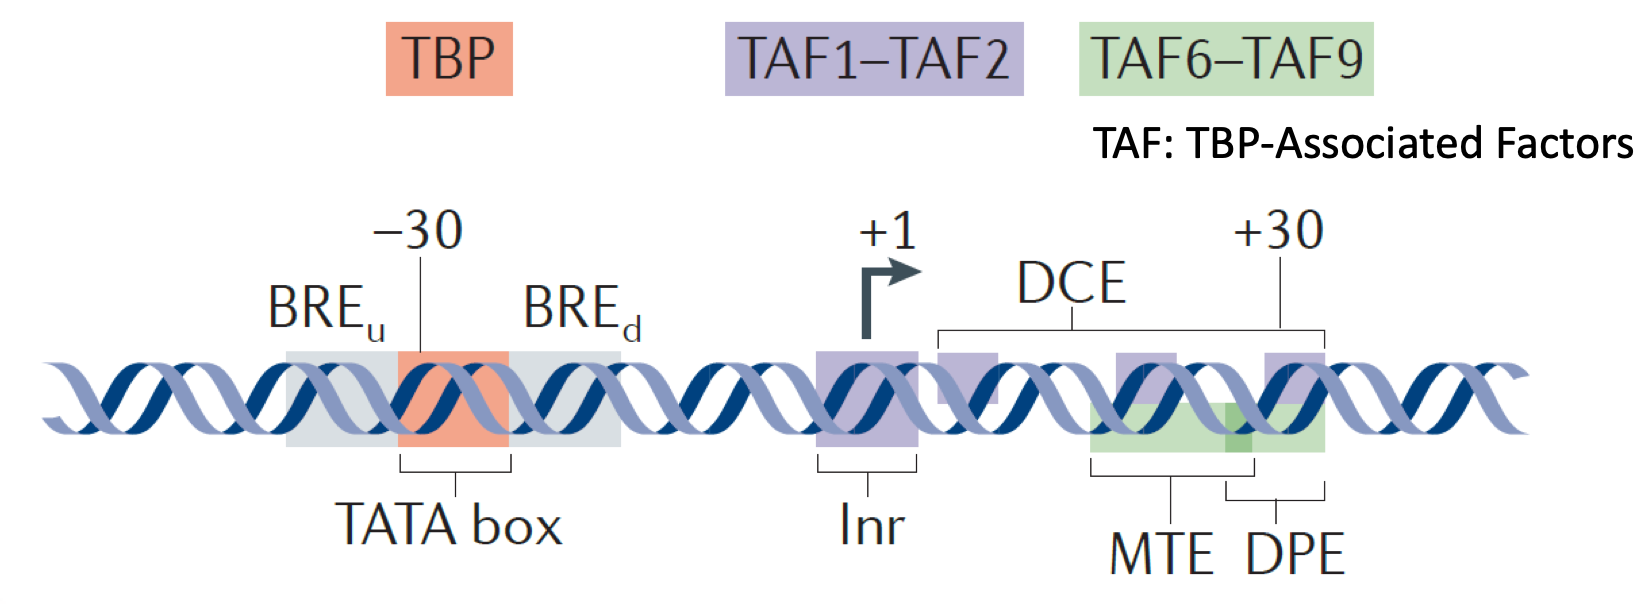
\includegraphics[width=0.5\textwidth]{../_resources/Screenshot_2022-09-16_at_12-11-22.png}
\caption{Sainsbury et al., Nature Review Mol. Cell. Biol. 2015}
\end{figure}

Once TFIIA and TFIIB reach TFIID, the upstream promoter complex forms. In particular, the promoter region becomes bent. Lastly, Pol II and TFIIF are recruited at the promoter region to initiate transcription.

\begin{figure}
\centering
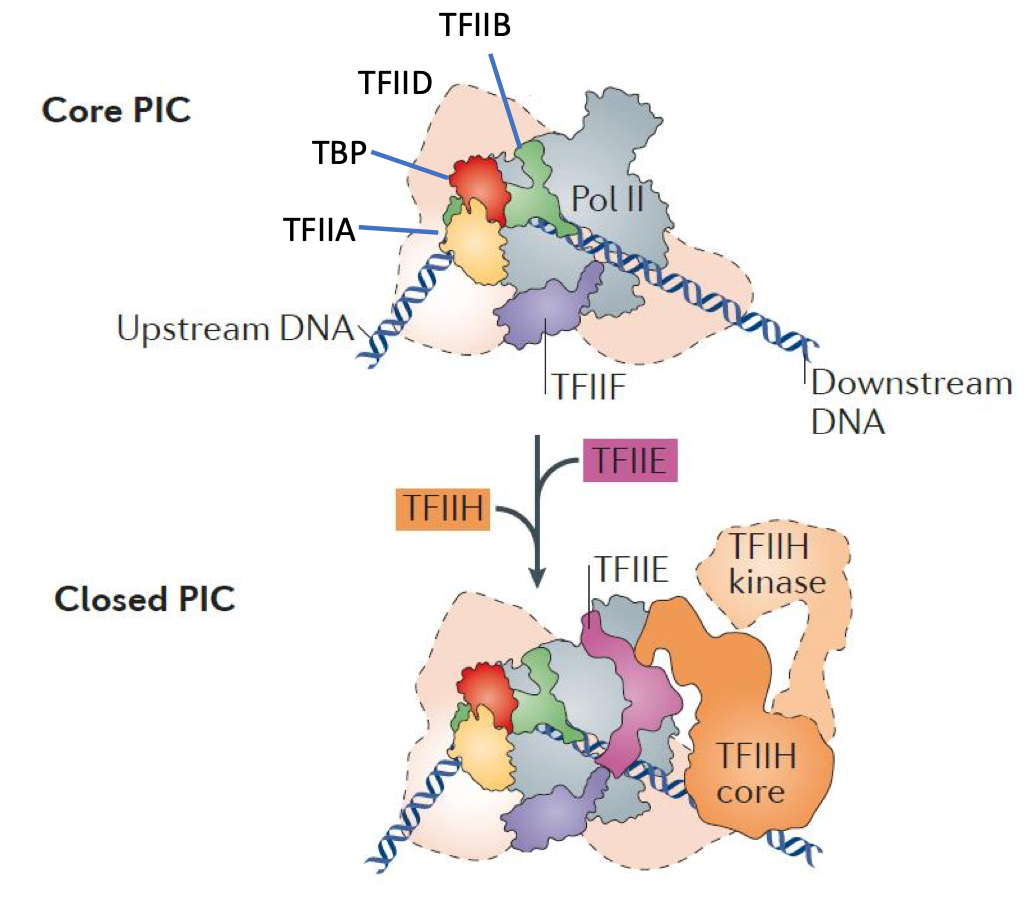
\includegraphics[width=0.5\textwidth]{../_resources/Screenshot_2022-09-16_at_15-53-19.png}
\caption{Sainsbury et al., Nature Review Mol. Cell. Biol. 2015}
\end{figure}

Once ATP is released, promoter clearance is activated allowing the PIC complex to reach the open conformation and to start transcription. \textbf{TFIIH} induces torsional stress by rotating with respect to a fixed site (TBP bound), melting DNA leading to the open complex state (OC). TFIIH promotes unwinding of approximately 10 bp of promoter DNA. When Pol II locates the TSS, it transits into a processive elongation mode. Dissociation of general transcription factors enables the formation of the Pol II elongation complex (addition of elongation factors).

Summarising, transcription initiation follows:

\begin{enumerate}
\def\labelenumi{\arabic{enumi}.}
\tightlist
\item
  TFIID + TBP promoter recognition $\rightarrow$ PIC assembly
\item
  TFIIA recruitment stabilises the TBP-DNA complex
\item
  TFIIB stabilises TBP-DNA and TBP-DNA-Pol II complexes, binds the template strand to position DNA for initiation of RNA syntehsis (setting the TSS); stimulates RNA synthesis by allosterically rearranging active site residues and stabilizing closed polymerase clamp
\item
  TFIIF heterodimer associates with polII and prevents non-specific interaction of polII with DNA; stabilizes the PIC by interacting also with TFIIB; influences TSS selection; stimulates phosphodiester bonds formation
\item
  TFIIE binds pol II (clamp) and facilitates the recruitment of TFIIH to the initiation complex; provides a bridge between polII and TFIIH; binds single stranded DNA; TFIIE stabilizes the open promoter; facilitates ATPase/kinase activities of TFIIH
\item
  TFIIH opens promoter DNA, phosphorilates RNA pol II CTD; promotes translocation of ssDNA into polII cleft
\item
  Factors binding modify the structural conformation of the preassembled complex TFIID-TBP-promoter structure becomes visible to TFIIB and A, the hole structure is visible to RNAPol II-TFIIF which is a compelx and so on\ldots{}
\item
  Pol II is positioned at the core promoter by the combination of TFIID, TFIIA and TFIIB through protein-protein interactions and protein-DNA interactions
\item
  TFIIH then melts 10-15 bp of DNA in order to position the single strand template in the polII cleft (open complex) to initiate RNA synthesis
\item
  The CTD of PolII will be phosphorilated by the TFIIH kinase subunit during the first 30 bp of transcription when PolII loses its contacts with GTFs before proceeding onto the elongation stage
\end{enumerate}

How does this start?~\emph{What makes a promoter all of a sudden accessible to TBP and so to TFIID?}~ The DNA sequence is always there, what makes it visible/accessible to the general transcription factors?

\hypertarget{chromatin-remodeling}{%
\section{Chromatin remodeling}\label{chromatin-remodeling}}

Nucleosomes are the functional units of protein. In nucleosomes the position of each major groove facing the histone octamer is designed as a \textbf{superhelix location} (SHL), numbered from 0 at the Dyad to ±7.

Proteins cannot easily associate with DNA sequences that touch the nucleosomal histone surface. Nucleosomal DNA is bent around the histone octamer~--~target sequences can be distorted or unrecognizable. GC-rich sequences with AA, TT or TA dinucleotides spaces by 10 bp bend more easily and display higher affinity for the histone octamer~``nucleosome positioning sequences''.

Nucleosome unwrapping is influenced by histone PTMs. In particular, certain combinations of PTMs display synergistic effects. For instance, covalent modifications of histone proteins can significantly alter the organization and function of chromatin. Examples:

\begin{itemize}
\tightlist
\item
  acetylated H3K56 enhances the unwrapping of the DNA at the entry/exit sites of the nucleosome.
\item
  acetylated H4K91 leads to nucleosome instability - H4K91 lays in the H3-H4 and H2A-H2B interaction surface
\end{itemize}

Histone modifications may also recruit proteins and enzyme to regulate the chromatin state. Remember that nucleosomal fibers can fold into higher order structures that may be even less accessible.

With the use of energy nucleosomes can be remodelled:
\begin{itemize}
\tightlist
\item
Histone octamers can slide along DNA
\item
Can be fully or partially disassembled
\item
Histones can be replaced with histone variants and post-translationally modified
\end{itemize}

These processes are carried out by the synergic activity of \textbf{chromatin remodeling complexes} and \textbf{histone chaperones}.

\hypertarget{techniques-to-study-chromatin-remodelling}{%
\subsubsection{Techniques to study chromatin remodelling}\label{techniques-to-study-chromatin-remodelling}}

\begin{itemize}
\tightlist
\item
  \textbf{MNase:} micrococcal nuclease is able to digest linker DNA, therefore to isolate nucleosomes. We have no information about the sequence, but we can assess the bp length of isolated DNA. Cons: some mapped entities are not nucleosomal, preference for cutting A/T rich regions.
\item
  \textbf{ChIP-seq}: after DNA sonication, immunoprecipitation and immunocomplex purification are performed (with protein-specific antibodies). DNA and proteins are cross-linked and purified, then bound DNA is analyzed by massively parallel short-read sequencing. ChIP-seq is relatively simple (technically), but does not have a high resolution due to non-uniform DNA fragmentation. Resolution also depends on library/sequencing setting.
\end{itemize}

\hypertarget{nucleosome-organization}{%
\section{Nucleosome organization}\label{nucleosome-organization}}

Nucleosome organization can be described as a combination of nucleosome occupancy and positioning:

\begin{itemize}
\tightlist
\item
  \emph{Occupancy}: average number of nucleosomes measured within a specific genomic region within a cell population
\item
  \emph{Positioning}: probability of a nucleosome reference point being at a specific genomic coordinate (same dyad)
\end{itemize}

Most nucleosomes in animal genomes are poorly positioned, but there are regions with \textbf{phased arrays} of well positioned nucleosomes (Figure \ref{fig:nucleosome}) .

\begin{figure}
\centering
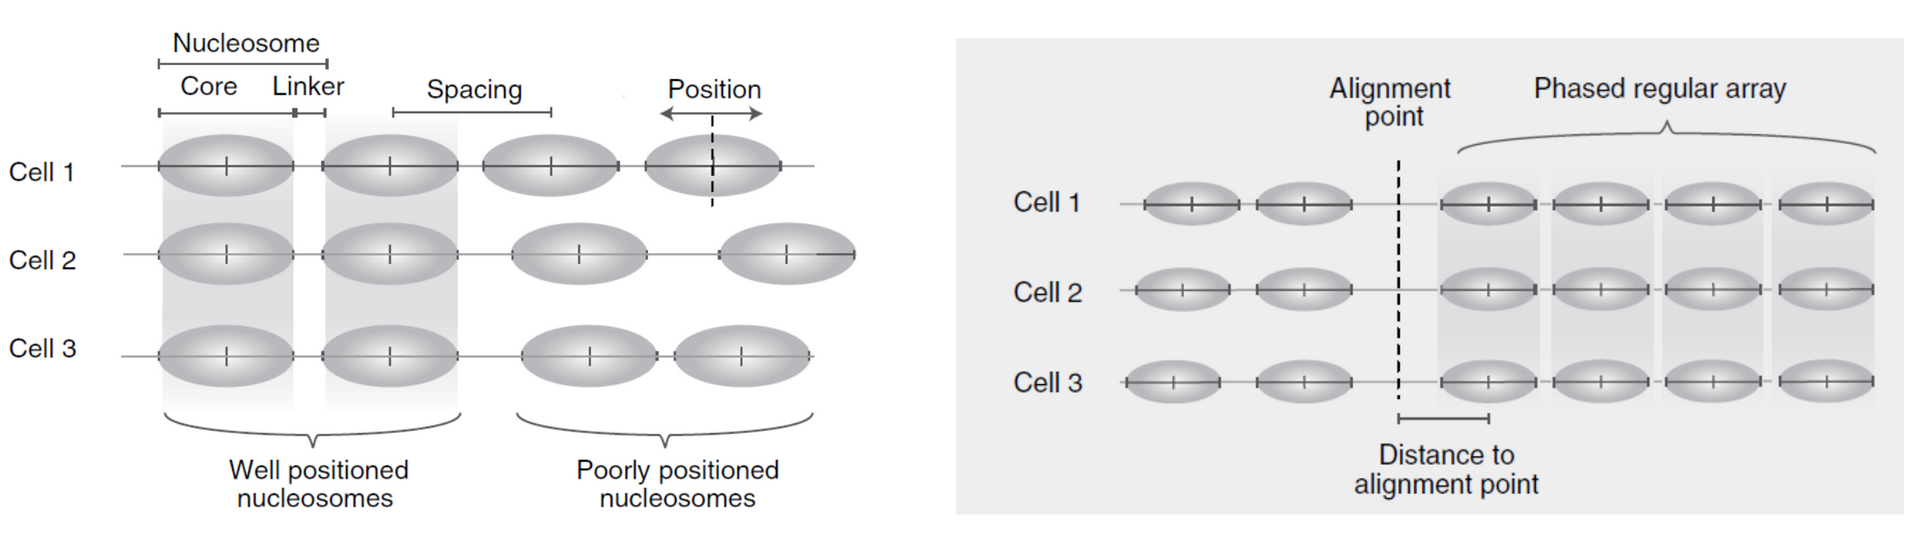
\includegraphics[width=0.7\textwidth]{../_resources/Screenshot_2022-09-16_at_16-26-04.png}
\caption{Nucleosome occupancy}
\label{fig:nucleosome}
\end{figure}

Most promoters contain a nucleosome free region (NFR) and a defined nucleosomal architecture that aids the recruitment of Pol II. A subset of genes may have a nucleosome in their promoter region, which is depleted during gene activation. DNA sequences containing relatively high GC content tend to wrap nucleosomes with higher affinity in vitro.

ATP-dependent chromatin remodellers act at promoter regions. \textbf{Remodels the structure of chromatin (RSC)} is a chromatin remodelling factor acting on core promoters. It retains a cavity which can accomodate nucleosomes.

\hypertarget{nucleosome-remodelling}{%
\subsection{Nucleosome remodelling}\label{nucleosome-remodelling}}

\begin{figure}
\centering
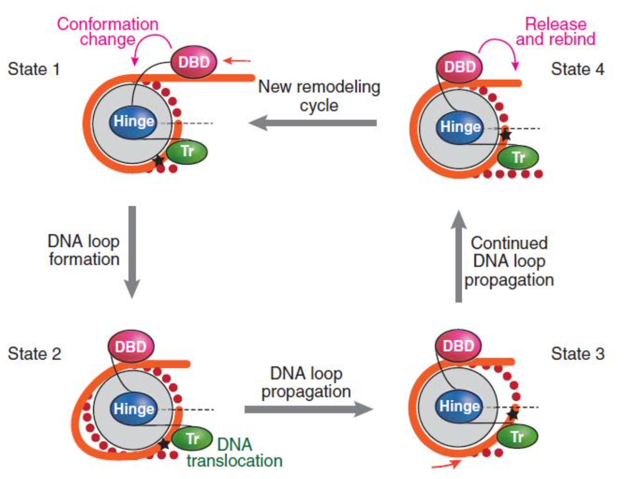
\includegraphics[width=0.5\textwidth]{../_resources/Screenshot_2022-09-16_at_16-30-29.png}
\caption{Becker and Workman, Cold Spring Harbor Laboratory, 2013}
\label{fig:peeling}
\end{figure}

The unpeeling of DNA segments from the histone surface can lead to a delocalization of nucleosomes (their sliding), removal or replacement of histones or to the complete eviction of the nucleosome, also dependent on associated histone chaperones (Figure \ref{fig:peeling}).

ATP-dependent chromatin remodelling enzymes can act cooperatively with \textbf{histone chaperones} to generate or disassemble nucleosomes. Chaperones associate with histones upon their synthesis, escort them into the nucleus, and aid in their specific association with DNA during different processes such as DNA replication, repair, or transcription. Histone Chaperones participate in assembly or disassembly nucleosomes in vitro or in vivo without using the energy of ATP.

Example: SWR and Inositol-requiring protein 80 (INO80) chromatin remodelling complexes regulate histone turnover and histone variant H2A.Z deposition. HIRA complex regulates H3.3 deposition at genes and regulatory elements.

\textbf{H2A.Z} has extended acidic patches on the surface which stimulate remodeling activities and weaken DNA interaction and may play a role in Pol II recruitment - it is lost at promoters upon RNA PolII loading. H2A.Z comprises 15\% of total H2A and it is post translationally modified (acetyated, polyubiquitinilate\ldots).

The most rapid \textbf{nucleosome turnover} occurs over promoters, tRNA, and small nucleolar RNA genes (often studied in over expression settings).

\begin{figure}
\centering
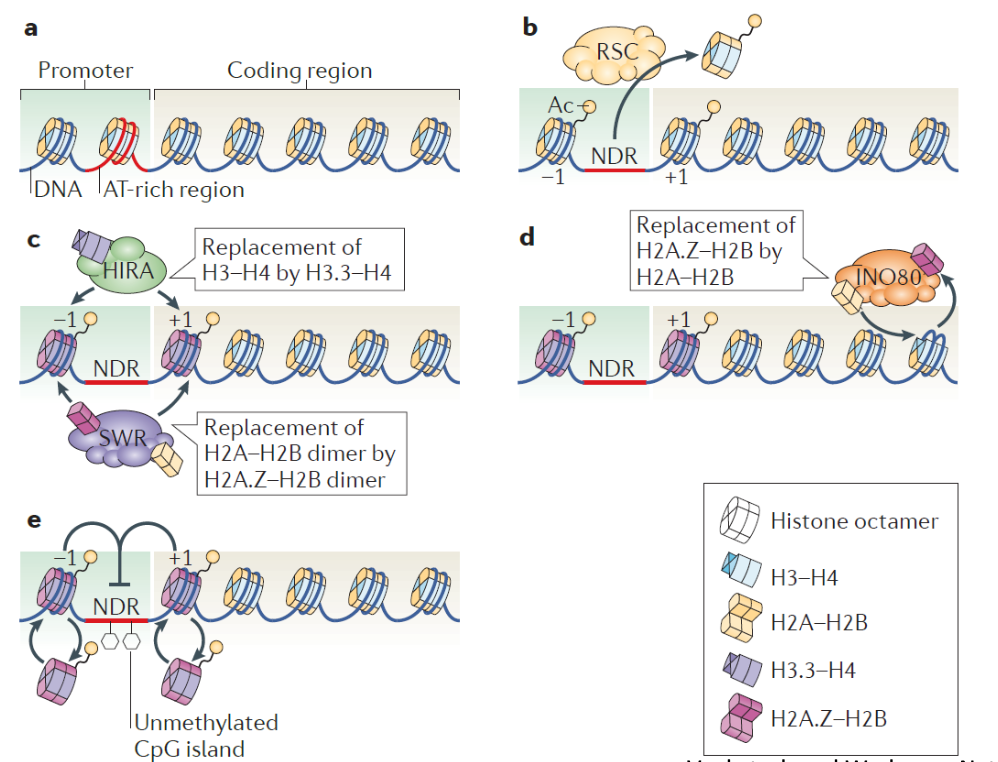
\includegraphics[width=0.5\textwidth]{../_resources/Screenshot_2022-09-23_at_15-22-44.png}
\caption{Venkatesh and Workman, Nature Rev Mol Cell Biol, 2015}
\label{fig:pronucleo}
\end{figure}

PIC formation at a core promoter requires a nucleosome depleted region (Figure \ref{fig:pronucleo}). This could be achieved by \textbf{RSC} binding to the AT-rich region in the promoter, freeing the NDR. Next, \textbf{HIRA} performs the replacement of H3-H4 by H3.3-H4 and \textbf{SWR} replaces the H2A-H2B dimer by H2A.Z-H2B dimer. Finally, \textbf{INO80} replaces H2A.Z-H2B by H2-A and H2B. The resulting scenario exhibits unmethylated CpG islands in NDR region, allowing for PIC formation.

\subsection{Chromatin Immunoprecipitation} 
(ChIP) experiments to determine protein-DNA interactions require a \emph{crosslinking} step.

\begin{enumerate}
\tightlist
\item
  Crosslinking: formaldehyde and a quencher are required to covalently modify DNA

\begin{figure}
\centering
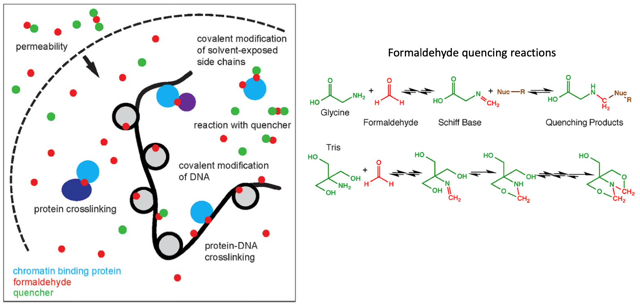
\includegraphics[width=0.5\textwidth]{../_resources/Screenshot_2022-09-22_at_21-36-39.png}
\caption{Cross linking}
\end{figure}

\item
  Lysis
\item
  Antibody binding
\item
  Immunoprecipitation
\item
  Wash steps
\item
  Crosslink reversal
\item
  DNA purification and quantitative PCR
\item
  DNA and protein analysis
\end{enumerate}
 Chromatin Immunoprecipitation coupled to sequencing analyses can be used to determine protein-DNA interactions.
 
\hypertarget{main-nucleosome-modifications-in-promoters}{%
\subsection{Main nucleosome modifications in promoters}\label{main-nucleosome-modifications-in-promoters}}

Most promoters (98\%) occupied by Pol II are also occupied by histone H3K4me3 and acetylated H3K9 and H3K14 (Gunter et al., 2007).

\begin{itemize}
\tightlist
\item
  \textbf{H3K4me3}-modified nucleosomes are found at sites of transcription. H3K4me3 enrichment is detectable in almost 80\% of all protein-coding genes within 1 kb of known or predicted transcript start sites. Only 30-40\% of protein coding genes are expressed in human embryonic stem cells. Histone H3K4me3 is observed also at the promoters of genes for which there is no evidence of transcription in ES cells - typically lower than in active genes. Genes not enriched in H3K4me3 are found in clusters along the genome; The vicinity of these genes on the genome suggest that their expression they may be regulated sinergically.
\item
  \textbf{H3K9-14Ac} were enriched at the promoters of nearly 70\% of genes, including both transcriptionally active and inactive genes. Nearly all of the promoters (\textgreater95\%) acetylated on H3K9 and H3K14 were also enriched for H3K4me3.
\item
  \textbf{H3K36me3} and \textbf{H3K79me2} modifications occur almost exclusively downstream of promoters that produce detectable transcripts in ES cells
\end{itemize}

\hypertarget{rt-qpcr-based-detection-of-5-rna-transcripts-of-inactive-genes}{%
\subsubsection{RT-qPCR based detection of 5' RNA transcripts of inactive genes}\label{rt-qpcr-based-detection-of-5-rna-transcripts-of-inactive-genes}}

\begin{enumerate}
\def\labelenumi{\arabic{enumi}.}
\tightlist
\item
  Assay components and DNA template: forward primer + probe + reverse primer
\item
  Denatured template and annealing assay components:
\item
  Polymerization and signal generation
\end{enumerate}

Genes that do not produce full length mRNAs can experience transcription initiation. The majority of all genes contain H3K4me3-modified nucleosomes in both ES and differentiated cells. Differential H3K4 methylation is found in 25\% of genes. These genes have cell type-specific expression pattern and cell type-specific function.

\begin{figure}
\centering
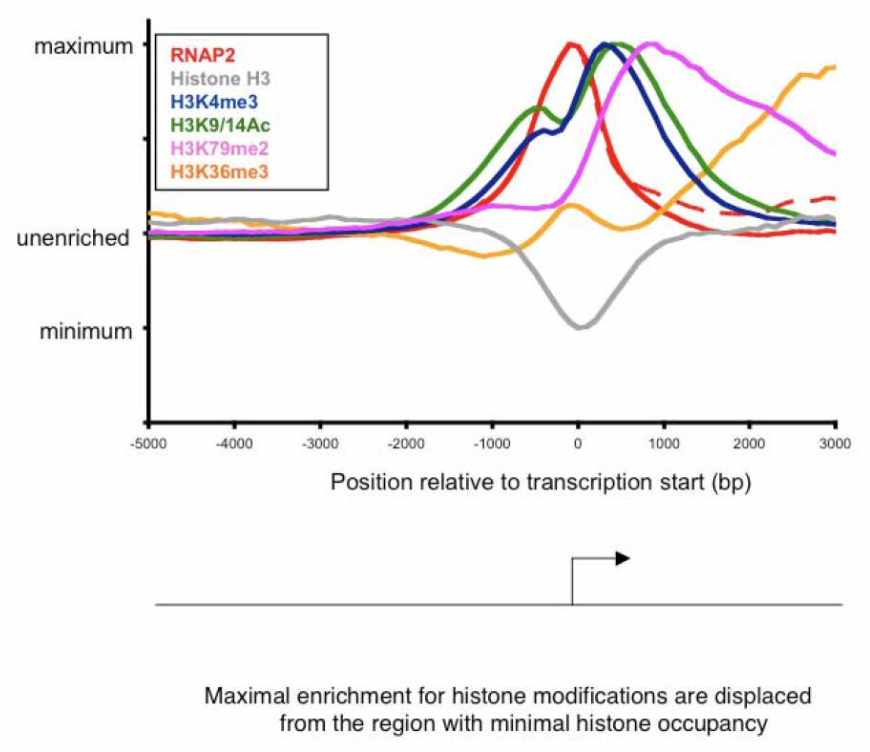
\includegraphics[width=0.5\textwidth]{../_resources/Screenshot_2022-09-22_at_21-49-05.png}
\caption{Guenther et al., Cell 2007}
\end{figure}

\textbf{Summary:} Results suggest that most protein-coding genes in human cells, including most genes thought to be transcriptionally inactive, experience the hallmarks of transcription initiation. H3K4me3 and H3K9-14Ac modifications, together with RNA Pol II, occupy the promoters of approximately 79\% of protein-coding genes in ES and differentiated cells, but only about half of these produce detectable transcripts. The co-occupancy of Pol II with H3K4me3- and H3K9,14Ac-modified nucleosomes at genes without detectable levels of transcription suggests that a large fraction of human genes experience transcription initiation without transcript completion.

Protein-coding genes can fall into three groups of regulatory behaviour:

\begin{itemize}
\tightlist
\item
  \emph{Productive}: the actively transcribed genes are occupied by nucleosomes with histone modifications that are hallmarks of both initiation (H3K4me3 and H3K9-14Ac) and elongation (H3K36me3 and H3K79me2)
\item
  \emph{Non-productive}: experiences transcription initiation without evidence of transcript elongation or accumulation.
\item
  \emph{No initiation}: genes that are excluded from experiencing transcription initiation, where mechanisms that prevent transcription initiation must predominate.
\end{itemize}

\hypertarget{global-run-on-sequencing-gro-seq}{%
\subsubsection{Global run-on sequencing (GRO-seq)}\label{global-run-on-sequencing-gro-seq}}

Global run-on sequencing (GRO-Seq) enables to map the presence of elongating RNA pol in the chromatin context by detection of the nascent transcripts. The \emph{Sarkosyl treatment} permeabilizes nuclear membranes, prevents RNA Pol from binding DNA (if not already bound), disassembles chromatin and dissociates pausing factors.

\begin{figure}
\centering
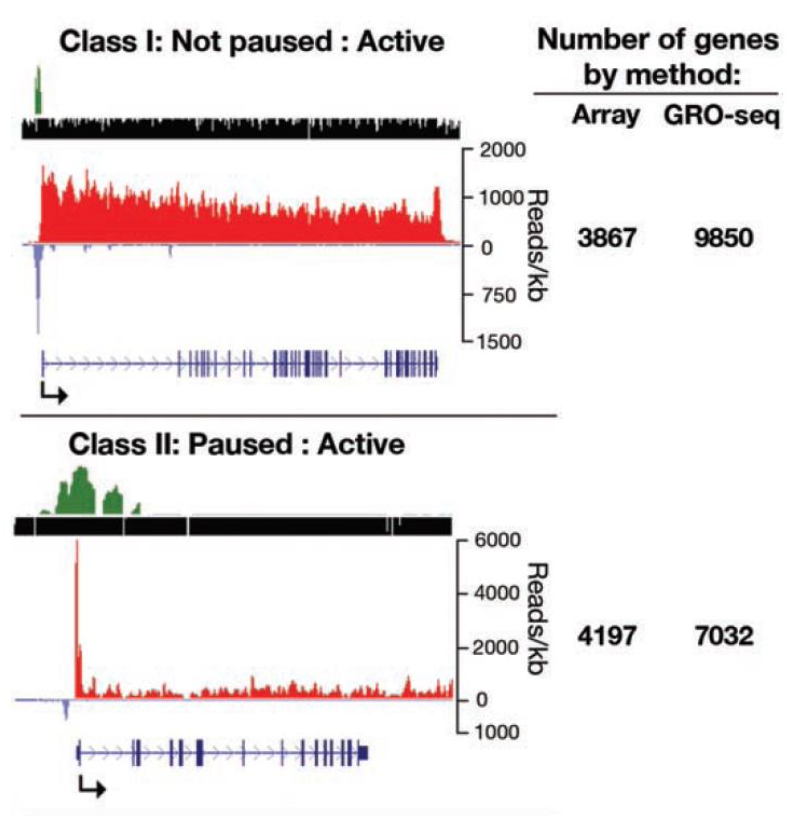
\includegraphics[width=0.5\textwidth]{../_resources/Screenshot_2022-09-22_at_21-58-03.png}
\caption{Core et al, 2008}
\end{figure}

Results: only few paused genes are transcriptionally inactive.
\textbf{Pausing} can be seen as a mechanism for tuning expression from active genes rather than a means of gene inactivation. The paused Pol II remains stably associated with the nascent RNA and is fully capable of resuming elongation; however, further signals are needed to elicit the transition to a productive elongation complex.

\emph{Pausing index}: ratio of Pol II density on promoter to gene body.

The \textbf{CTD} undergoes dynamic changes in phosphorylation and dephosphorylation during transcription. The CTD is a long unstructured domain consisting of \(Y_1S_2P_3T_4S_5P_6S_7\) tandem repeats. \textbf{Cyclin-dependent kinases} (CDKs) are serine/threonine specific kinases; cell cycle-associated CDKs regulate cell cycle progression. Transcription-associated CDKs are key regulators of gene expression. PTMs of the PolII CTD coordinate transcription and RNA processing

\begin{figure}
\centering
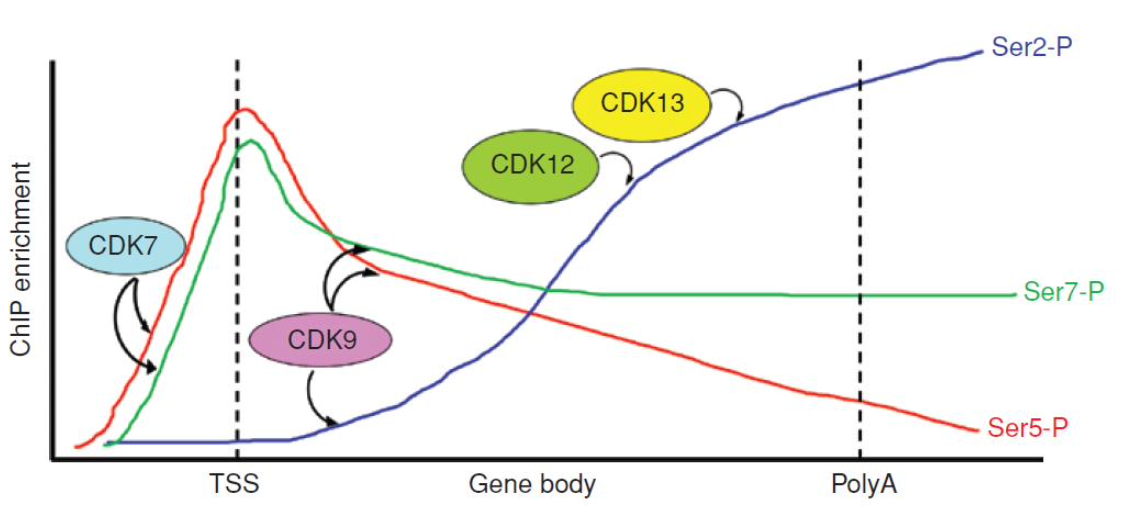
\includegraphics[width=0.5\textwidth]{../_resources/Screenshot_2022-09-22_at_22-09-19.png}
\caption{Differential phosphorylation of RNA Pol II CTD during transcription.}
\label{fig:phCTD}
\end{figure}

The differential phosphorylation of RNA Pol II CTD during transcription is reported in Figure \ref{fig:phCTD}.

\hypertarget{transcription-pausing-mechanism}{%
\subsubsection{Transcription pausing mechanism}\label{transcription-pausing-mechanism}}

\textbf{NELF} is recruited on PolII by \textbf{DSIF}, which contributes to pausing by forming 2 nucleic acid clamps. CDK9 with cyclin T, referred to as \textbf{P-TEFb} complex, enables pause-release leading to transcription elongation (Figure \ref{fig:dsif}) .

\begin{figure}
\centering
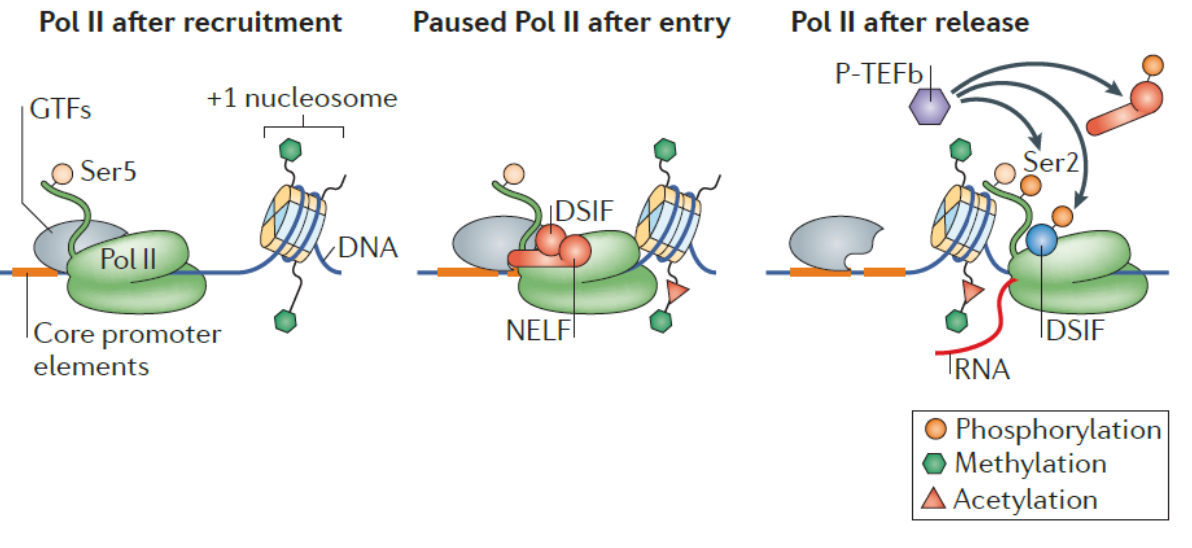
\includegraphics[width=0.5\textwidth]{../_resources/Screenshot_2022-09-22_at_22-14-15.png}
\caption{Jonkers \& Lis, Nature Rev Mol Cell Biol, 2015}
\label{fig:dsif}
\end{figure}

Pol II distribution profiles surrounding all promoters reveal a general decrease in promoter occupancy upon NELF depletion. Knockdown of NELF and consequent reduced Pol II pausing decreases gene expression, because nucleosomes occupy the promoter regions and thus block the expression of these genes by preventing TF and GTF binding.

\textbf{Promoter-proximal pausing} represents an additional layer of regulation to accommodate increased demands for precise and rapid gene regulation during organism development and responses to stress. It might be beneficial to maintain highly regulated promoters poised in an open chromatin state, to prevent their incorporation into the more inaccessible, condensed heterochromatin that exists in metazoans. Housekeeping genes lack pronounced pol II pausing.

Main hypotheses for the function of pol II pausing:

\begin{itemize}
\tightlist
\item
  establishing permissive chromatin: paused Pol II helps to maintain the nucleosome-deprived structure by blocking nucleosome assembly over promoter sequences. Pausing would thus keep the promoter region accessible for activator and transcription factor binding.
\item
  rapid or synchronous activation: at a gene with paused Pol II, gene activation could proceed simply through recruitment of positive transcription elongation factor b (P-TEFb), thereby triggering the rapid release of paused Pol II into productive elongation without the need of the PIC assembly.
\item
  integration of signals: pausing represents a separate step in the transcription cycle for factors to act and allows for combinatorial control between transcription factors that recruit the transcription machinery (TF1) and those that trigger pause release (TF2), where both would be necessary for gene activation.
\item
  checkpoint in early elongation: on the left, arrows depict interactions between the capping enzyme complex (CEC) and DSIF--NELF as well as the Ser5 phosphorylation of the carboxy-terminal heptapeptide repeat domain (CTD) of Pol II, which is thought to stimulate capping activity. The hat represents the 5 RNA cap. In the centre, P-TEFb-dependent phosphorylation events release paused Pol II and create a platform for binding of RNA-processing factors (RPFs) on the Ser2-phosphorylated CTD of Pol II, as shown on the right.
\end{itemize}

7SK snRNP represses transcription by sequestering and inhibiting P-TEFb. Super elongation complex (\textbf{SEC}) and Bromodomain containing protein 4 (\textbf{BRD4}) complexes represent active forms of P-TEFb that can promote the release of Pol II from pausing.

\textbf{BRD4} competes for binding to P-TEFb with the P-TEFb inhibitory complex HEXIM-- 7SK, and it is recruited to TSSs by multiple means, including histone acetylation. The SEC can interact with a subset of co-activators such as Mediator, polymerase- associated factor 1 (PAF1) and Integrator, the latter of which is a complex that interacts with the CTD of Pol II. The SEC and BRD4 predominantly mediate the recruitment P-TEFb, but their regulatory importance and composition with regard to paused Pol II release seems to vary across different genes, cell types and stimuli. Ser2 phosphorylated CTD promotes the recruitment of other transcription elongation factors, including SPT6.

A large repertoire of transcription activators crucially involved in cancer, including MYC and NF-kB, target P-TEFb, DSIF or NELF to gene promoters.

\section{Transcription elongation}

During the elongation phase, RNA pol II faces nucleosomes. In order to proceed with elongation, RNA pol II needs to overcome the issue: \emph{histone turnover} is predominantly observed at transcription start sites.

\hypertarget{structural-basis-of-the-nucleosome-transition-during-rna-pol-ii-passage---kujirai-et-al-2018}{%
\subsection{Structural basis of the nucleosome transition during RNA pol II passage}\label{structural-basis-of-the-nucleosome-transition-during-rna-pol-ii-passage---kujirai-et-al-2018}}

The aim of the research paper was to reconstitute RNA pol II and a nucleosome separately in vitro and analyze their interaction. The DNA stretch is required to be around 153 bp to achieve histone wrapping for obtaining a nucleosome. Keep in mind that is not easy to recapitulate the PIC formation in vitro. The fist step involves unwinding and exposing DNA. For bypassing this step, it is possible to use an already ``melted'' initiation site ready for transcription. Once RNA pol II and \textbf{TFIIS} elongation factor are added, transcription can start.

\hypertarget{nucleosome-structure}{%
\subsubsection{Nucleosome structure}\label{nucleosome-structure}}

A single base pair is centred on the nucleosome \emph{dyad}, which defines the pseudo 2-fold symmetry axis of the nucleosome. The major groups in the DNA stretch facing the dyad are \emph{superhelical location} (SHL) -7 and -1. In nucleosomes, SHLs are formed at regular intervals (10bp) from the dyad interacting with histone K and R residues.

\begin{figure}
\centering
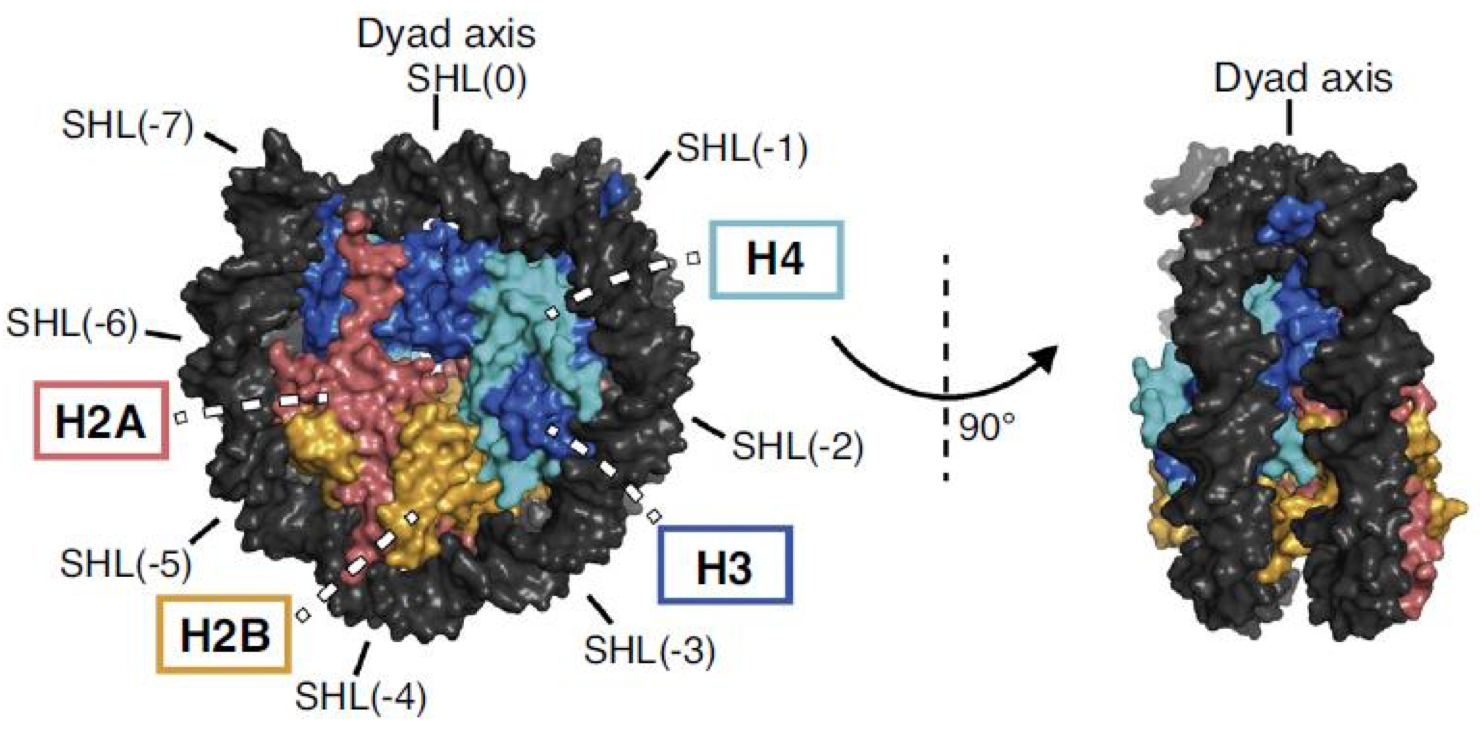
\includegraphics[width=0.5\textwidth]{../_resources/Screenshot_2022-10-05_at_22-41-07.png}
\caption{Kujirai and Kurumizaka, \emph{Curr Op. Struct. Biol.,} 2020}
\end{figure}

Kujirai and Kurumizaka, \emph{Curr Op. Struct. Biol.,} 2020

\hypertarget{cryo-em}{%
\subsubsection{Cryo-EM}\label{cryo-em}}

Cryo-Electron Microscopy is technique applied for molecule structure determination, which allows to reconstruct structures almost at the atomic level. We freeze samples in vitro (-80° C, -90° C) with liquid ethane. The sample is hit with a photon beam instead of light from different orientations, obtaining a pool of 2D images. Finally, a 3D image is reconstructed through an algorithm, providing a resolution in Armstrongs.

\begin{figure}
\centering
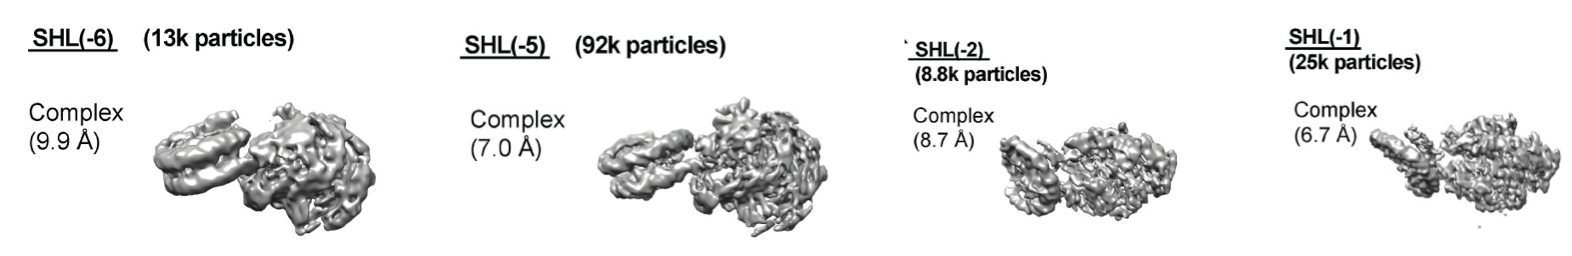
\includegraphics[width=0.5\textwidth]{../_resources/Screenshot_2022-10-05_at_22-57-06.png}
\caption{Screenshot 2022-10-05 at 22.57.06.png}
\end{figure}

Most of the times, RNA Pol II was associated with the nucleosome at position SHL(-5) or SHL(-1), as well as SHL(-6) and SHL(-2). Other sites were quickly encountered and passed by Pol II, whereas the aforementioned ones required a bit more time. Looking at the electrophoresis results without the addition of TFIIS, RNA pol II can only reach SHL(-5), while when we add it also SHL(-1) is observed.

RNA Pol II elongates RNA up to SHL(-5) in the absence of the elongation factor and until reaching SHL(-1) in the presence of TFIIS. Pausing at SHL (-5) and (-1) represent rate limiting steps of nucleosomal transcription in vitro.

\begin{figure}
\centering
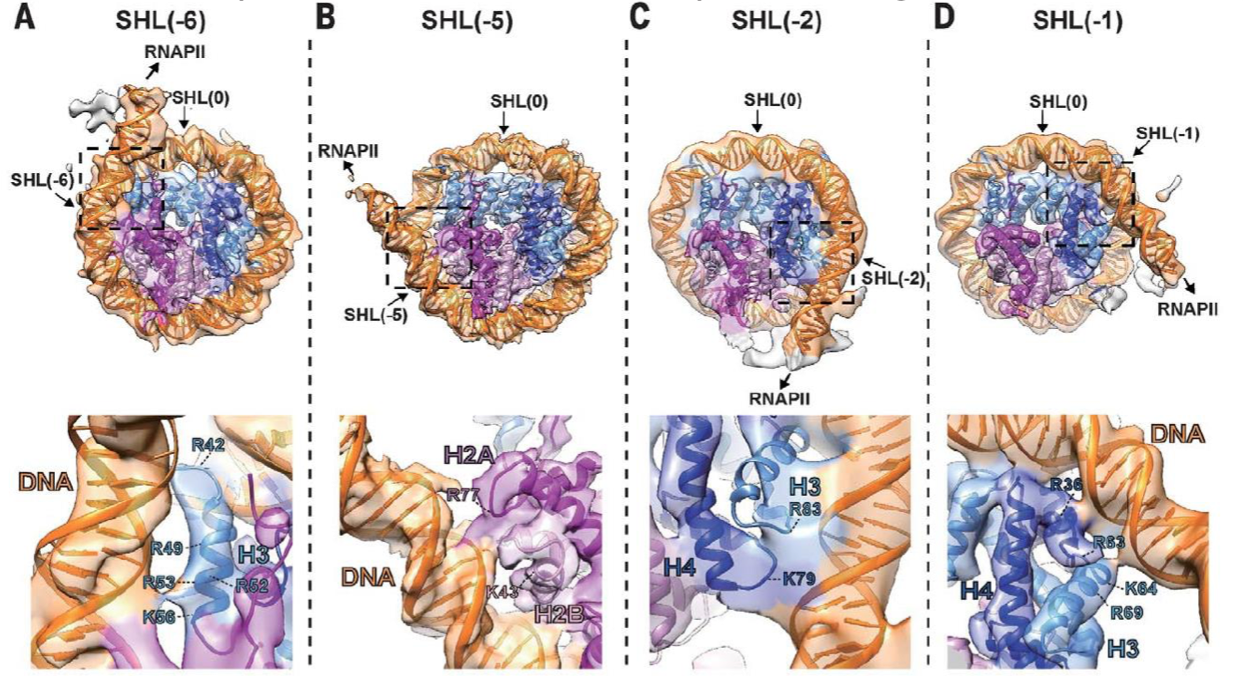
\includegraphics[width=0.5\textwidth]{../_resources/Screenshot_2022-10-05_at_22-54-39.png}
\caption{Kujirai at al., \emph{Science,} 2018}
\end{figure}

Kujirai at al., \emph{Science,} 2018

SHL(-6) is at the entry site, DNA has not been ``peeled'' yet from the nucleosome. At these sites H3 and H4 interact with DNA, we can appreciate the presence of modifications.

The dimer H2A and H2B is completely exposed after the ``peeling'' of the first DNA turn. This results in the uncovering of a positively charged region, which can be easily accessed by other compounds and rewrapped by ``foreign DNA'' i.e.~not the DNA which was there previously.

\begin{figure}
\centering
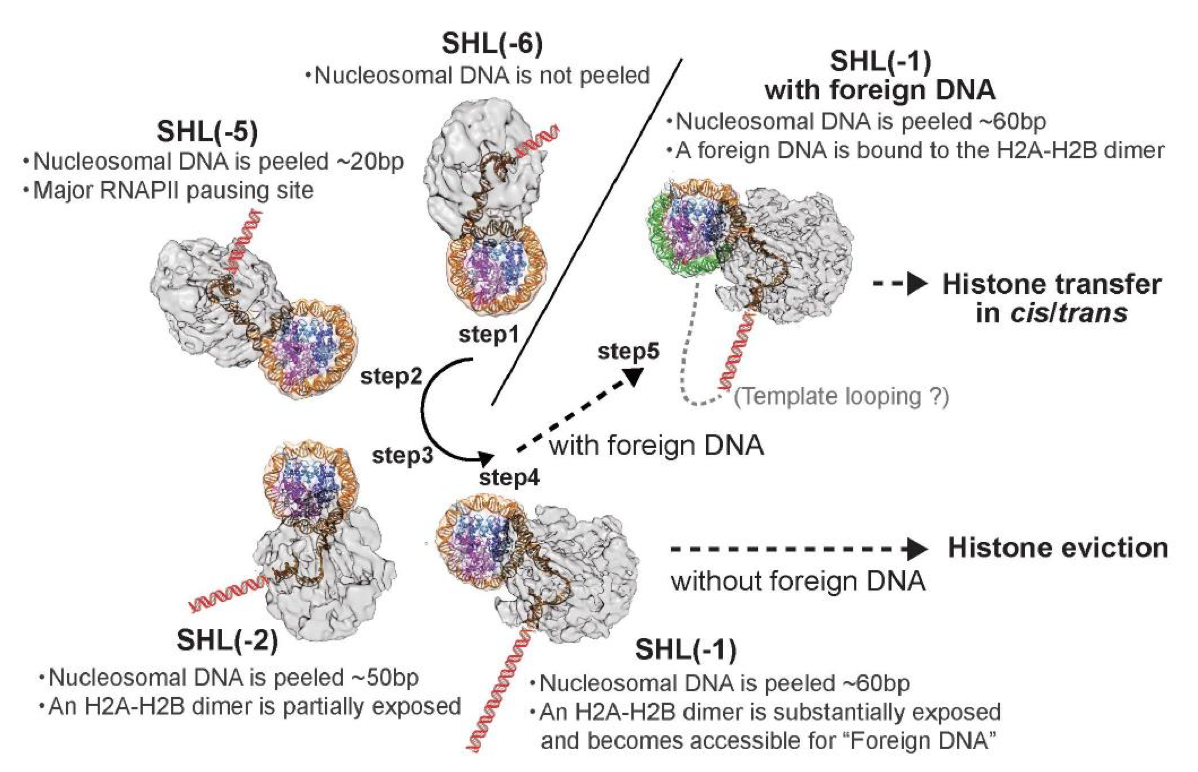
\includegraphics[width=0.5\textwidth]{../_resources/Screenshot_2022-10-05_at_23-02-04.png}
\caption{Screenshot 2022-10-05 at 23.02.04.png}
\end{figure}

\hypertarget{summary-of-the-main-results}{%
\subsubsection{Summary of the main results}\label{summary-of-the-main-results}}

\begin{itemize}
\tightlist
\item
  Nucleosomes can inhibit initiation and elongation of transcription.
\item
  Nucleosome free regions are present within core promoters.
\item
  Transcription pausing occurs at the first well-positioned nucleosome (+1).
\item
  RNA polII transiently pauses when it transcribes nucleosomal DNA.
\item
  Elongation factors are required for productive transcription.
\item
  The transcription efficiency is modulated by histone post-translational modifications, histone variants and histone exchange which may affect histone-DNA contacts in the nucleosome releaving the major RNAPII pausing sites.
\end{itemize}

\hypertarget{template-looping}{%
\subsubsection{Template looping}\label{template-looping}}

DNA upstream of Pol II starts wrapping around the upstream nucleosome, pushing pol II to continue. This process does not require disassembly.

\begin{figure}
\centering
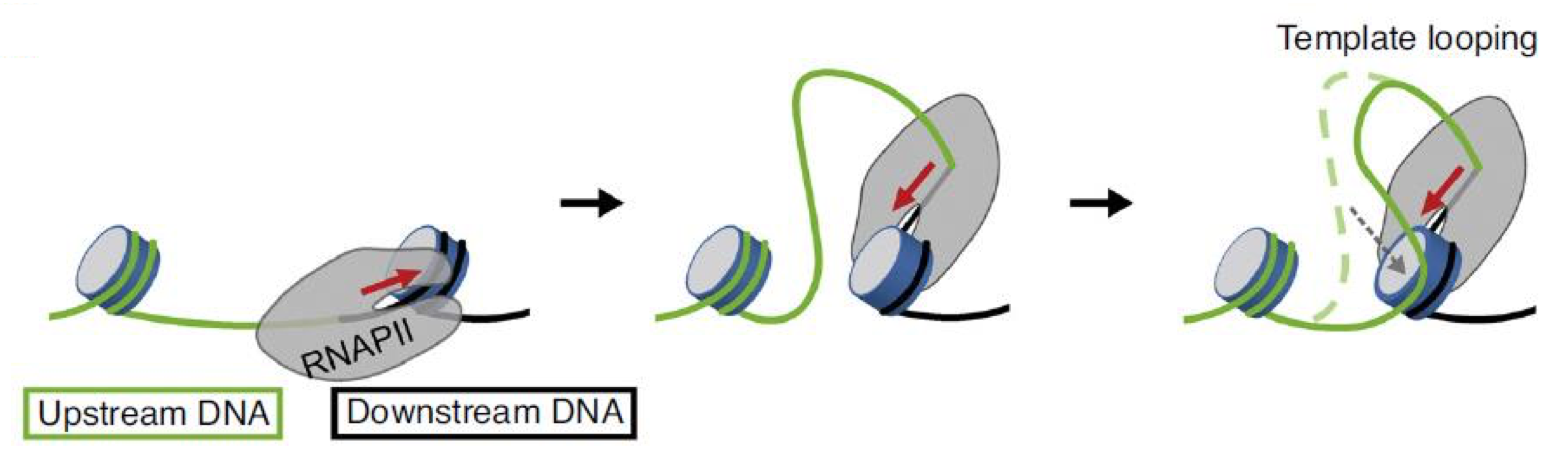
\includegraphics[width=0.5\textwidth]{../_resources/Screenshot_2022-10-05_at_23-04-42.png}
\caption{Kujirai and Kurumizaka., \emph{Curr Op. Struct. Biol.,} 2020
Template looping results in histone transfer from ahead of the transcribing RNApol II to behind}
\end{figure}

Kujirai and Kurumizaka., \emph{Curr Op. Struct. Biol.,} 2020
Template looping results in histone transfer from ahead of the transcribing RNApol II to behind

It is not only required to have TFIIS, other factors are involved: Spt4/5 and Paf1C (elongation factors), \textbf{FACT} and \textbf{Spt6} (histone chaperones) with acidic patches balancing the positively charged histones exposed in unwrapping.

\textbf{FACT}(facilitate chromatin transcription) interacts with the H2A-H2B dimer and we observe the formation of the \emph{hexasome} (only 8 subunits) in the process of histone turnover. FACT activity is also influenced by H2A-H2B dimers ubiquitylation. Nap1 (HC) stabilizes hexasomes favouring transcription elongation.

\begin{figure}
\centering
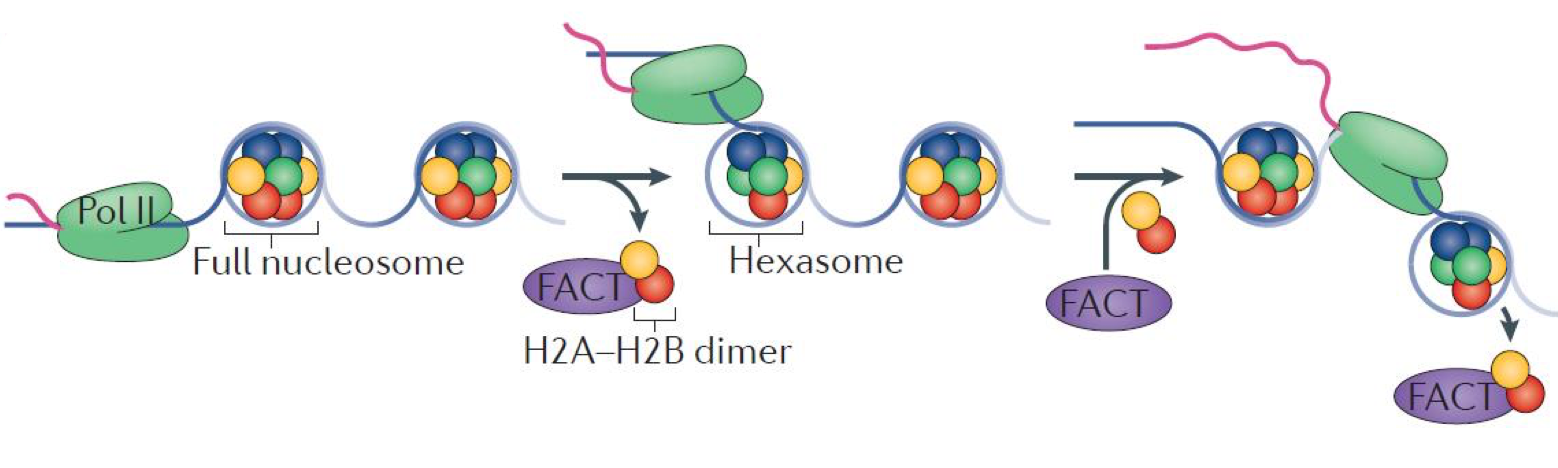
\includegraphics[width=0.5\textwidth]{../_resources/Screenshot_2022-10-05_at_23-05-01.png}
\caption{Lai and Pugh, \emph{Nature Review Mol Cell Biol}. 2017}
\end{figure}

Lai and Pugh, \emph{Nature Review Mol Cell Biol}. 2017

In a similar fashion, H3.3 is bound by HIRA, TF for ``recycling'', regulated by acetylation.

\textbf{Paf1C} elongation factor interacts directly with Pol II, in particular with s5 phosphorylation. It also interacts with DSIF and FACT. When pol II is elongating, it promotes the phosphorylation of NELF and DSIF. Ctr9 is a subunit of Paf.

\begin{figure}
\centering
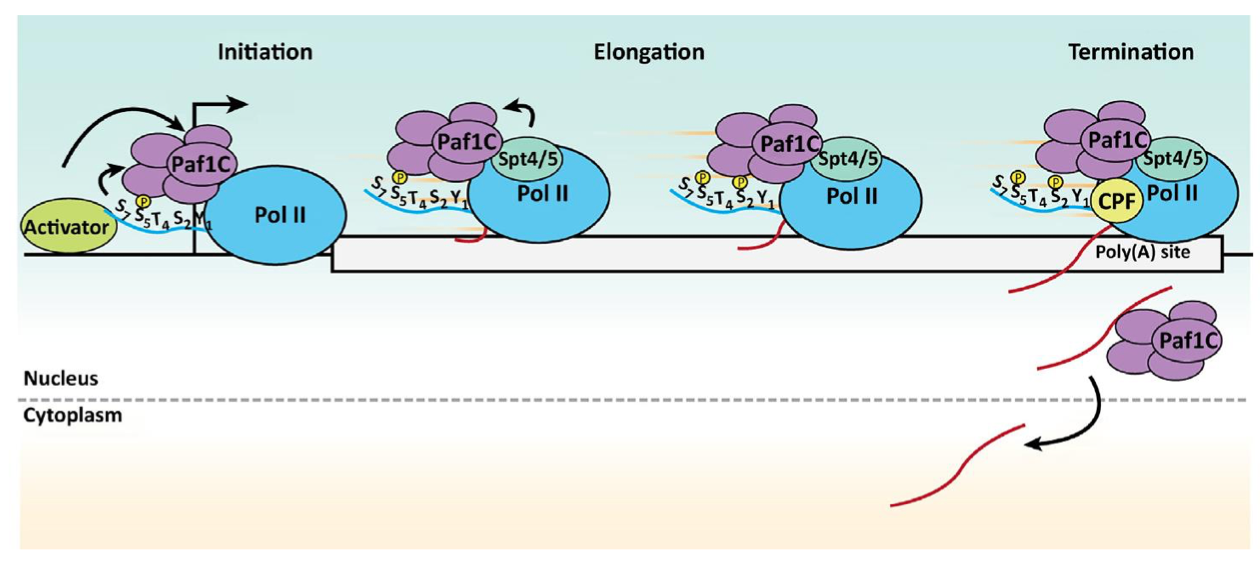
\includegraphics[width=0.5\textwidth]{../_resources/Screenshot_2022-10-05_at_23-05-58.png}
\caption{Van Oss \emph{et al., TRENDS Biochem Sci.} 2017}
\end{figure}

Van Oss \emph{et al., TRENDS Biochem Sci.} 2017

\hypertarget{structural-basis-of-nucleosome-disassembly-and-reassembly-by-rna-p-ii-elongation-complex-with-fact---ehara-et-al.}{%
\subsubsection{Structural basis of nucleosome disassembly and reassembly by RNA P II elongation complex with FACT - Ehara et al.}\label{structural-basis-of-nucleosome-disassembly-and-reassembly-by-rna-p-ii-elongation-complex-with-fact---ehara-et-al.}}

Recent article: once H2A-H2B are partially exposed, FACT starts interacting with the nucleosome. When the full exposure of the nucleosome is reached, FACT promotes a transit from downstream to upstream, assisting the template looping procedure.

\begin{figure}
\centering
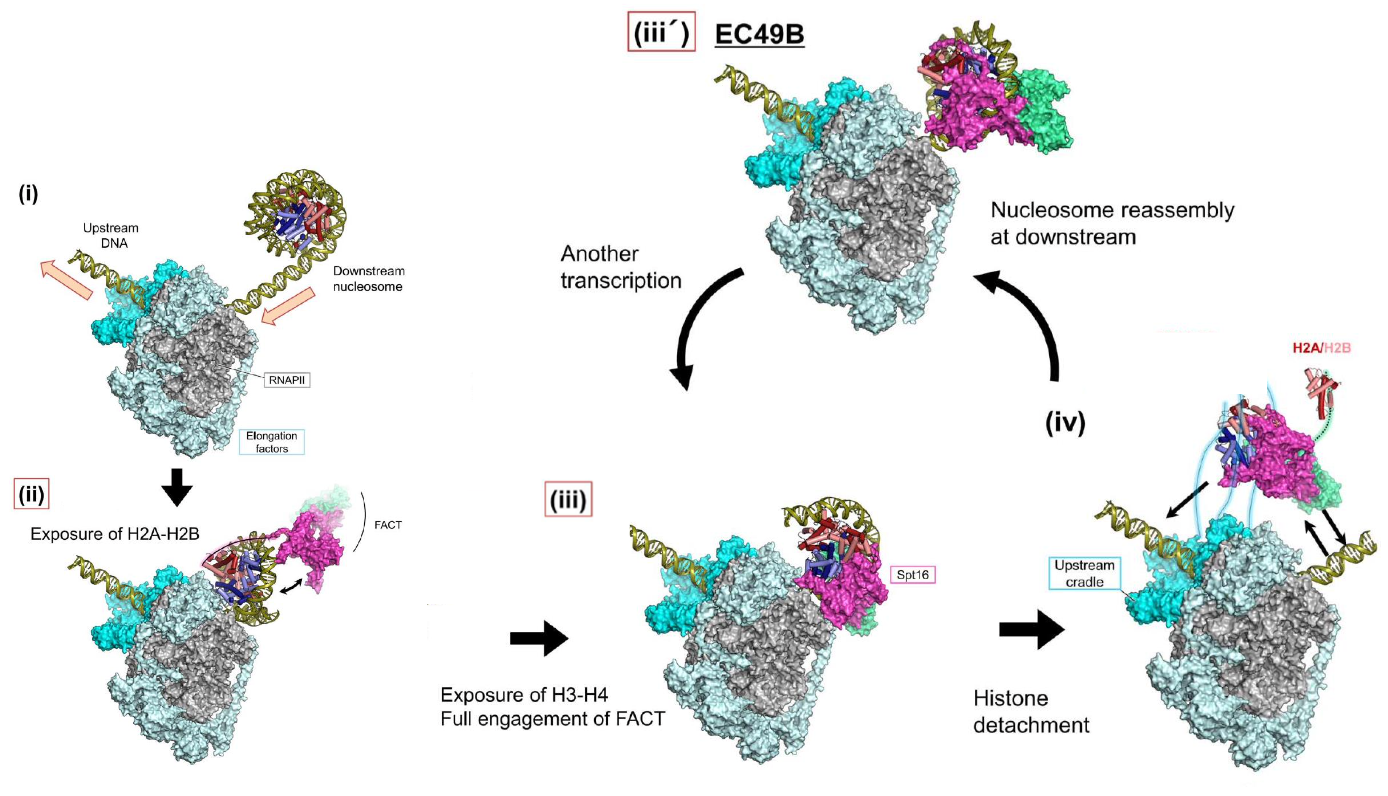
\includegraphics[width=0.5\textwidth]{../_resources/Screenshot_2022-10-10_at_10-35-12.png}
\caption{Screenshot 2022-10-10 at 10.35.12.png}
\end{figure}

Chromatin remodeling factors also partecipate in transcription elongation:

\begin{itemize}
\tightlist
\item
  \textbf{RSC}: arrangement of NDR between +1 and -1 nucleosomes
\item
  \textbf{CHD1} and \textbf{ISWI}: arrangement of nucleosome spacing and separation of closely packed nucleosomes
\item
  \textbf{Fun30}: facilitation of nucleosome disassembly
\end{itemize}

\hypertarget{termination}{%
\section{Transcription termination}\label{termination}}

Transcription termination occurs when the elongation complex is disassembled, and both RNA Pol II and the RNA are released. In our cells a signal on DNA is required, a \emph{polyA site} followed by U rich/G rich regions. Once polyA is transcribed, we observe the SPSF complex recruitment, which recognizes the AAA site and proceeds to RNA cleavage and polyadenylation. Meanwhile, RNA pol II will continue transcription (slowly, probably due to allosteric changes in pol II structure bound to the complex) of mRNA which will be degraded due to the exposed 5' end. \textbf{\emph{Torpedo model:}} XRN2 degrades this RNA and leads to the dissociation of pol II from DNA.

\begin{figure}
\centering
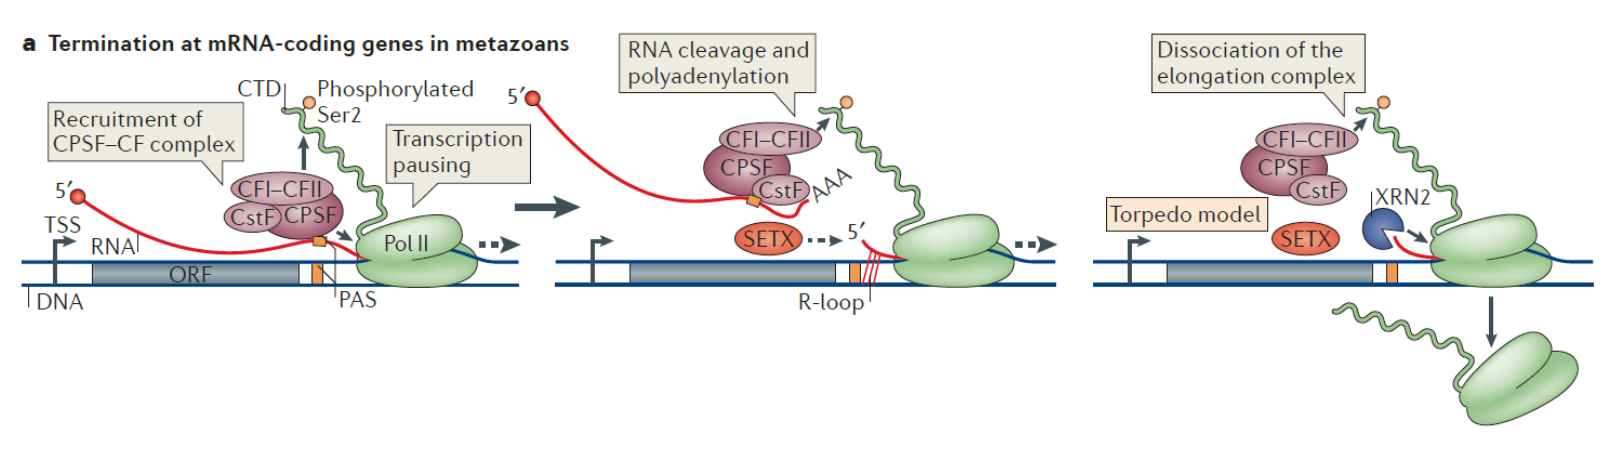
\includegraphics[width=0.5\textwidth]{../_resources/Screenshot_2022-10-10_at_10-38-48.png}
\caption{Porrua \& Libri, Nature Review Mol Cell Biol, 2015}
\end{figure}

Porrua \& Libri, Nature Review Mol Cell Biol, 2015

\hypertarget{promoter-reporter-assay}{%
\subsection{Promoter reporter assay}\label{promoter-reporter-assay}}

Since transcription at core promoters can be induced by distal elements, we can perform a promoter reporter assay to investigate which regions actively regulate transcription.

In order to perform the assay, we need to clone the upstream region of a known gene e.g.~GFB. \emph{Cloning vector}: enhancer + CNV (promoter and enhancer)+ multiple cloning sites (\textbf{MCS}) + GFB (coding sequence + polyA site) + OriC + amp.

\begin{enumerate}
\def\labelenumi{\arabic{enumi}.}
\tightlist
\item
  Linearize a plasmid by cutting it with restriction enzyme (HIND) and run it on the gel for extraction
\item
  Ligation
\item
  Transformation through heat shock
\item
  Integration screening (check amp resistance)
\end{enumerate}

After cloning, we transfect the compound in cells. GFB will be barely detectable. We could start again with a longer sequence and clone it in from of GFB, but it would still be undetectable. It is required to employ a longer gene for observing signal. By playing with deletions, we understand that we only need small regions: 100 bp at TSS and a proximal enhancer region.

\begin{figure}
\centering
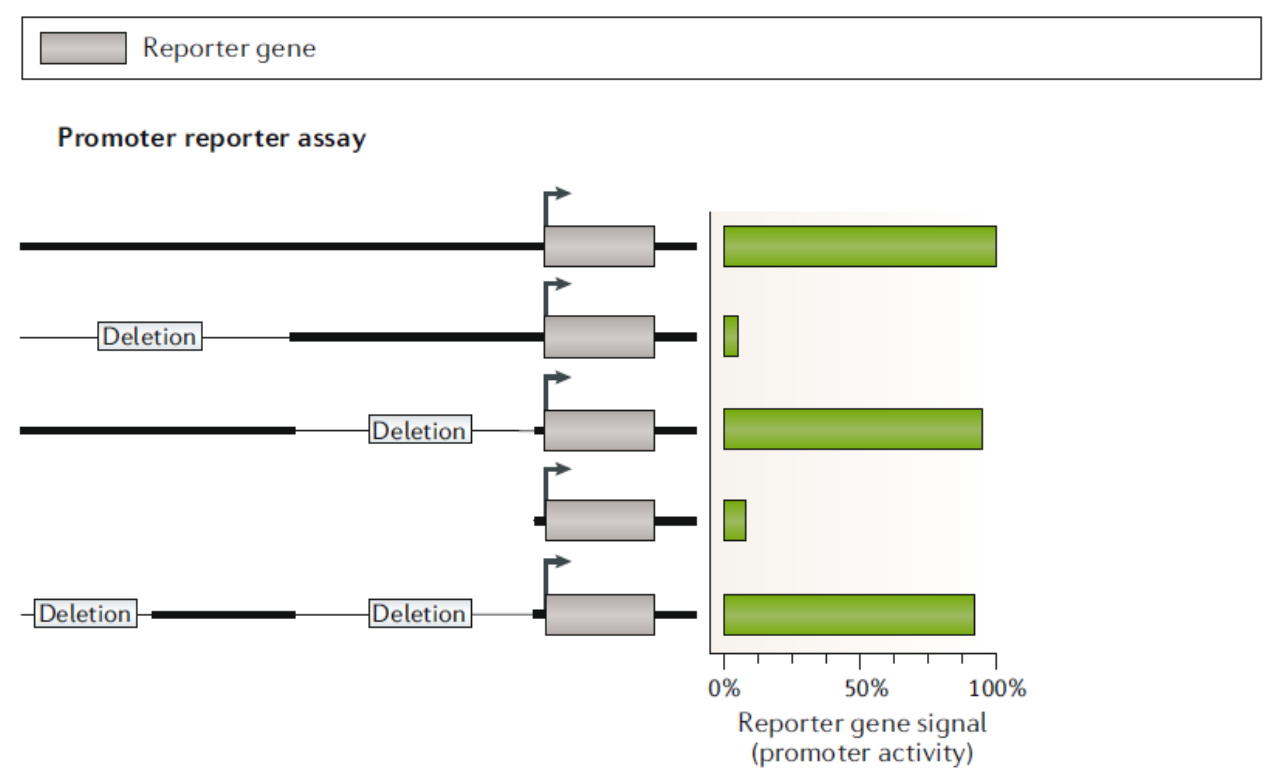
\includegraphics[width=0.5\textwidth]{../_resources/Screenshot_2022-10-10_at_10-45-54.png}
\caption{Anderson \& Sandelin, \emph{Nature Review Gen}. 2019}
\end{figure}

Anderson \& Sandelin, \emph{Nature Review Gen}. 2019

The enhancer can be hundreds of kilobases away from the promoter, could be upstream or downstream, even in introns. In order to check if a gene is an enhancer we need to place it around a reporter gene with different combinations.

\begin{itemize}
\tightlist
\item
  \emph{Core promoter}: sequence that enables to initiate transcription (immediate vicinity of a TSS) by docking the pre-initiation complex (PIC)
\item
  \emph{Promoter}: refers to a sequence which can autonomously drive high levels of productive transcription (proximal enhancer + core promoters)
\item
  \emph{Enhancer}: distal element. The enhancer can be transcribed, but the mRNA is not stable and not codifying for protein.
\end{itemize}

\hypertarget{promoter-types}{%
\subsection{Promoter types}\label{promoter-types}}

Not all promoters have a TATA box, we have 3 different kinds of promoters:

\begin{enumerate}
\def\labelenumi{\arabic{enumi}.}
\tightlist
\item
  \textbf{Type I ('adult')}: TATA box and sharp TSS. No CpG, nucleosomes are not well positioned $\rightarrow$ minority of promoters. Tissue-specific expression.
\item
  \textbf{Type II ('ubiquitous')}: no TATA box and CpG islands. Broad TSS, ordered nucleosome configuration.
\item
  \textbf{Type III ('developmentally regulated'):} featured by polycomb regulation, large CpG islands extending into the body of gene.
\end{enumerate}

\begin{figure}
\centering
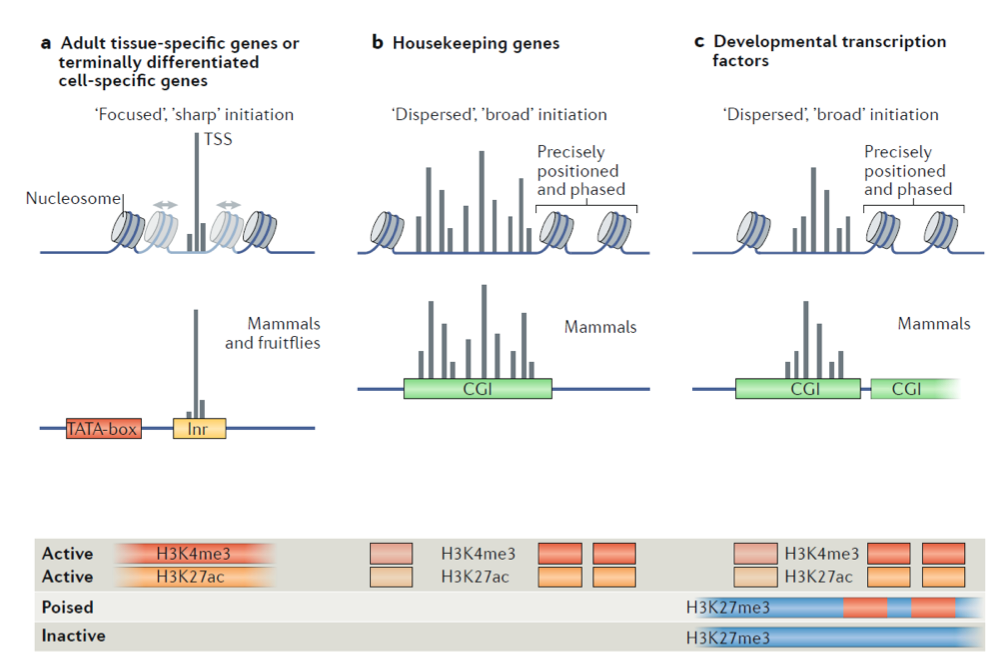
\includegraphics[width=0.5\textwidth]{../_resources/Screenshot_2022-10-05_at_10-05-59.png}
\caption{Lenhard \emph{et al., Nature Rev Cancer} 2012}
\end{figure}

Lenhard \emph{et al., Nature Rev Cancer} 2012

\hypertarget{transcription-factor-binding}{%
\subsection{Transcription factor binding}\label{transcription-factor-binding}}

Most of the times, TFs require co-factors and direct binding; sometimes the \emph{effector domain} can be either a ligand-binding domain or PPI domain.

TFs cooperate and synergize to gain access to their binding sites. For instance, factor A can bind alone to the unwinded first part, then B binds. In general we can observe:

\begin{itemize}
\tightlist
\item
  passive cooperativity
\item
  TF-TF interactions
\item
  enhanceosome model
\end{itemize}

Most TF binding occurs in clusters (\textless1kb) on nucleosome depleted regions. Regulatory networks are usually created with the same TF regulating different genes depending on other TF and cofactors availability.

\textbf{Pioneer TFs} are able to access their own binding sites independently of nucleosome/chromatin binding. For instance, \textbf{FoxA} HTH domain is really similar to H1 linker histone. HTH binds DNA minor groove: it has a trans activator domain and it is able to bind core histone. Once pioneer TF bind, they are able to pull DNA from the nucleosome creating a more accessible stretch. Examples:

\begin{itemize}
\tightlist
\item
  SOX2 exposes DNA for OCT4 $\rightarrow$ \emph{sequential binding mechanism} for recruiting multiple TFs\emph{,} rather than simultaneous
\item
  FoxA1 enables Estrogen Receptor alpha recruitment
\end{itemize}

Other mechanisms we can observe are the recruitment of acetylases e.g.~p300 to enhance nucleosome destabilization.

Transcription is dynamically regulated but not constantly occurring. The core promoter will accomodate a number of pol II, which will then transcribe (burst). Different core promoters can have a different burst size. Enhancers do not change this size (which is given by promoter structure), but increase the number of bursts per time.

\begin{figure}
\centering
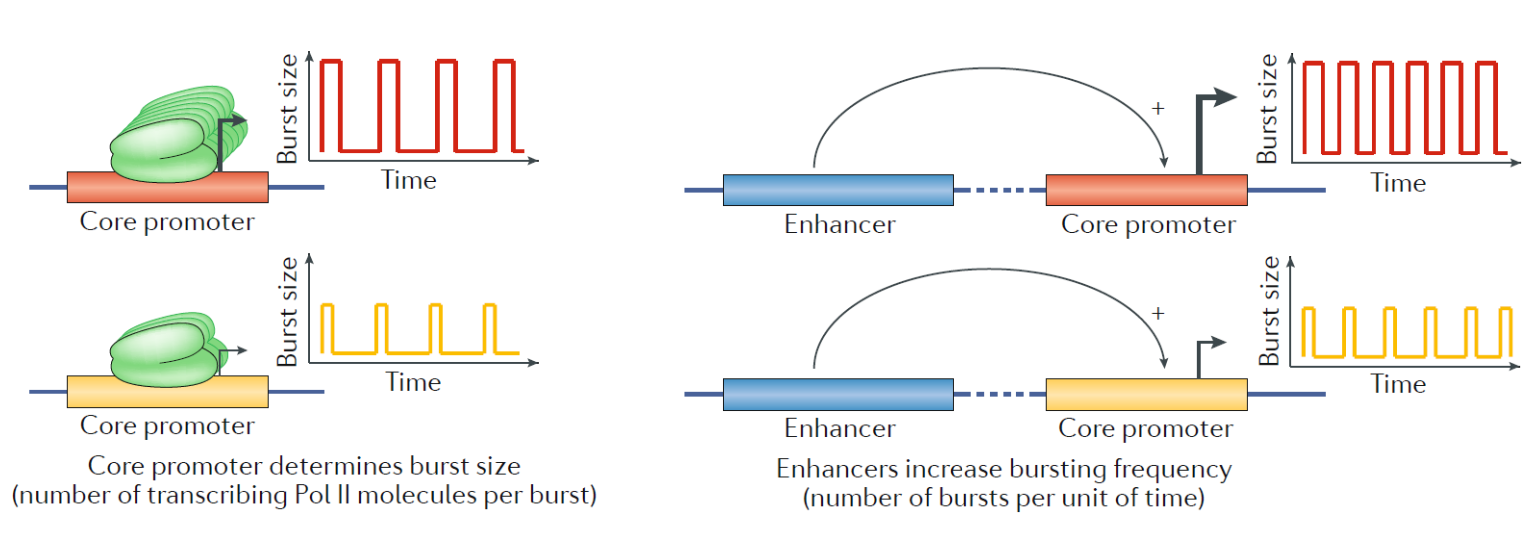
\includegraphics[width=0.5\textwidth]{../_resources/Screenshot_2022-10-10_at_10-50-43.png}
\caption{Haberle \& Stark, \emph{NatRevMolCelBiol.} 2018}
\end{figure}



    \graphicspath{{chapters/_resources/}}

\chapter{Enhancer regulation}



\hypertarget{tcic-1}{%
\section{5 - TCiC (1)}\label{tcic-1}}

Enhancer regulation is controlled by specific transcription factors with a DBD. Most of the times, TFs interact with PIC through co-factors. In particular, the Mediator is a key co-activator complex of RNA pol II transcription regulation.

\hypertarget{mediator-complex}{%
\subsubsection{Mediator complex}\label{mediator-complex}}

The Mediator complex is a multi subunit complex, composed of almost 30 subunits. CDK8 is the only module with enzymatic activity.

\begin{figure}
\centering
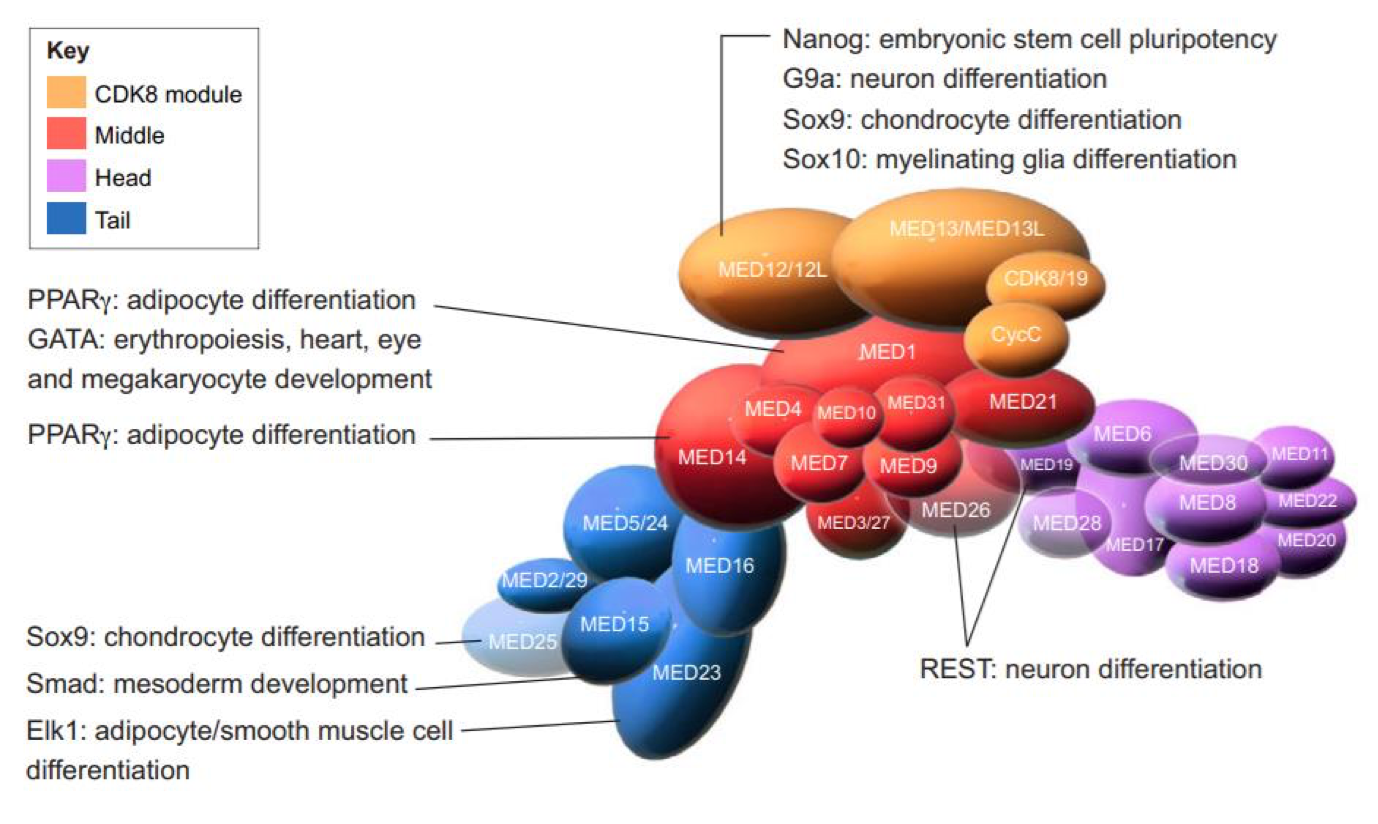
\includegraphics[width=0.5\textwidth]{../_resources/Screenshot_2022-10-07_at_10-47-50.png}
\caption{Screenshot 2022-10-07 at 10.47.50.png}
\end{figure}

The Mediator complex can interact with hundreds of TFs and integrate their function, allowing cooperation and regulation of multiple sites in enhancer regions. Examples: SOX,c-Myc,\ldots{}

Since the Mediator is a multi-subunit structure, a conformational change in one subunit propagates to the whole complex.

The interaction with Pol II prevents the catalytic interaction: the core mediator has mutually exclusive interactions.

\begin{figure}
\centering
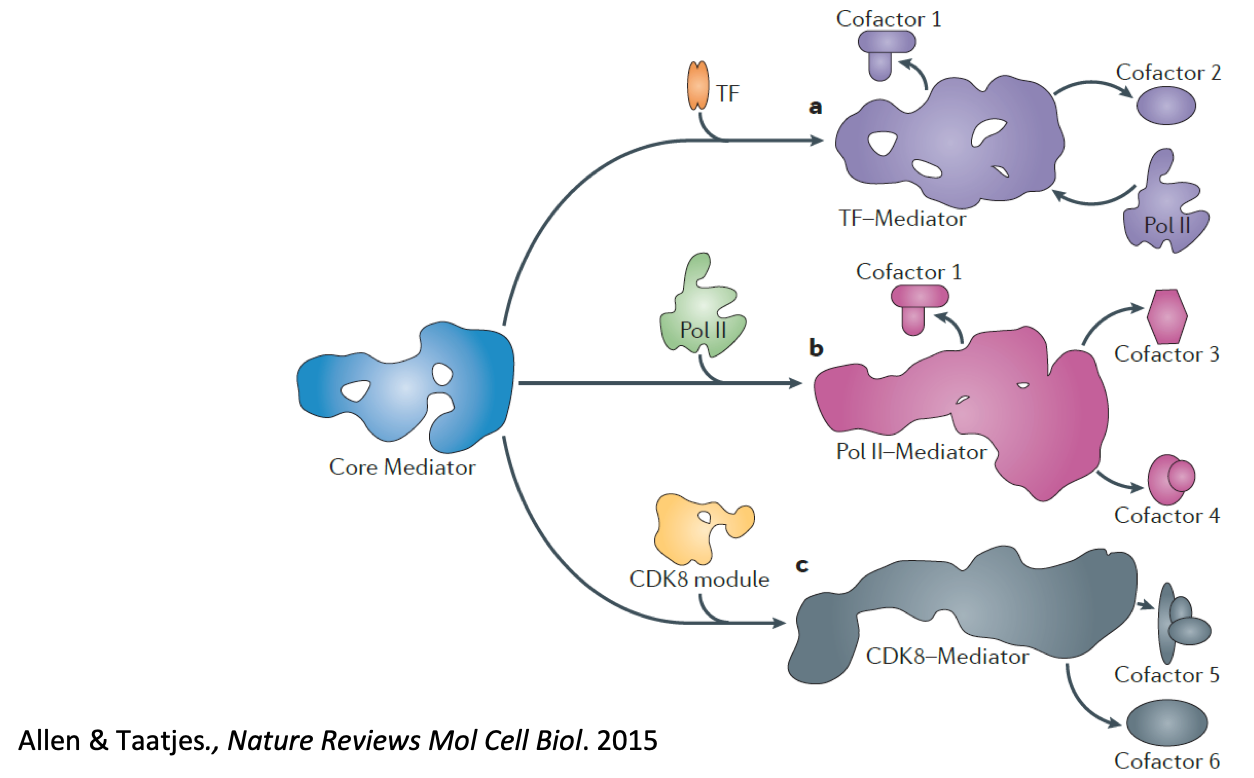
\includegraphics[width=0.5\textwidth]{../_resources/Screenshot_2022-10-07_at_10-50-30.png}
\caption{Screenshot 2022-10-07 at 10.50.30.png}
\end{figure}

The Mediator functions as a bridge between the TFs bound to the enhancers and the PIC at core promoters; DNA looping involves \emph{cohesins} (circle DNA). The interaction with enhancers occurs first and is more stable than the core promoter one.

\begin{figure}
\centering
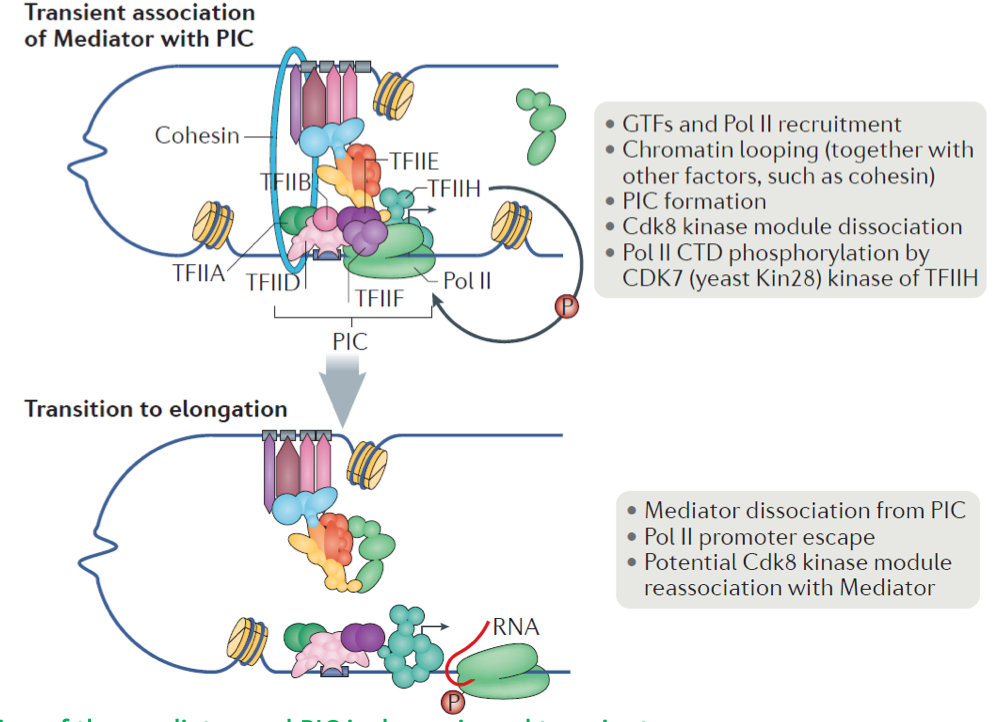
\includegraphics[width=0.5\textwidth]{../_resources/Screenshot_2022-10-07_at_10-54-13.png}
\caption{Soutourina\emph{, Nature Review Mol Cell Biol.} 2018}
\end{figure}

Soutourina\emph{, Nature Review Mol Cell Biol.} 2018

The Mediator stimulates transcription at several levels: assembly of the PIC, chromatin organization, transcription elongation, nucleosome displacement at TATA-box promoters. After Pol II promoter escapes, the Mediator interacts with Cdk8 to activate pause release. The Mediator presence at TATA regions inversely correlates with nucleosome occupancy : indeed, it is able to bind acetylated histones and interact with chromatin remodelling complexes contributing in histone eviction.

The Mediator has been defined as GTF (general TF), however it preferentially associates with enhancers and its occupancy at core promoters is generally low and transient.

Once the Mediator is interacting with the PIC, CDK8 is displaced; afterwords, the Mediator is able to recruit it again to activate Cdk9, allowing the pausing mechanism.

\begin{figure}
\centering
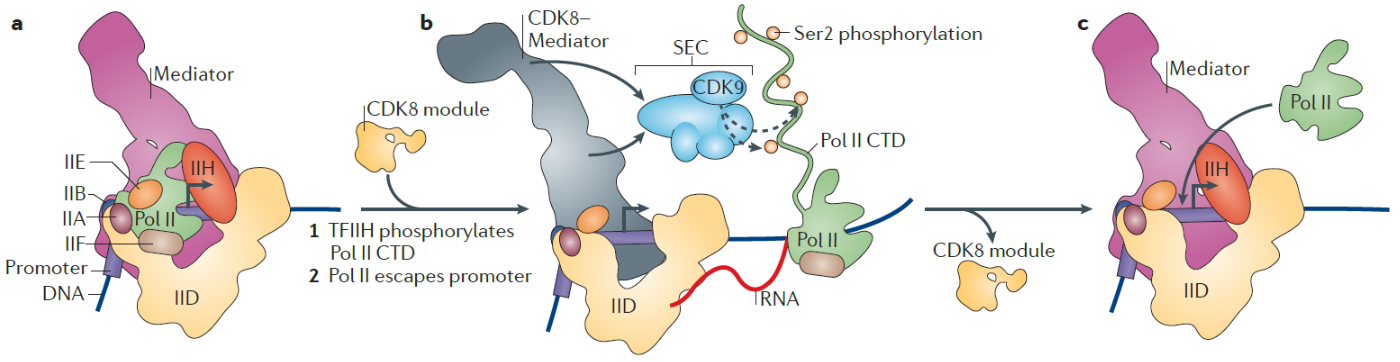
\includegraphics[width=0.5\textwidth]{../_resources/Screenshot_2022-10-10_at_11-03-13.png}
\caption{Allen and Taatjes, \emph{Nature Reviews Mol Cell Biol}. 2015}
\end{figure}

Allen and Taatjes, \emph{Nature Reviews Mol Cell Biol}. 2015

The multi-subunit and modular structure of the Mediator enables to respond to multiple signalling cascades activating transcription. Different subunits can be engaged in PPIs; we are interested in many of them, in particular oncogenes usually interact with the mediator.

\hypertarget{wnt-signalling-pathway}{%
\subsection{Wnt signalling pathway}\label{wnt-signalling-pathway}}

Wnt signalling pathway is a relevant pathway for morphogenesis and embryonic development, as well as adult tissue homeostasis. Its activation is associated with cell proliferation and cell renewal.

The pathway occurs at a plasma membrane, where \textasciitilde20 ligands interact among themselves and with a core receptor (either LRP5 or LRP6). A

\begin{itemize}
\tightlist
\item
  Off: XIN1 forms a \emph{destruction complex} with APC, CK1, GSK, which recruits \textbf{$\beta$  -catenin}, a relevant co-activator. The activation is performed through phosphorylation or ser and threonine residues, which will then recruit btrCP ubiquitinylase and lead to b-cat degradation.
\item
  On: when Wnt is present, the complex is sequestered and therefore b-catenin is not phosphorylated and ubiquitinylated, it remains present in the cell. Among target genes, AXIN2 promotes the recruitment and formation of distraction complex, others are plasma membrane proteins which promote \emph{endosome mediated degradation} of WNT.
\end{itemize}

\begin{figure}
\centering
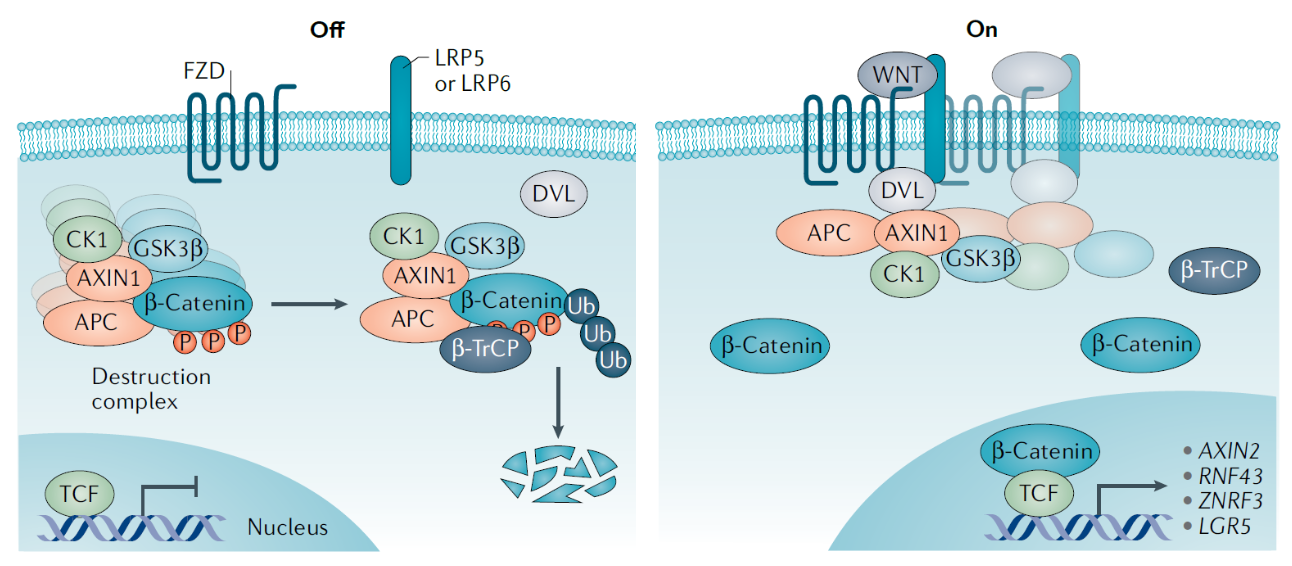
\includegraphics[width=0.5\textwidth]{../_resources/Screenshot_2022-10-10_at_11-03-55.png}
\caption{Bugter \emph{et al., Nature Review Cancer}, 2021}
\end{figure}

Bugter \emph{et al., Nature Review Cancer}, 2021

\begin{figure}
\centering
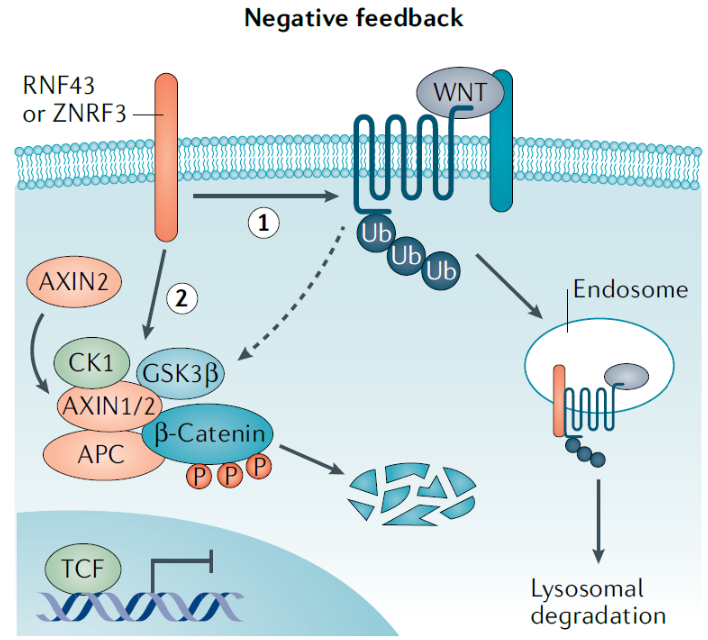
\includegraphics[width=0.5\textwidth]{../_resources/Screenshot_2022-10-10_at_11-04-14.png}
\caption{Screenshot 2022-10-10 at 11.04.14.png}
\end{figure}

Wnt is synthesized in the endoplastic reticulum, lipid modified and released from cells through EVs (or can remain attached to membrane of secreting neighbouring cells). It can spread and reach different sites.

Excessive $\beta$  -catenin activity in cancer can occur due to:

\begin{itemize}
\tightlist
\item
  inactivating mutations in members of the destruction complex
\item
  negative feedback pathway (RNF43 or ZNRF3) and activating mutations $\beta$  -catenin
\end{itemize}

Genetic alterations in the WNT pathway occur in most cancer types with some components of the pathway showing tissue specificity. All WNT mutations converge in enhancing $\beta$  -catenin activity, although with different extent, and cooperate with other driver mutations to promote tumorigenesis. Mutation are considered early (APC) or late (RNF43) events and associate with different tumor subtypes. APC mutant tumor leads to many clinical features: depending on the function and position in the pathway of the gene, the downstream effect can be very different.

In absence of $\beta$  -catenin (Wnt pathway off), TLE and HDAC bind TCF and stop transcription. $\beta$  -catenin subcellular translocation is presumed to function thanks to the binding of adaptor proteins. $\beta$  -catenin needs to interact with different TFs, among which TCF family members are the most common and expressed in different forms. They all recognize the same binding site. In particular, different isoforms of TCF7 and LEF1 are highly expressed in colorectal cancer.

\hypertarget{ux3b2-catenin-structure}{%
\subsubsection{$\beta$  -catenin structure}\label{ux3b2-catenin-structure}}

$\beta$  -catenin structure acts as a binding platform for numerous interactions. It is composed of 781 aa residues in humans and divided in:

\begin{itemize}
\tightlist
\item
  central highly repetitive sequence with \emph{Armadillo sequence} important for nuclear activity.
\item
  Helix-C conserved structure close to CTD
\item
  C-terminal transcription activator domain (CTTA)
\end{itemize}

Key interactors: E-cadherin and A-cathenin → structural function, focal adhesion. Decrease in E-cadherin is found in EMT. E-cadherin cad is stabilized by $\beta$  -catenin, therefore with low levels of $\beta$  -catenin we observe an E-cadherin decrease in ETM.

The function of $\beta$  -catenin, both structural and signaling, is regulated by post-translational modifications.

RNA pol II is also loaded on inactive genes; to foster elongation we require $\beta$  -catenin, which can recruit PAF1 complex. The majority interact with the CTTA domain, which serves as a binding platform or trans-activation domain.

\begin{figure}
\centering
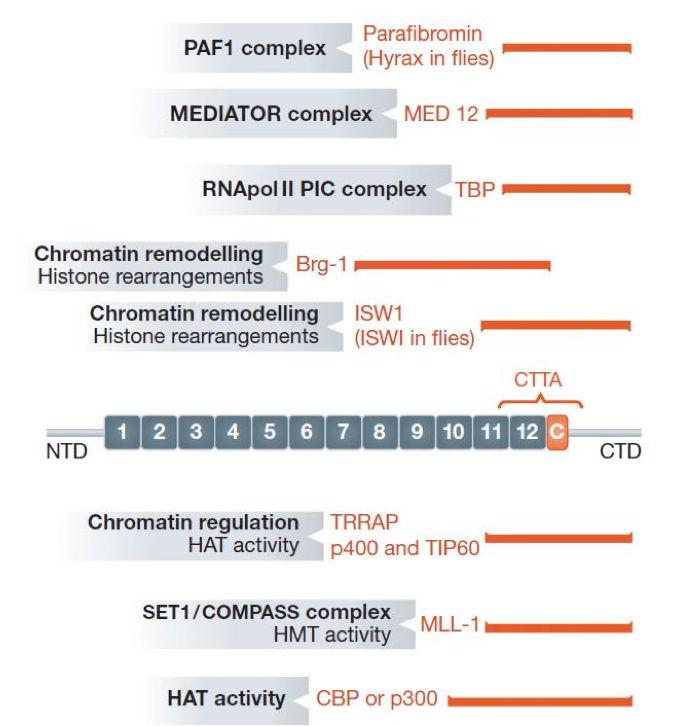
\includegraphics[width=0.5\textwidth]{../_resources/Screenshot_2022-10-07_at_11-52-13.png}
\caption{Valenta \emph{et al., EMBO J.} 2012}
\end{figure}

Valenta \emph{et al., EMBO J.} 2012

\begin{figure}
\centering
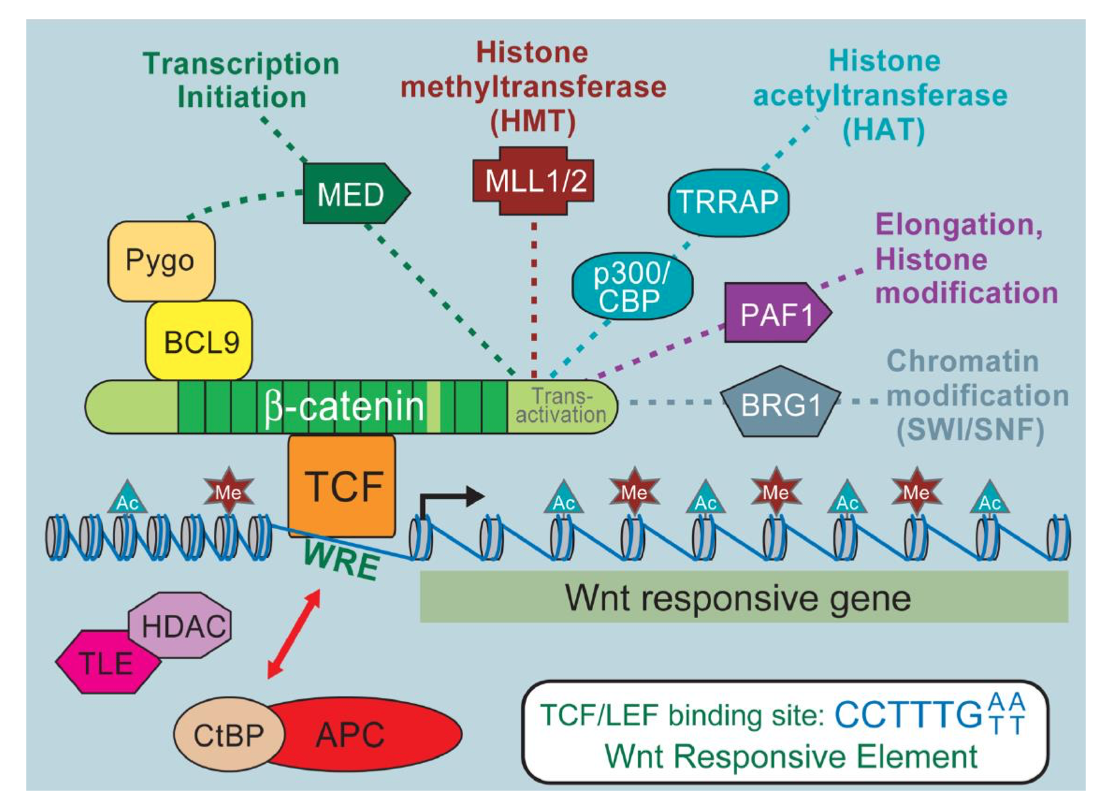
\includegraphics[width=0.5\textwidth]{../_resources/Screenshot_2022-10-07_at_11-52-58.png}
\caption{McDonald \emph{et al., Dev Cell}, 2009}
\end{figure}

McDonald \emph{et al., Dev Cell}, 2009

\hypertarget{the-canonical-wntux3b2-catenin-pathway-is-crucially-involved-in-colorectal-cancer}{%
\subsubsection{\texorpdfstring{\textbf{The canonical Wnt/$\beta$  -catenin pathway is crucially involved in colorectal cancer}}{The canonical Wnt/$\beta$  -catenin pathway is crucially involved in colorectal cancer}}\label{the-canonical-wntux3b2-catenin-pathway-is-crucially-involved-in-colorectal-cancer}}

The \textbf{APC gene} was first identified by being mutated in a hereditary colon cancer syndrome termed familiar adenomatous polyposis. Most cases of sporadic colorectal cancer result from loss of both APC alleles. Loss of APC function leads to the inappropriate stabilization of $\beta$  -catenin and the formation of constitutive complexes between $\beta$  -catenin and the intestinal TCF family member TCF7l2/TCF4 Patients with hereditary Axin2 mutations display a predisposition to colon cancer. Aberrant activation of the canonical Wnt/$\beta$  -catenin pathway occurs in almost all colorectal cancers, contributing to their growth, invasion and survival.

\emph{Luciferase reporter genes}: firefly and renilla Luc, of the two only one has a responsive site to TCF. It is a control for the efficiency of transfection.

Let's see which genes are involved in the regulation of $\beta$  -catenin through RNAi in DLD1 cells: 34 genes are necessary for $\beta$  -catenin activity and 166 candidate genes are necessary for HCT116 cells proliferation. By merging the two groups, we can identify a set of 9 potential regulators of colon cancer proliferation and $\beta$  -catenin activity: CDK8, CSK1G3, CSNK1E, DKC1, MAP3K14, MLLT7, PLK4, TAOK1 and ZAK.

Genome wide analysis of chromosome copy number alterations (CNA) in human CRC biopsies revealed amplification of chr. 13 region including CDK8. Immunohistochemical analysis of CDK8 expression in the same 50 specimens revealed elevated protein levels in 26\% colon cancer samples, including those that showed CDK8 CN gain {[}the brownish colour in IHC indicates that CDK8 expression increases{]}.

\begin{figure}
\centering
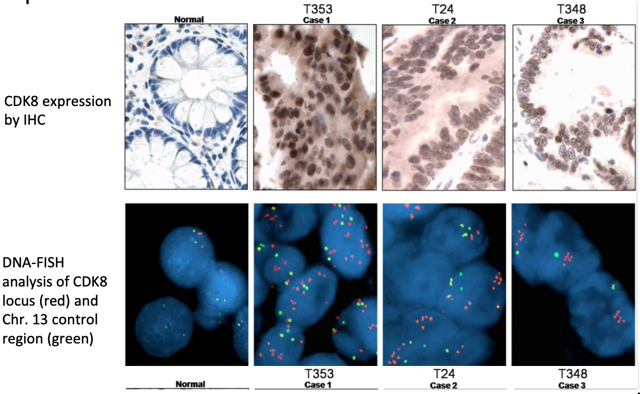
\includegraphics[width=0.5\textwidth]{../_resources/Screenshot_2022-10-10_at_12-23-14.png}
\caption{Firestein \emph{et al., Nature} 2008}
\end{figure}

Firestein \emph{et al., Nature} 2008

These observations indicate that CDK8 is amplified and overexpressed in a substantial fraction of colon cancers. In particular, CDK8 action is not a passenger effect, it is a \emph{driving proliferation}. There is a huge difference from in vitro and in vivo tumor setting: in order to obtain more suitable experiments, we can look at the transforming potential (as not all proliferating cells are necessarily tumor cells). If we combine $\beta$  -catenin in catalytically dead CDK8 we drop the affect, but it is not completely abolished - as $\beta$  -catenin can bypass the need engaging interactions with others.

\textbf{Main conclusions of the article}

\begin{itemize}
\tightlist
\item
  CDK8 acts as an oncogene in a substantial fraction of colorectal cancers
\item
  CDK8 kinase activity is essential to regulate $\beta$  -catenin dependent transcription and transformation
\item
  CDK8 acts in part by co-activating $\beta$  -catenin driven transcription in colon cancer with high CDK8 expression and $\beta$  -catenin activity
\end{itemize}

\underline{Therapeutic interventions that target CDK8 kinase activity may be of clinical value in colorectal cancer}

Almost all Mediator subunits have been found to be mutated/deregulated in a huge list of cancers e.g.~MED12 subunit in prostate cancer.

\hypertarget{transcriptional-control-in-cancer}{%
\section{6- Transcriptional Control in Cancer}\label{transcriptional-control-in-cancer}}

\href{https://www.notion.so/TCiC-08701b51973a4b22a16e226a1fbd7e9b}{TCiC}

\hypertarget{crepp300}{%
\section{CREP/p300}\label{crepp300}}

CREB-binding protein (CBP) and p300 is a heavily regulated TF. Differently from the Mediator, it is a monomer and has several trans-activation domain, which enable it to interact with TF and PIC. It has histone acetyltransferase activity (HAT) or lysine acetyltransferase activity (KAT). Chromatin will be modified by increasing accessibility and also TF regulation.

\hypertarget{crepp300-structure}{%
\subsubsection{CREP/p300 structure}\label{crepp300-structure}}

\begin{itemize}
\item
  4 transactivation domains
\item
  histidine rich or glutamine rich regions.
\item
  Zinc fingers domain for PPIs
\item
  bromodomain and PHD interact with histones
\item
  lysine acetyltransferase domain (HAT)

  \begin{figure}
  \centering
  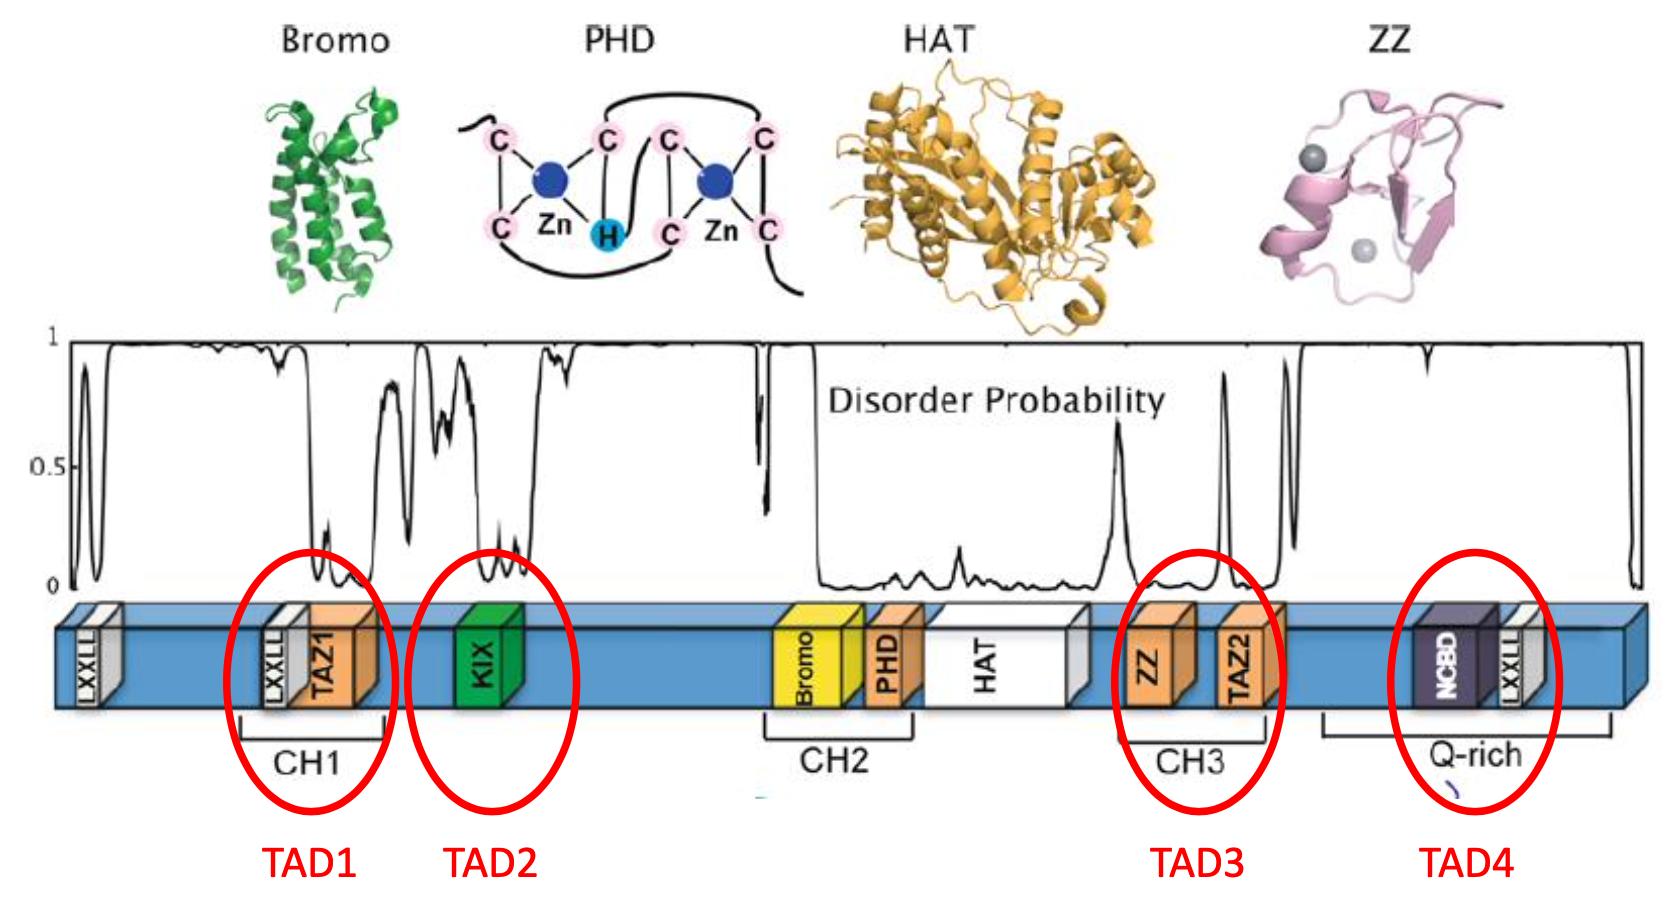
\includegraphics[width=0.5\textwidth]{../_resources/Screenshot_2022-10-12_at_08-56-06.png}
  \caption{Wang \emph{et al., Cell Mol Life Sci.} 2013}
  \end{figure}

  Wang \emph{et al., Cell Mol Life Sci.} 2013
\end{itemize}

There are no intrinsically disordered regions, they fold after interacting with id proteins.

Note that among CBP/p300 binding partners we find both oncosuppressor genes and oncogenes, as well as co-factors.

TF interactions are mediated by TADs. There is a combined interaction among multiple TFs and CBP, enabling the integration of the function of several TFs. The interaction with enhancers does not necessarily correlate with transcription activation; only when the appropriate number and identity is recruited on the enhancer, it becomes functional.

CBP/p300 levels in cells are limiting and different genomic sites or pathways compete for their activity.

In the case of p300, we observe the \emph{co-binding mechanism} with common cofactors or common complexes (transcriptional synergy).

Co-activators facilitate transcription by numerous mechanisms:

\begin{itemize}
\tightlist
\item
  Adaptors function: bridging TFs to the PIC, recruitment of polII to core promoters, recruitment of chromatin remodelling and modifying enzymes to core promoters
\item
  Scaffolding function: facilitating protein-protein and protein-DNA interactions, promoting/stabilizing PIC formation
\item
  Enzymatic activities: Kinase (mediator), KAT (CBP/p300) targeting histones, TFs and non-TF proteins (acetylation of P-TEFb enhances its activity).
\end{itemize}

Their activity can vary from gene to gene depending on TF involved and regulated by PTMs and chromatin accessibility.

In particular, CBP/p300 can regulate pro-proliferative pathways, e.g., cell cycle regulation.

\begin{figure}
\centering
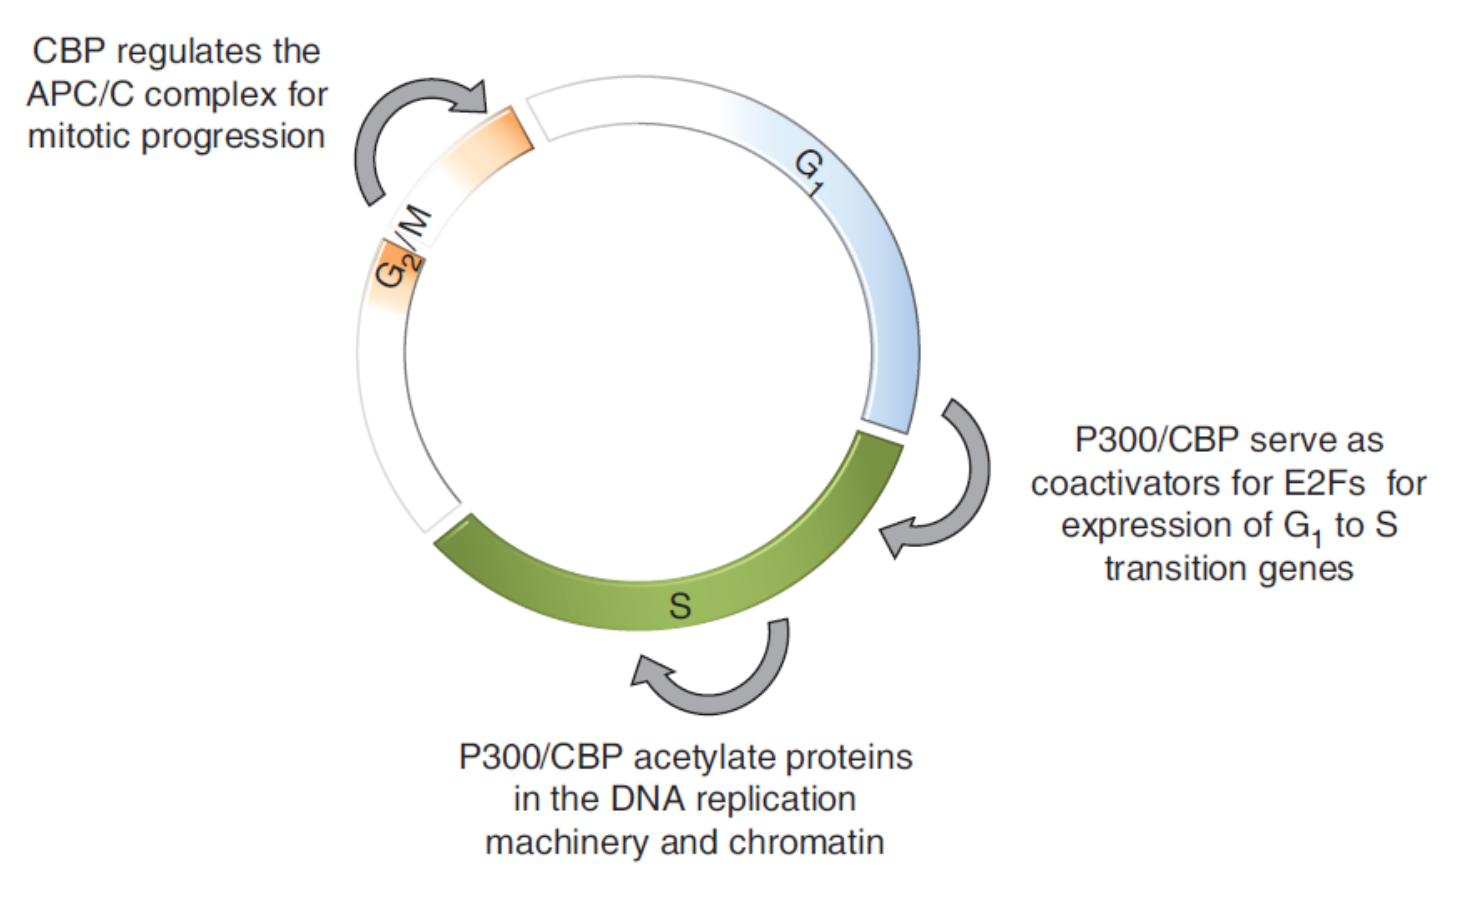
\includegraphics[width=0.5\textwidth]{../_resources/Screenshot_2022-10-12_at_09-01-27.png}
\caption{Screenshot 2022-10-12 at 09.01.27.png}
\end{figure}

Indeed, CBP and p300 gene are frequently mutated in cancer - mutually exclusive. Most are missense mutations (single nucleotide), some deletions and insertions. Mutation hotspots are found at the catalytic domain (KAT). We always need to consider the context of genetic instability characterizing cancer: depending on which signal is activated/repressed, a particular mutated form can either excerpt proliferative or oncosuppressor activity {[}often loss of heterozygosity{]}.

The many functions of CBP/p300 can be differentially exploited in cancer depending on the context, leading the CBP/p300 proteins to act as oncosuppressors or oncogenes. Depending on cellular identity, dysregulated pathways and transcription rewiring, cancer cells may select for the CBP/p300 alterations most advantageous for survival and growth.

\hypertarget{tssa-rnas-transcription}{%
\subsection{\texorpdfstring{\textbf{TSSa-RNAs transcription}}{TSSa-RNAs transcription}}\label{tssa-rnas-transcription}}

Transcription by RNA Pol II is often thought to occur unidirectionally, however we also observe an enrichment of transcripts in the opposite direction with respect to forward transcription. TSSa-RNAs (TSS antisense) surround promoters in nonrandom and divergent orientations. Sense TSSa-RNAs map downstream of the associated promoter, overlapping genic transcripts and peaking in abundance between +0 and +50 nt downstream of the TSS. Antisense TSSa-RNAs peak between nucleotides --100 and --300 and can range from 20 to 90 nt (detected by Northern blot). The mere fact of having high abundance of TF can recruit pol II, which can act \emph{spuriously}: it not only transcribes following the functional direction, but also in the opposite direction (with different pre-initiation complexes).

It is presumed that these small transcripts are abortive transcription tentative; stalling can occur if RNA is not properly processed e.g.~no recruitment of cap proteins, so after degradation and when RNA pol II is displaced, a short sequence (which was protected by pol II) remains at the site. In general, there is a bias towards the directionality of these transcripts, confirming the previous hypothesis; highly expressed genes all have TSSa-RNA.

Although divergent transcription initiation is widespread and might have functions, productive elongation by RNAP II occurs primarily unidirectionally, downstream of TSSs. Promoter upstream transcripts (PROMPTs) are longer than TSS-a and are more stable, while PASRs overlap on the TSS.

Different families of noncoding RNAs are transcribed at promoters of protein coding genes:

\begin{itemize}
\tightlist
\item
  Transcription start-site-associated (\textbf{TSSa}) RNAs are short transcripts (18-24 up to 90bp), do not overlap TSS, sense or antisense of the mRNA
\item
  Promoter associated short transcripts (\textbf{PASRs}): capped bidirectional short RNA (20- 100nt long) that overlap TSS
\item
  Promoter upstream transcripts (\textbf{PROMPTs}): capped bidirectional ncRNAs, map upstream of active promoters (-500 and -2000 from TSS)
\end{itemize}

Potential functions
\begin{itemize}
\item Help modulating chromatin structure due to the Pol II activity and/or binding with chromatin i.e.~help sustaining nucleosome free regions
\item  Noncoding RNAs as precursors for short ncRNA (especially longer ones)
\end{itemize}

{[}RNAse are degraded by the exosome, which is a multi-subunit complex which recognizes uncut RNAse.{]}

\textbf{ENCODE} (Encyclopedia of DNA Elements) has the objective to map all RNAs, which are divided into long and short and by cellular location - either cytoplasmatic or nuclear.

\begin{itemize}
\tightlist
\item
  74.7\% of human genome is transcribed (primary transcripts)
\item
  short RNAs detected:$\sim$160,000 transcripts ( $\sim$40,000 exonic, $\sim$55,000 intronic,$\sim$45,000 intergenic,$\sim$23,000 gene-intergene boundaries)
\item
  long RNA transcripts detected:$\sim$60,000 transcripts from$\sim$19,000 protein coding genes (GENECODE v7); 73,325 transcripts mapping within intergenic regions (also enhancers) and antisense elements (long noncoding RNAs and possible new genes)
\end{itemize}

TSS identified within enhancer regions with transcription proceeding for several kilobases giving rise to \textbf{eRNAs}.

\emph{How can we distinguish enhancers?} By analysing epigenetic marks, TF binding and especially co-factor binding (ChIP-Seq).

Poly(A)- mostly enriched, but also Poly(A), detectable by CAGE hence capped. Transcribed enhancers on average show a significantly different pattern of chromatin modification than non-transcribed ones e.g.~H3K27ac,\ldots{} All the markers are associated with transcription initiations.

In addition to the fact that enhancers need to regulate transcription to allow RNA production, transcription can occur bidirectionally and the enhancer itself can be transcribed.

\begin{itemize}
\tightlist
\item
  \textbf{poised enhancer:} TF bound to the enhancer LDTF (lineage-determinant TF), which is a pioneer TF. We can see some histone modifications for activation, but they are not sufficient to fully activate the promoter. Even pol II can or cannot be recruited, it is not yet acting on a target promoter, but it is active.
\item
  \textbf{active enhancer:} Mediator recruitment, HAT activity, nucleosome remodelling complexes and transcription occurs on the enhancer.
\end{itemize}

Example: the signalling of NFKB TF starts in cytoplasm, it only is shuttled to nucleosome upon a specific signal. Since it is not pioneer TF, it can only bind to poised enhancer → cell-line dependent mechanism.

An active enhancer shows high levels for H3K4me (especially me3), Pol II and Ser5P, H3K27ac, while other elongation markers are less observed. Example of cell-specific regulation: TAL1 TF , oncogene expressed in endothelial cells and erythroid cells, we witness enrichment of H3k4me2 at enhancer sites. Active enhancers associate with chromatin looping.

\hypertarget{properties-of-ernas}{%
\subsubsection{Properties of eRNAs}\label{properties-of-ernas}}

\begin{itemize}
\tightlist
\item
  eRNAs are transcribed from putative enhancer regions characterized by high levels of H3K27ac and the lack of the repressive H3K27me3 mark
\item
  These genomic regions are bound by TFs and associate with transcriptional co- regulators including Mediator, histone acetyltransferase CBP/p300
\item
  eRNA-expressing enhancers are also enriched with PIC
\item
  eRNAs are 50-2000 nt in length and generally exhibit shorter half-lives compared to
  mRNAs and lncRNAs. They are generally not spliced or polyadenylated
\item
  Enhancer transcripts are preferentially enriched at enhancers engaged in chromatin looping with promoters of protein-coding genes and other enhancers, which is a feature correlated with enhancer activity
\end{itemize}

\textbf{eRNAs proposed functions:}

\begin{figure}
\centering
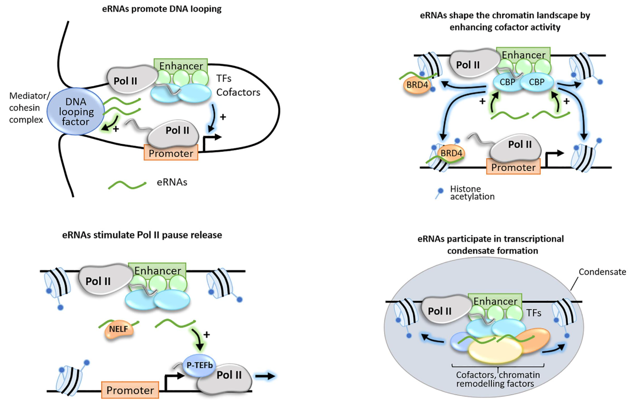
\includegraphics[width=0.5\textwidth]{../_resources/Screenshot_2022-10-12_at_10-00-02.png}
\caption{Studniarek \emph{et al., Trends in Genetics,} 2021}
\end{figure}

Studniarek \emph{et al., Trends in Genetics,} 2021

Last function: Intrinsically disordered proteins → phase separation mechanism. We are enriching the density of enzymes in a particular region.

In particular, eRNA can promoter chromatin remodelling recruitment to reach appropriate configurations for chromatin at TSS.

\hypertarget{assessing-whether-the-crc-8q24-risk-region-acts-as-an-enhancer}{%
\subsubsection{\texorpdfstring{\textbf{Assessing whether the CRC 8q24 risk region acts as an enhancer}}{Assessing whether the CRC 8q24 risk region acts as an enhancer}}\label{assessing-whether-the-crc-8q24-risk-region-acts-as-an-enhancer}}

Most mutations in cancer are SNPs and mainly occur outside of coding regions. Driver mutations are commonly found at coding regions, but also outside of it. One way in which we can analyze non-coding region is assessing the frequency of mutation for a region. In 2007, two different studies found that some SNPs located in 8q24 were highly associated with colorectal cancer.

In particular, the rs6983267 SNP G allele (over T allele) on 8q24 associates with increased risk of colorectal cancer. Homozygosity for the risk G allele in cancer increases CRC risk 1.5 folds.

One way to study non-coding SNP is to understand whether it can be a regulatory region:

\begin{enumerate}
\def\labelenumi{\arabic{enumi}.}
\tightlist
\item
  ChIP-Seq: the risk locus with G shows an enrichment in RNAP II, methylation and p300
\item
  Reporter assay: 1.5 kb long region including the risk allele can function as an enhancer. The G risk allele shows increase reporter activity than the WT allele for the risk allele. It is not a 10 fold difference, suggesting it is not a driver mutation.
\end{enumerate}

Epigenetic and reporter assay data indicate that the CRC risk allele functions as an enhancer.
The rs6983267 SNP is located with a \textbf{TCF} consensus binding site (A/T)(A/T)CAA(A/T)GG. This site is not an exact consensus sequence, but if we have a G on the last position we achieve a higher affinity. By performing ChIP on TCF4, the peak for G allele is higher than T. There is no gene for hundreds of kbs, but if we move forward we find Myc. Since TCF4 is an effector of Wnt pathway and Myc is a beta-catenin target, the SNP can be placed in Myc enhancer region. Instead, no association between MYC mRNA expression and CRC risk allele was identified in either normal colon or tumor samples. However, 3C experiments show a physical interaction between the risk allele and MYC promoter was detected in CRC lines but not fibroblasts.

Conclusions:

\begin{itemize}
\tightlist
\item
  The CRC risk locus shows enhancer-like functions in CRC cell lines
\item
  The CRC risk allele interacts with TCF4
\item
  This locus physically interacts with the MYC promoter
\end{itemize}

Hypothesis: the rs6983267 risk allele may regulate MYC during tumorigenesis

Another article from 2009:

Computational approach predicts that the rs6983267 would impact TCF4 binding site, since a change from T to G is predicted to considerably increase the affinity for TCF4 binding. They use a different approach to verify whether TCF4 is interacting with the risk region.

EMSA: in vitro incubation of recombinant proteins (oligonucleotide of interest with radioactive mark). Run electrophoresis: TCF4 with its own sequence, unrelated sequence and SNP alleles sequence. TCF4 can bind the risk allele G, much less affinity for T allele.

Activation of the WNT pathway through GSK3B inhibition indicates WNT responsive enhancer activity. Reporter assay to obtain a biological readout of the process: the entire site is required for the interaction and should not be further mutated. The risk G allele shows 1.5 fold increase in WNT responsitivity compared to the T allele.

    \graphicspath{{chapters/_resources/}}

\chapter{Chromosome domains and oncogene activation}

\section{Genome organization and transcription regulation}

\subsection{CTCF}
An enhancer can work at very high distance with respect to the gene of interest; this means that enhancers have the possibility to regulate many different promoters, how can enhancer activity be directed to a specific target promoter?

\textbf{\emph{Insulator sequences}} prevent the propagation of enhancers signals along the chromatin fiber through their enhancer blocking function mediated by proteins. Insulator genes are usually found at a region densely distributed with genes. They can act in long distance, do not need specific direction and the sequences are recognized by proteins. The main insulator binding protein is a factor called CCCTC-binding factor (CTCF).

\textbf{CTCF} has a peculiar DBD with 11 zinc fingers; each of them can recognize a short consensus motif. In principle, it could recognize huge regions and be very flexible in recognition capabilities, as combinatorial use of its 11 ZF allows binding to 50bp target sites with high sequence variations. CTCF regulates transcription both positively and negatively and can operate as a transcription factor. At first, it was recognized as a repressive TF: it has the ability to shape the DNA molecules, not merely binding on a site distorting it, and to recruit co-factors.

CTCF is the main \emph{insulator-binding protein} in vertebrates. ChIP shows that CTCF binds thousands of sites in the human genome. We can find it mainly in intergenic regions and introns, as well as promoter regions. There is an extensive overlap of CTCF binding sites among cell lines (12000). The consensus sequence recognized by CTCF is the same among cell lines.

CTCF is enriched at the H3K27me3 domain boundaries (CTCF barrier sites). A larger genomic region was analyzed in different cell lines. Almost no overlap was found in the CTCF barrier sites between CD4T cells and HeLa cells, suggesting that CTCF barriers are cell-type-specific. In some cells the site is at the boundary, in others not.

We now know that heterochromatic marks spread up to insulator sequences, which can be recognized by protein and recruit directly or indirectly chromatin remodelling factors.

Main findings:

\begin{itemize}
\tightlist
\item
  CTCF can bind to the same locus in different cell types
\item
  CTCF binding can separate active and repressed chromatin, functioning as barrier to heterochromatin spreading
\item
  CTCF exerts its barrier ability in a cell type dependent manner
\end{itemize}

The function of CTCF appears to be regulated at least at two levels:

\begin{enumerate}
\def\labelenumi{\arabic{enumi}.}
\tightlist
\item
  binding of CTCF to the target sites.
\item
  binding of interacting proteins, providing its functionality
\end{enumerate}

\hypertarget{cohesin-mediates-transcriptional-insulation-by-ccctc-binding-factor}{%
\subsection{Cohesin mediates transcriptional insulation by CCCTC-binding factor}\label{cohesin-mediates-transcriptional-insulation-by-ccctc-binding-factor}}

CTCF was found to interact with cohesins (composed of SMC3, SMC1, SCC1 and SCC3 subunits), which are essential to maintain sister chromatids connected from S phase to metaphase. Cohesins are loaded on chromosomes during G1, but the function is exerted later on. For achieving anaphase, the ring is cut by securins - regulated by APC.

Cohesin is expressed in differentiated postmitotic cells. We expect that replicating cells express cohesin, as it is heavily required in cell cycle. Pulling down SMC3 in mouse brain we still observe a signal, it is probably linked to an additional function of the complex. During G2 we expect that cohesins are holding together sister chromatids, which instead are absent in G1; the binding site is the same, checked by ChIP-Seq $\rightarrow$ cohesin binds to the same sites independent on cohesion CTCF and cohesion share several binding sites (Figure \ref{fig:chip}).

\begin{figure}
\centering
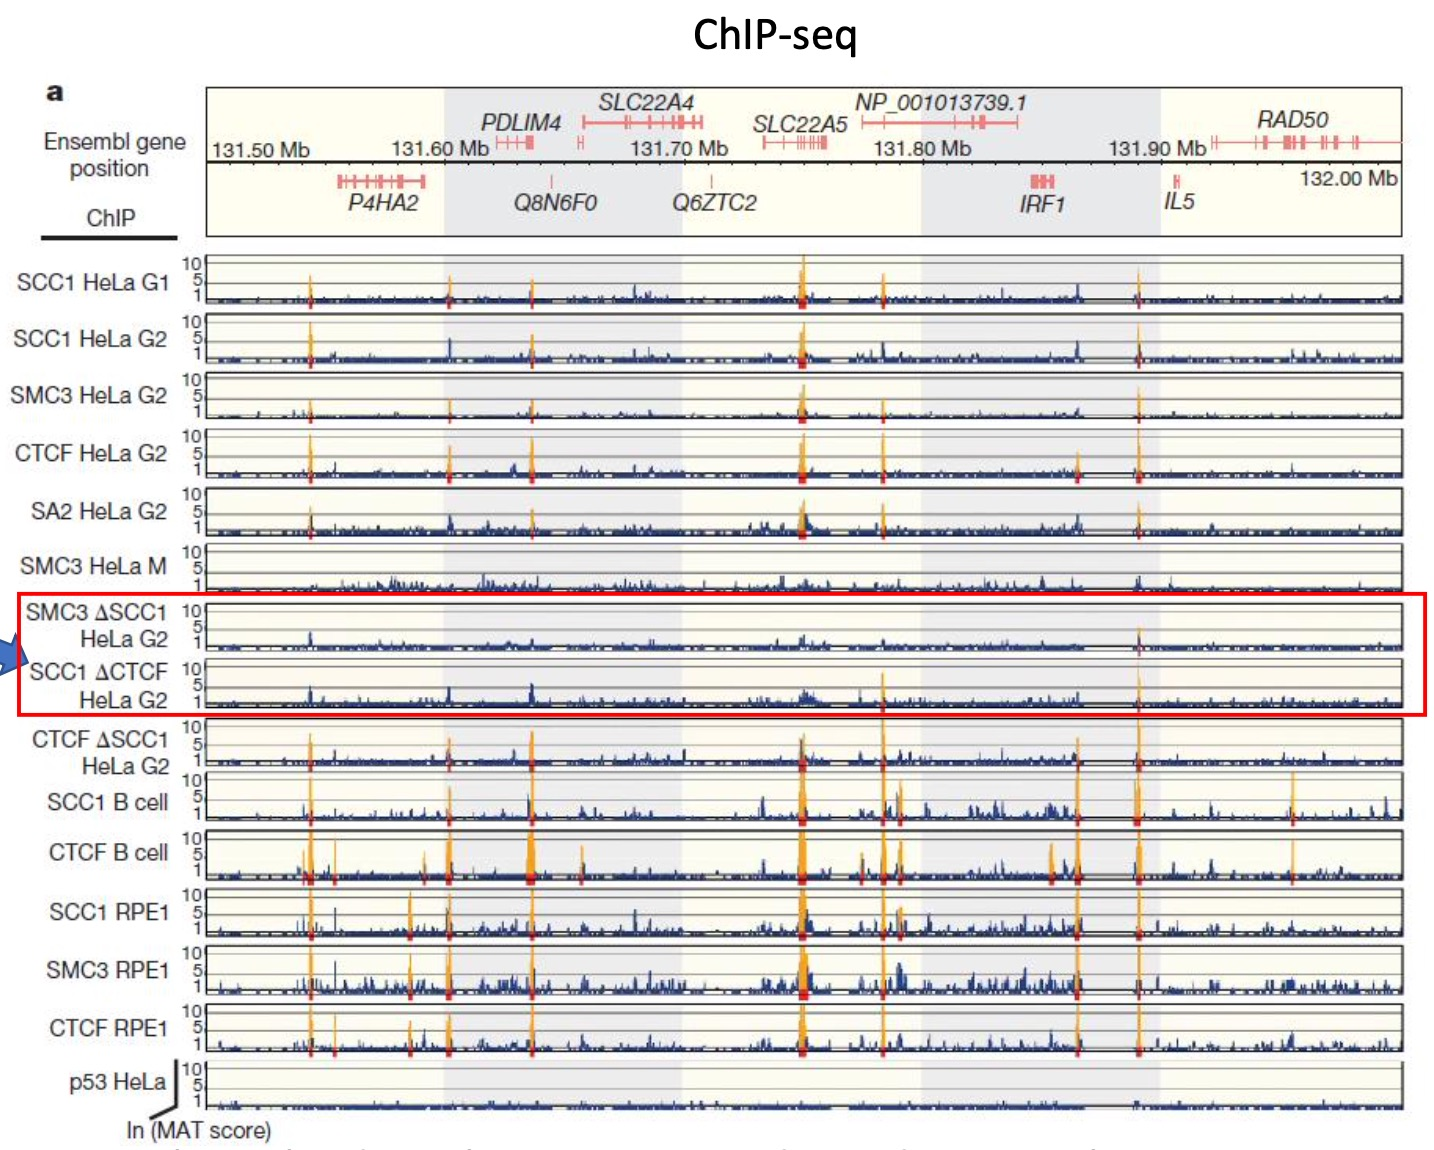
\includegraphics[width=0.5\textwidth]{../_resources/Screenshot_2022-10-14_at_19-51-43.png}
\caption{Yatskevich et al., Annu Rev Genet. 2019}
\label{fig:chip}
\end{figure}

By looking at CTCF KO the binding is lost, as well as SCC1 binding.

Cohesin and CTCF co-occupy thousands of genomic binding sites and share the same consensus sequence. In particular, CTCF KO impairs SCC1 binding.

\emph{Does cohesion contribute to CTCF enhancer blocking function?}

Reporter assay with pIHLIE, which is known to be responsible for the insulator sequence. (Figure \ref{fig:rep}). By removing CTCF, the luciferase activity increases. Nothing happens by impairing sister chromatids link through a drug, Sororin. The insulator function of the H19 ICR requires CTCF binding as well as cohesin binding to DNA, but not the establishment of cohesion.

\begin{figure}
\centering
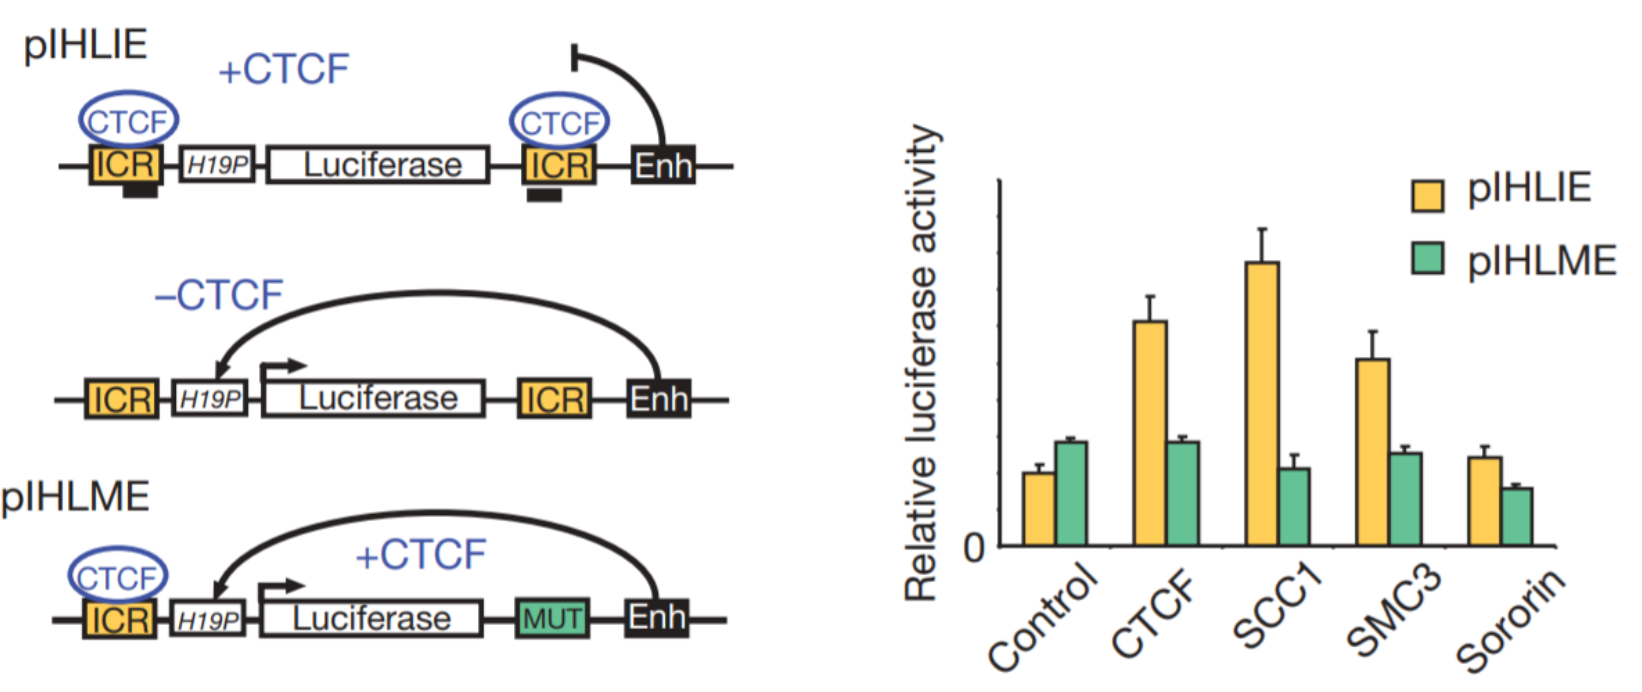
\includegraphics[width=0.8\textwidth]{../_resources/Screenshot_2022-10-14_at_19-50-44.png}
\caption{Wendt et al, Nature, 2008}
\label{fig:rep}
\end{figure}

Cohesin complexes co-localize with CTCF insulator protein and are required for it to block enhancer sequences. (Figure \ref{fig:cohe}). CTCF can slide on DNA and when it reaches an already bound CTCF is stops there $\rightarrow$ functional to repress enhance function (Figure \ref{fig:chrom}).

\begin{figure}[!htb]
   \begin{minipage}{0.48\textwidth}
     \centering
     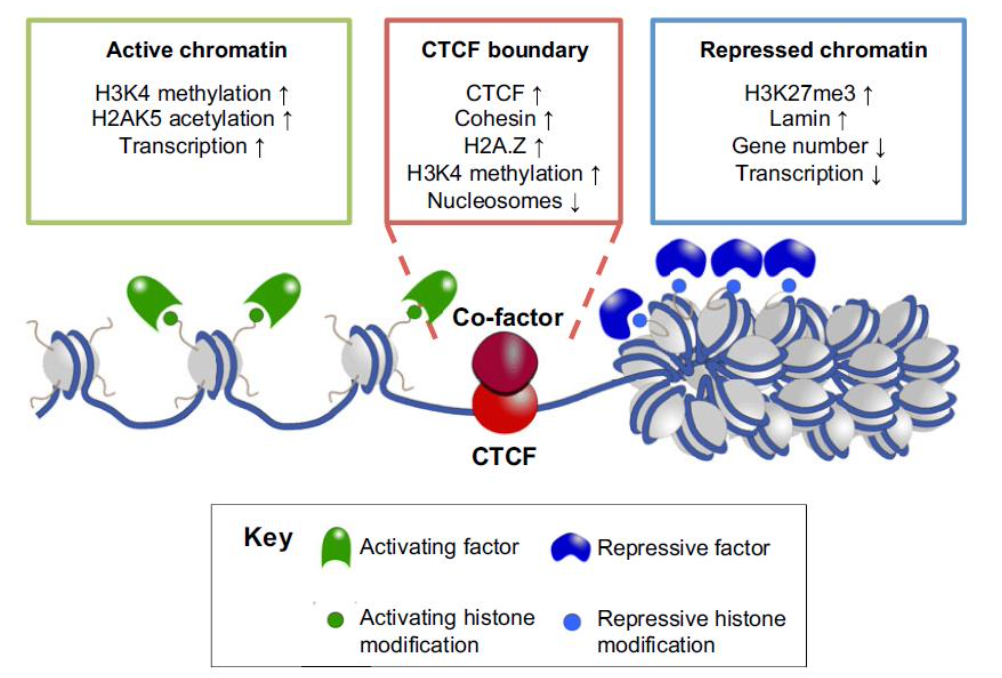
\includegraphics[width=0.6\textwidth]{../_resources/Screenshot_2022-10-14_at_12-11-11.png}
\caption{Herold \emph{et al., Development,} 2012}
\label{fig:chrom}
   \end{minipage}\hfill
   \begin{minipage}{0.48\textwidth}
     \centering
     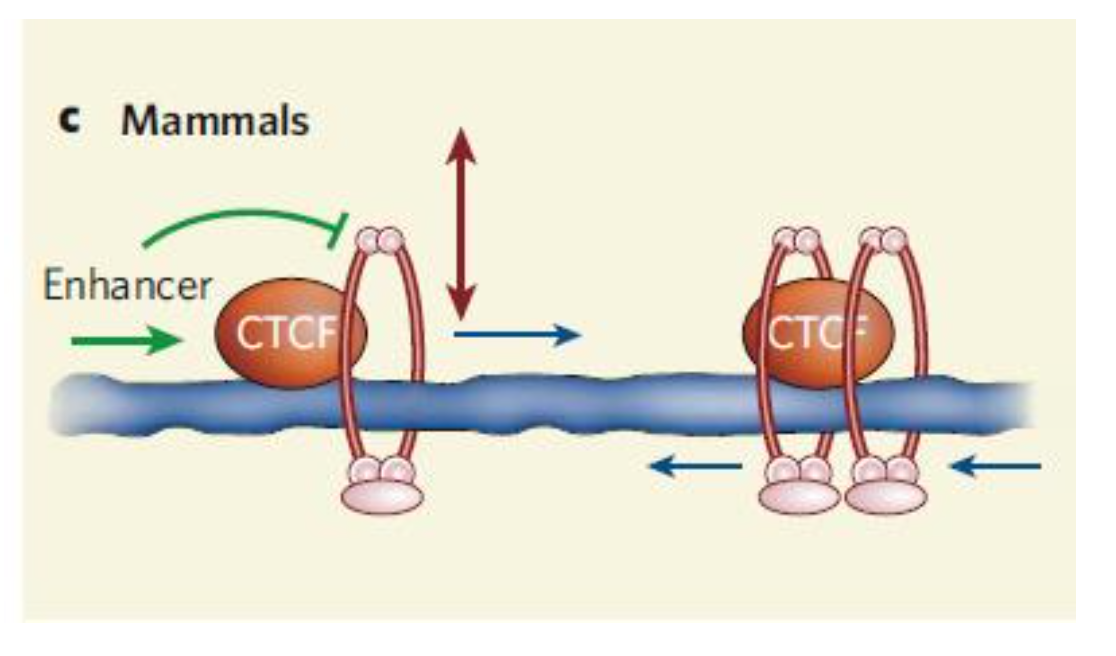
\includegraphics[width=0.5\textwidth]{../_resources/Screenshot_2022-10-14_at_12-10-46.png}
\caption{Parelho et al, Cell, 2008}
\label{fig:cohe}
   \end{minipage}
\end{figure}

\emph{Does cohesin have anything to do with transcription regulation?}
Upon CTCF insulator protein (orange) binding to its DNA consensus sequence, the cohesin ring may tether two DNA double strands (red--blue helices) by encircling them. Thus, \textbf{cohesion-CTCF complexes could shield genes from the effect of enhancer sequences}, regulating gene expression, by impacting genome organization.

\subsection{CTCF and Cohesin in Genome Folding and Transcriptional Gene Regulation}

CTCF binding motifs tend to interact with each other forming a \emph{chromatin loop}. During interphase, DNA is not condensed as in a canonical chromosome, each chromosome forms territories with hierarchical distribution of 3D folding. Different territories can overlap with each other, depending on the extent of histone modificationa. We find compartments, territories and 3D folding of chromatin made by loops. Loops are possibly obtained thanks to the action of cohesins: in \textbf{\emph{loop extrusion}}, a cohesin can slide on DNA for circling 2 ds filaments, until it reaches CTCF is a specific direction. The directionality of CTCF DNA sequences at the loop boundaries indicates the presence of a ``tracking'' mode for DNA loop formation instead of a simple 3D diffusion.

\begin{figure}
\centering
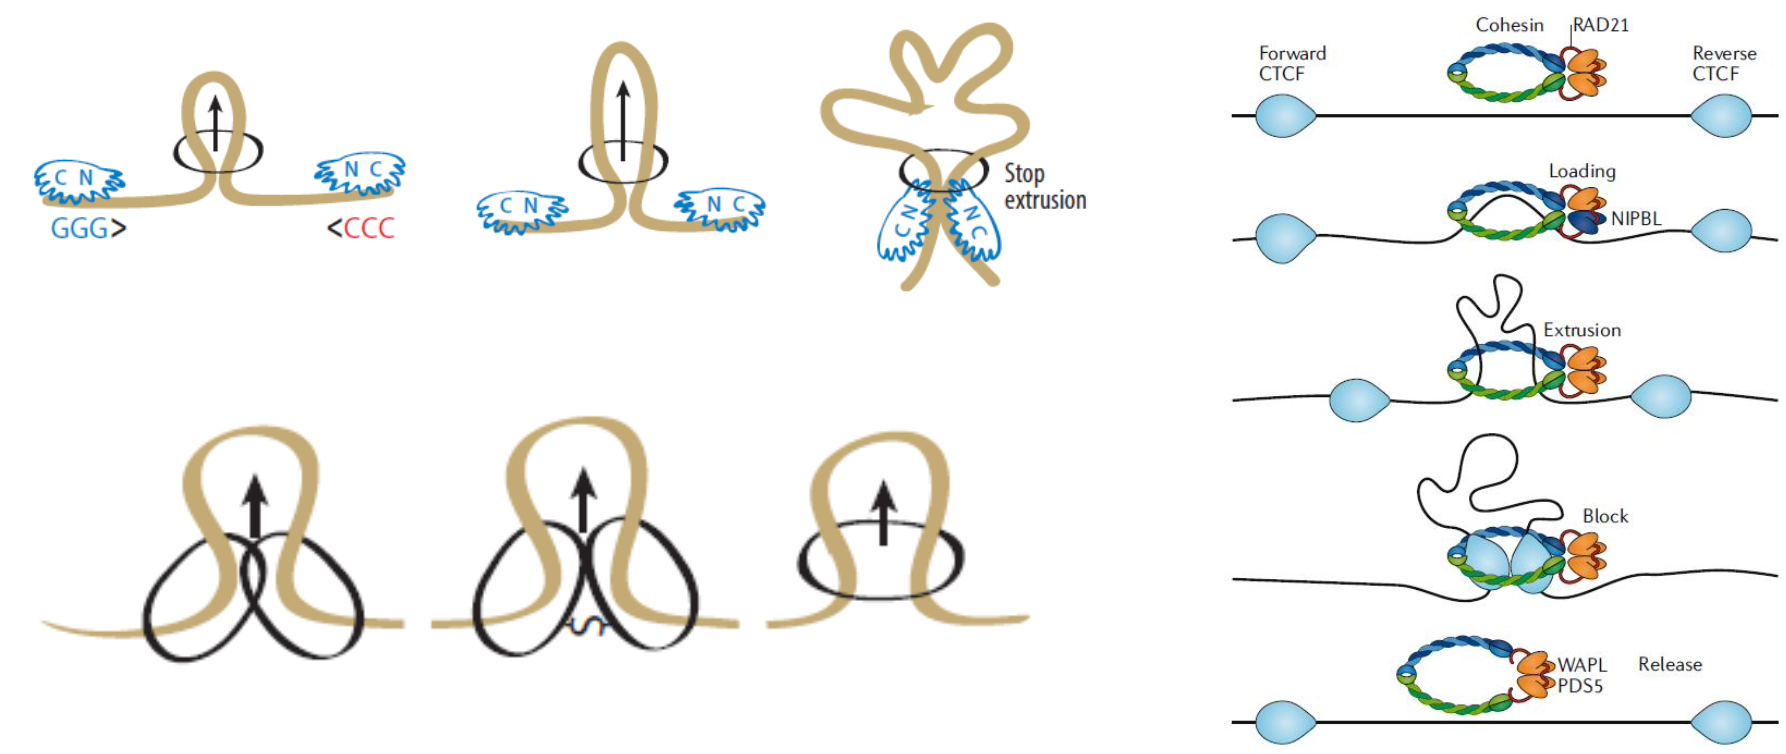
\includegraphics[width=0.6\textwidth]{../_resources/Screenshot_2022-10-14_at_19-52-56.png}
\caption{Merkenschlager and Nora, Ann Rev Gen Hum Genetics, 2016}
\end{figure}

The hierarchical model of chromatin organization impacts gene regulation:
\begin{itemize}
\tightlist
\item
  linear chromosome map
\item
  local 3D folding: local folding brings convergent pairs of CTCF sites in close spatial proximity fostering the contact between the enhancer and the target promoter
\item
  segmentation into TADs: topologically associated domains (TADs) are self associating chromosome segments with high frequency of DNA interaction within them. TADs folding packages enhancers and promoters from the same domain while insulating them from regulatory elements of neighbouring domains.
\item
  compartimentalization of the chromosome territory: euchromatin and heterochromatin compartments. The same compartment can also include DNA from different territories/chromosomes. Compartment A and Compartment B can be subdivided in subcompartments with distinct patterns of histone modifications.
\end{itemize}

Most TADs are constrained within CTCF-cohesin boundaries and may consist of a single or multiple DNA loops called insulated neighborhoods (or loop domains, or sub-TADs).

The sequences that are within a loop are interacting with each other with higher frequency as compared with canonical interaction rates.

The 3D structure of the genome leads to TAD (topologically associated domains), characterized by a high frequency of DNA interaction within them. Compartment A (euchromatin) and B (heterochromatin) can be subdivided in subcompartments with distinct patterns of histone modifications.

Most of the times, TAD consists of one \emph{insulated neighbourhood} (1 loop). We can also find other cohesins inside the same TAD, resulting in \emph{nested} insulated neighbourhoods or \emph{two insulated neighbourhoods}. 90\% of enhancer promoter interactions occur within neighbourhood boundaries in human ESCs and T cells. However, promoters and enhancers do not exclusively interact with each other, as they interact also with other sequences in the same loop.

Chromatin conformation within TADs is highly variable from cell to cell and contacts between DNA loops are dynamic.

\begin{figure}
\centering
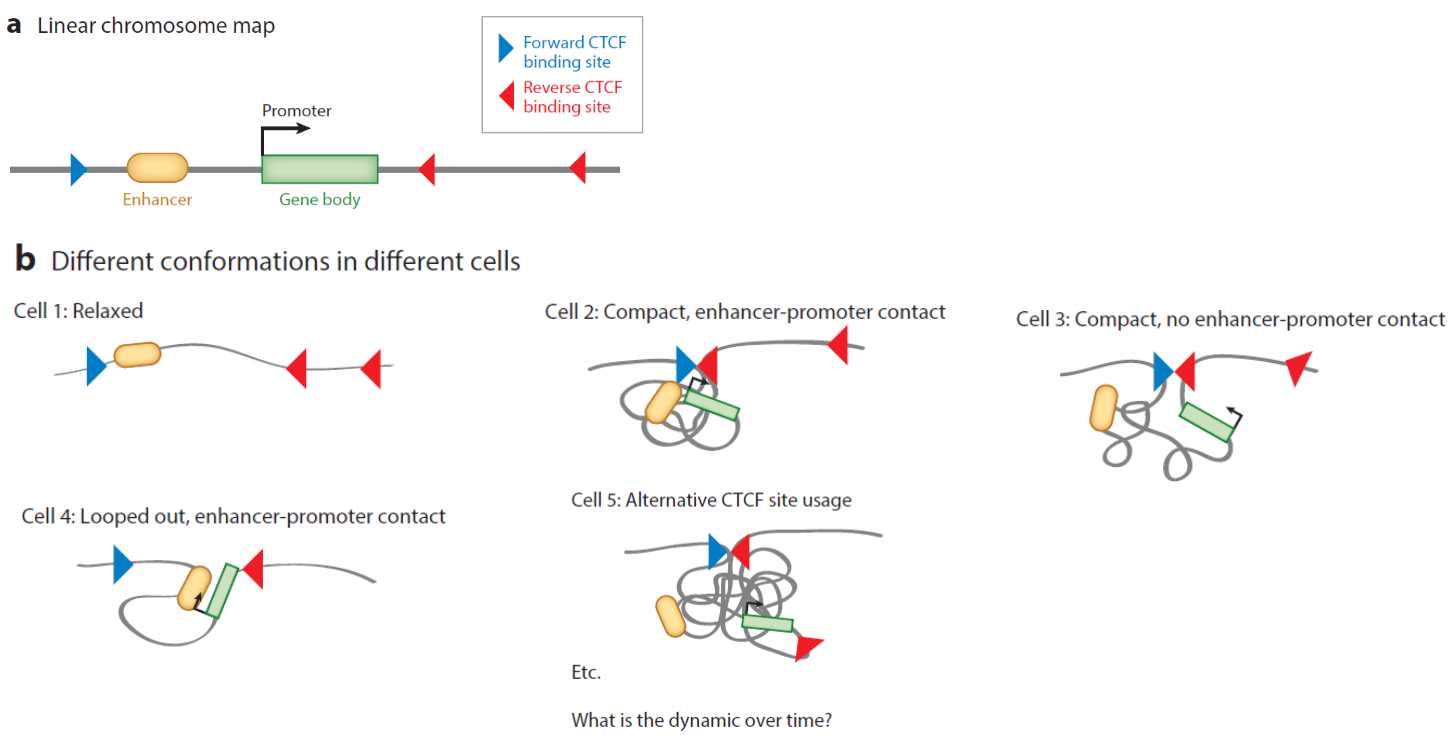
\includegraphics[width=0.8\textwidth]{../_resources/Screenshot_2022-10-19_at_08-48-41.png}
\caption{Merkenschlager and Nora, Ann Rev Gen Hum Genetics, 2016}
\end{figure}

\hypertarget{chromosome-conformation-capture-3c}{%
\section{Chromosome Conformation Capture (3C)}\label{chromosome-conformation-capture-3c}}

This method is used to verify whether distant sequences are interacting in their 3D folding. 3D conformations at the regional, chromosome and whole genome levels can be inferred by calculating the number of ligation junctions between genomic loci.

It is required to have information on all sequences of interest. It is possible to apply inverse PCR: we circularize and amplify from known primers a piece of unknown sequence. In order to test a bigger region, we can use specific primers and verify which sequence is mapped where (computational analysis).

ChIA-PET: which protein is mediating the interaction among two sequences? Use antibody for the protein of interest e.g.~CTCF, pull down cross linked, digest and sequence.

Lastly, in Hi-C approach there is a fill in of the extremities of the restriction sites with biotin and direct sequencing $\rightarrow$ higher throughput.

\hypertarget{hi-c-approach}{%
\section{Hi-C approach}\label{hi-c-approach}}

\begin{enumerate}
\def\labelenumi{\arabic{enumi}.}
\tightlist
\item
  HindIII restriction enzyme
\item
  Fill extremities and mark with biotin
\item
  Ligate (Nhel)
\item
  Purify and shear DNA; pull down biotin
\item
  Sequence using paired-end
\end{enumerate}

A Hi-C map, or \textbf{contact matrix}, is a list of DNA-DNA contacts produced by a Hi-C experiment. Spatial proximity maps of the human genome generated with Hi-C at a resolution of 1 megabase. Each pixel represents all interactions between a 1-Mb locus and another 1-Mb locus.

\begin{figure}
\centering
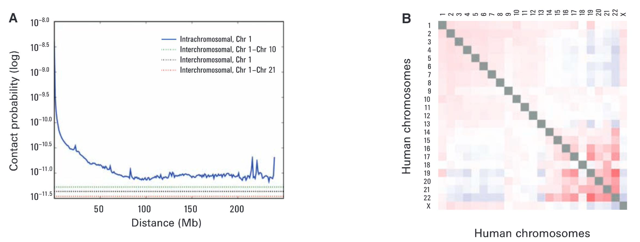
\includegraphics[width=0.7\textwidth]{../_resources/Screenshot_2022-10-25_at_11-47-30.png}
\caption{Lieberma-Aiden \emph{et al., Science} 2009}
\end{figure}

Changing restriction enzyme, a similar pattern is observed. The closer two sequences are in linear form, the higher their contact probability (frequency of interaction).

The probability of contact decreases as a function of genomic distance on chromosome 1. Interchromosomal interactions are depleted relative to intrachromosomal interactions. The level of interchromosomal contact differs for different pairs of chromosomes. This suggests that the chromosomes form defined territories, with an overall frequency of interaction.

Depending on the chromosome, we can find preferential contacts. Example: 20-21-22 region. In low resolution, we observe conserved interaction for synthetic or orthologous sequences.

Each chromosome can be decomposed into two sets of loci (arbitrarily labeled A and B) such that contacts within each set are enriched and contacts between sets are depleted. Regions tend be closer in space if they belong to the same compartment (A versus B).

Bimodal pattern in eigenvector $\rightarrow$ either A or B compartment.

Figure \ref{fig:fish}: 3D-FISH to probe four loci (L1, L2, L3, and L4) on chromosome 14 that alternate between the two compartments (L1 and L3 in compartment A; L2 and L4 in compartment B).

\begin{figure}
\centering
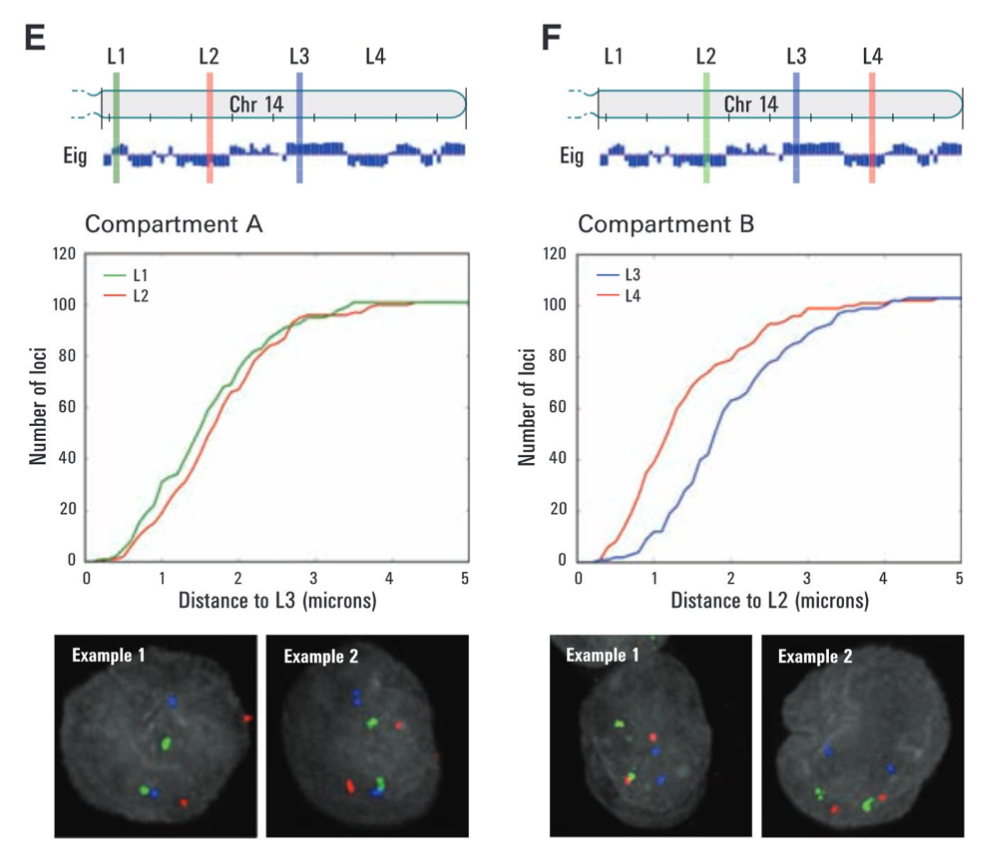
\includegraphics[width=0.5\textwidth]{../_resources/Screenshot_2022-10-19_at_09-06-00.png}
\caption{Lieberma-Aiden \emph{et al., Science} 2009}
\label{fig:fish}
\end{figure}

\begin{itemize}
\tightlist
\item
  Compartment B showed a consistently higher interaction frequency at a given genomic distance than pairs of loci in compartment A, suggesting that it is more densely packed.
\item
  Compartment A correlates strongly with the presence of genes, higher mRNA expression, and accessible chromatin, as measured by DNAse I sensitivity.
\item
  Open and closed chromatin occupies different compartments in the nucleus.
\item
  Such partitioning of the human genome was obtained based on the contact frequency of millions of loci at 1 Mb resolution.
\end{itemize}

\hypertarget{optimization-of-hi-c-approach}{%
\subsection{Optimization of Hi-C approach}\label{optimization-of-hi-c-approach}}

Digestion \emph{in situ}, permeabilize nuclei from cell and without lysing them introduce restriction enzyme cutting 4 nucleotide bases $\rightarrow$ 1kb resolution (Figure \ref{fig:kb}), proximity ligation performed in intact nuclei (reducing the frequency of spurious contacts).

\begin{figure}[!htb]
   \begin{minipage}{0.48\textwidth}
     \centering
     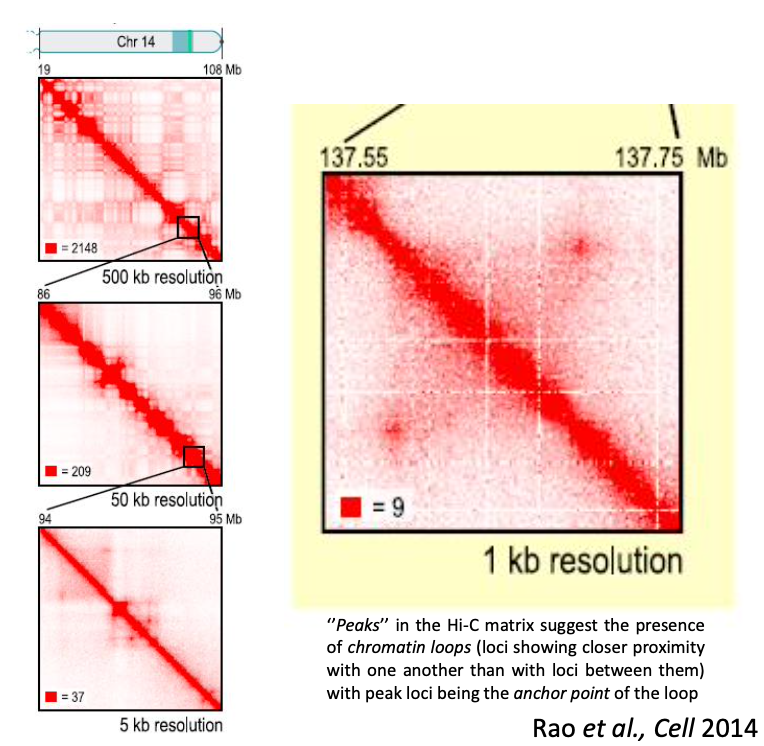
\includegraphics[width=0.7\linewidth]{../_resources/Screenshot_2022-10-19_at_09-10-50.png}
     \caption{}\label{fig:kb}
   \end{minipage}\hfill
   \begin{minipage}{0.48\textwidth}
     \centering
     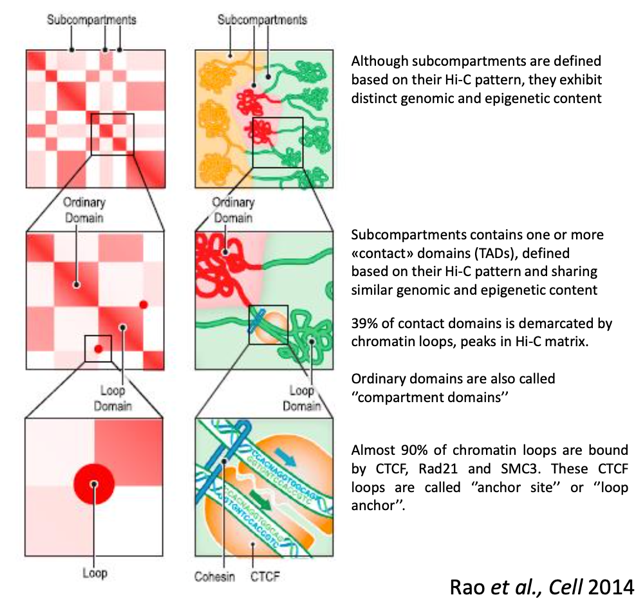
\includegraphics[width=0.7\linewidth]{../_resources/Screenshot_2022-10-19_at_09-11-30.png}
     \caption{}\label{fig:sub}
   \end{minipage}
\end{figure}

We can divide a compartment in 6 subcompartments: A1,A2,B1,B2,B3 and B4. The genomic and epigenetic content is different: different density of active genes, CG richness, epigenetic marks,\ldots{} If we increase the resolution within subcompartments, we find frequently interacting regions, which are called domains:

\begin{itemize}
\tightlist
\item
  \emph{loop domains} (90\% bound by TFs, they are also called ``anchor sites'')
\item
  \emph{ordinary domains or compartment domains}
\end{itemize}

Depending on the resolution, we can define subcomparments or domains TADs (Figure \ref{fig:sub}).

Chromosome compartments are formed by aggregation of multiple domains with similar biochemical or functional properties. In literature some studies indicate `'sub-TADs'' or `'insulated neighborhoods'' to refer to domains identified by high-resolution Hi-C as being smaller than the domains TADs, either ordinary or loop domains.

The frequency of interaction can also be depicted as a linear genomic coordinate. A Hi-C map can be integrated with ChIP-seq and RNA-seq data to assess the complexity of the domains identified by low resolution data.

The identification of TADs is highly dependent on the resolution of the Hi-C data and the scale at which the data are analysed.

\begin{figure}
\centering
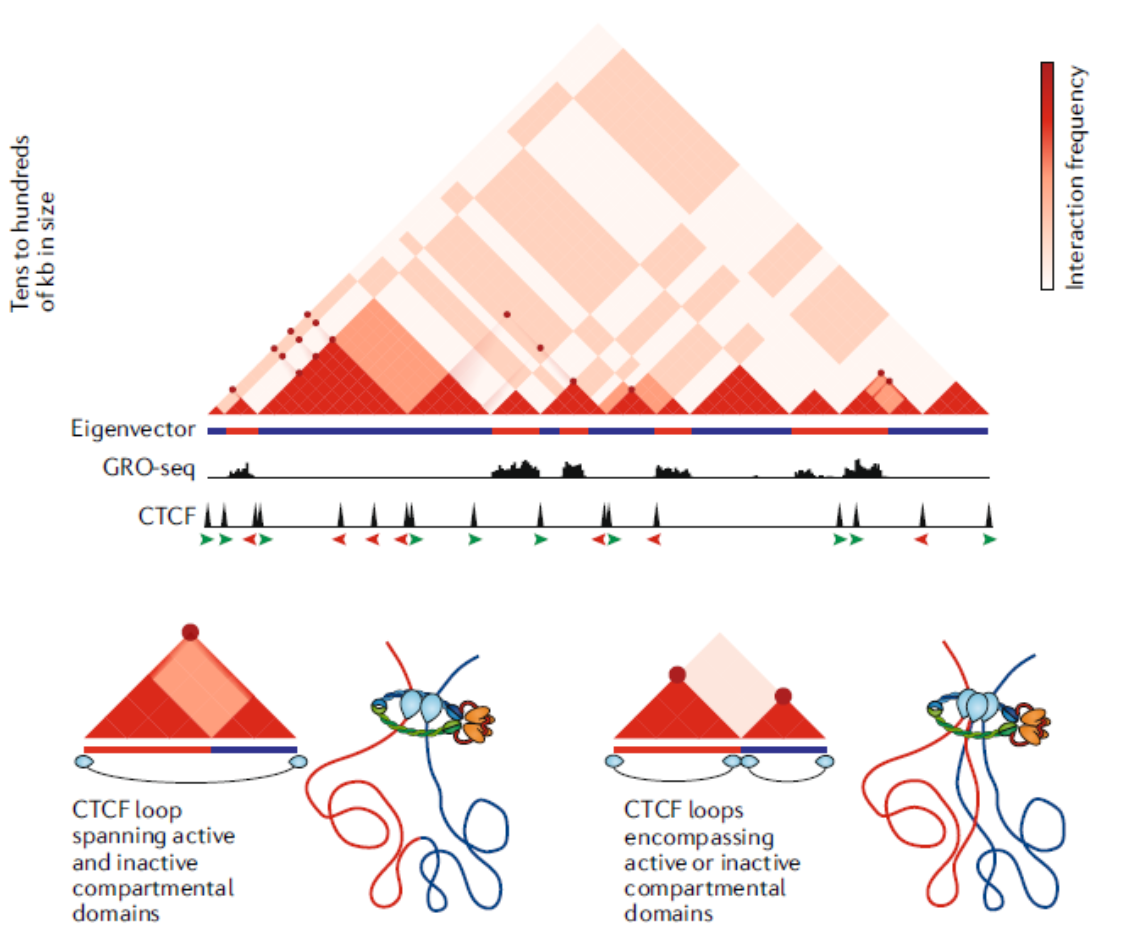
\includegraphics[width=0.5\textwidth]{../_resources/Screenshot_2022-10-19_at_09-20-57.png}
\caption{Rowley and Corces, \emph{Nature Rev Genetics} 2018}
\end{figure}

Some CTCF loops encompass active and inactive domains.

\begin{figure}
\centering
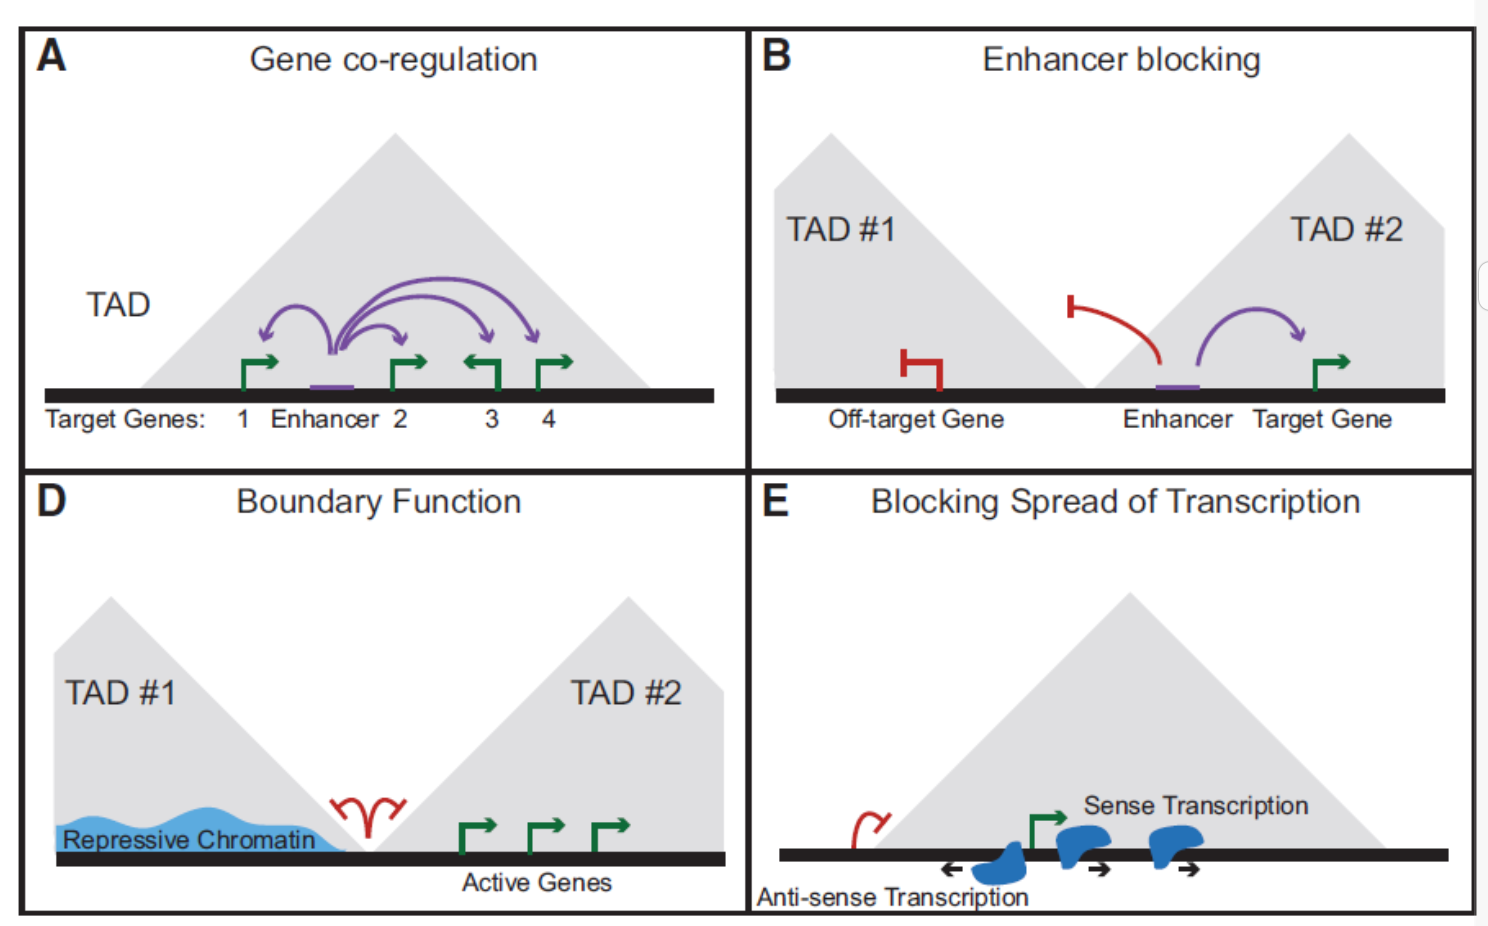
\includegraphics[width=0.5\textwidth]{../_resources/Screenshot_2022-10-19_at_09-21-57.png}
\caption{Dixon \emph{et al., Mol Cell.} 2016}
\end{figure}

Given the high frequency of interaction, we can observe co-regulation favouring. Also, since different TADs do not contain frequently interacting genes, a TAD could feature enhancer blocking. Boundary function: ability of repressing the spreading of heterochromatin. Finally, repressing transcription from one TAD to another.

\textbf{Conclusions:}

\begin{itemize}
\tightlist
\item
  Genomes are partitioned into `contact domains' (ordinary domains or loop domains), or TADs, with median length of 185 kb, that share similar chromatin states and tend to associate with each other forming subcompartments (some people refer TADs to the subcompartments)
\item
  CTCF and the cohesin associate with loop domains and are found at over 86\% of loop anchors.
\item
  The pair of CTCF motifs present at the loop anchors occurs in a convergent orientation in \textgreater90\% of cases
\item
  Loops frequently link promoters and enhancers, correlate with gene activation, and show conservation across cell types and species (up to 75\% are conserved between cell lines, and 50\% between mouse and human orthologous genomic regions)
\end{itemize}

\section{Mediator and cohesin connect gene expression and chromatin architecture}

Enhancers and genes generally interact within the context of the CTCF-CTCF loops which form insulated neighborhoods that constrain interactions between regulatory elements and genes.
This structure helps explain why enhancers generally control only a limited number of genes despite having an ability to function in either orientation and at long distances.

Do enhancers and promoters randomly interact within the same loop domain? Probably not, since single CTCF loops can contain both active and inactive genes.

Enhancer-gene interactions occur in insulated neighborhoods by synergic activity of Mediator and Cohesin, and not CTCF.

Mediator and cohesin physically and functionally connect the enhancers and core promoters of active genes within DNA loop domains in murine embryonic stem cells. When the transcription activators bind mediator, the mediator complex undergoes a conformational change, and this activator-bound form of mediator binds cohesin and its loading factor Nipbl, which all contribute to gene activity and DNA looping. Mediator and cohesin co-occupy different promoters in different cells, thus generating cell-type-specific DNA loops linked to the gene expression program of each cell.

There are different binding sites for cohesin mediator and cohesin CTCF. Distinct overlapping pattern in interaction sites, depletion by shRNA results in a very similar gene expression.

\textbf{Co-IP:}

\begin{enumerate}
\def\labelenumi{\arabic{enumi}.}
\tightlist
\item
  lysate and wash
\item
  add antibody-immobilized agarose resin
\item
  precipitate immune complexes and wash
\item
  analysis by Western blot (nuclear extract vs Co-IP with IgG control)
\end{enumerate}

Adapt Co-IP with ChIP: protein in chromatin complex, instead of extracting RNA de-crosslink and run protein on a gel.

Co-IP results indicate that Cohesin and Mediator interact. Chromosome Comformation Capture (3C) analyses confirmed DNA looping between promoters and enhancers of active genes. Depleting cohesin, frequency of interaction is disrupted, similar as Mediator 12.

Mediator and cohesin physically and functionally connect the enhancers and core
promoters of active genes within DNA loop domains in murine embryonic stem cells

When the transcription activators bind mediator, the mediator complex undergoes a conformational change, and this activator-bound form of mediator binds cohesin and its loading factor Nipbl, which all contribute to gene activity and DNA looping. Mediator and cohesin co-occupy different promoters in different cells, thus generating cell-type-specific DNA loops linked to the gene expression program of each cell.

\hypertarget{promoter-enhancer-communication-occurs-primarily-within-insulated-neighbourhoods}{%
\subsection{Promoter-Enhancer Communication Occurs Primarily within Insulated neighbourhoods}\label{promoter-enhancer-communication-occurs-primarily-within-insulated-neighbourhoods}}

Computational analyses of published CTCF and Smc1 ChIA-PET datasets enabled identification of insulated neighborhoods encompassing 9,407 protein-coding genes of which 3,929 were transcriptionally active in mouse ESCs (Figure \ref{fig:mouse}).

\begin{figure}
\centering
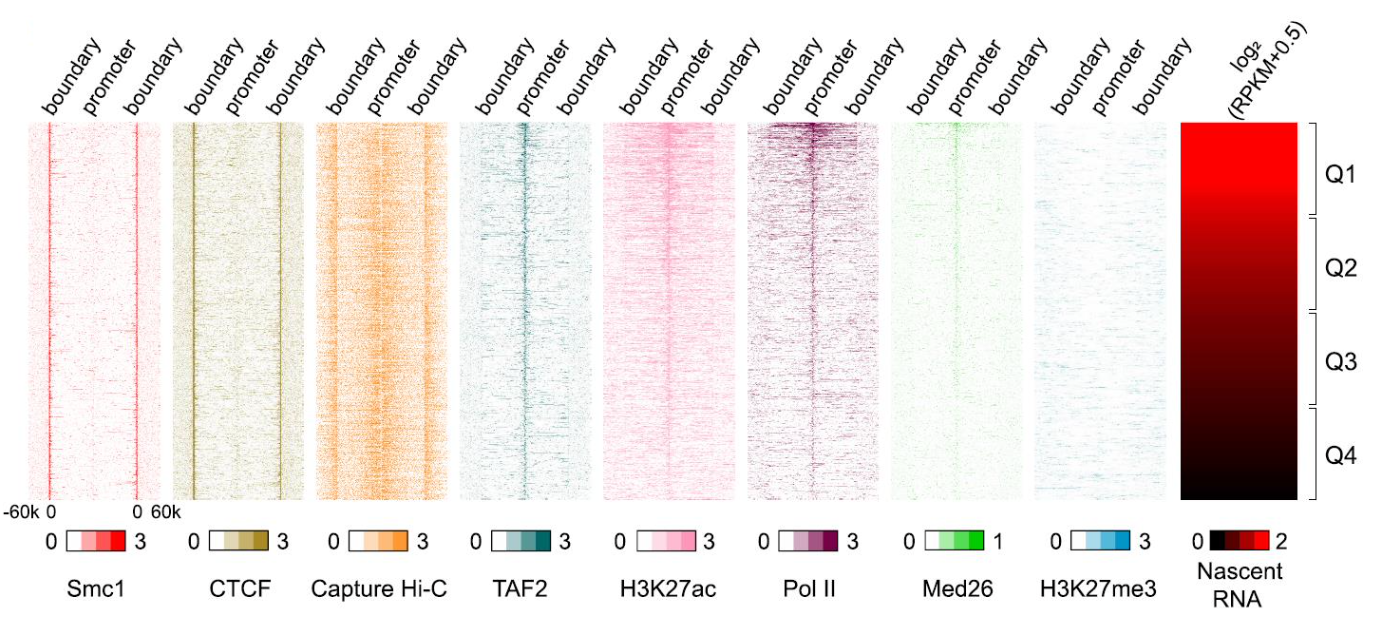
\includegraphics[width=0.5\textwidth]{../_resources/Screenshot_2022-10-19_at_10-01-09.png}
\caption{Sun et al., 2019}
\label{fig:mouse}
\end{figure}

The sites of co-binding of cohesin and CTCF define \emph{DNA loops boundaries}. We can recognize promoters by TAF2 Hac, POL II (not much Med26, repressive).

Enrichment at the boundaries, functional meaning has not yet been defined. Group promoters in quartiles (Q1-Q4) according to efficiency of transcription. The extent of interaction in loops is not necessarily dependent on the frequency of interaction. Capture Hi-C showed that almost 80\% of promoter-interacting loci are constrained within the insulator or at the boundaries; these interactions do not correlate with transcription levels.

Distribution of the indicated proteins binding and promoter Hi-C interactions in insulated neighbourhoods in different RNA expression quartiles.

Promoter sequences form loops predominantly within the insulated neighborhood, in particular with enhancers and boundaries. Are the enhancer function and gene regulation constrained within the same insulated neighborhood? Is it possible to interfere with the function of specific enhancers and test whether it has an effect on genes inside and outside the insulated neighborhood?

Can the Mediator complex be removed from specific genes? They generated a sequence with promoter and TF binding site, anchored to a magnetic bead. Test with Western blot the binding of the protein. The transcription factor estrogen-related receptor b (\textbf{Essrb}) directly interacts with the Mediator complex. Downregulating Essrb would impair Mediator binding to specific enhancers, deregulating expression of distinct target genes.

Indeed, Essrb knock down can be used to deplete Mediator, inactivate enhancers and downregulate target genes.

Now that a system to inactivate enhancers is in place, the authors can test whether enhancer function is constrained within insulated neighborhoods. 222 insulated neighborhoods contained genes downregulated more than 2 folds upon Essrb depletion. Transcription regulation is largely constrained within insulated neighborhoods, and it involves TF-mediator interactions. Is this regulation directly related to promoter- enhancer looping?

\subsection{Depletion of Mediator causes loss of PIC assembly}

Hierarchical structures of chromosomal domains, DNA loops can be clustered, single\ldots{}
Most enhancer-promoter interactions occur during in DNA loops, also called insulated neighborhoods. In the paper, they managed to isolate genes inside the DNA loops.
Hypothesis: in DNA loop are present oncogene, which can be activate by different mechanisms, listed in Figure \ref{fig:proto}.

\begin{figure}
\centering
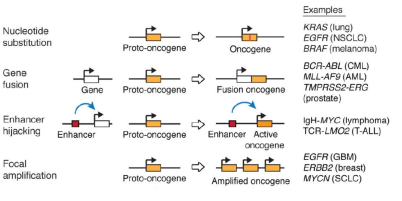
\includegraphics[width=0.5\textwidth]{../_resources/4eb79fba5a169cc3d31f5400dee44c80.png}
\caption{Hnisz et al., Cell, 2016}
\label{fig:proto}
\end{figure}

\emph{Is there a way for DNA loops to promote oncogene transcription?}

In Jurkat cells , 9038 CTCF loops were identified with median length of 270 kb, containing 2-3 genes on average. They crossed adult and embryonic cell lines to discover TADs. Through other analyses they tried to find out presence of loops, enhancer and actively transcripted RNA.

They found out that most cohesin associated enhancer-promoter interactions occurs within CTCF-CTCF loops.

40/55 known oncogenes in the cell line map in insulated neighborhoods. E.g: LMO2 would not usually be transcribed because enclosed in the loop.But with the help of super-enhancers, proto oncogenes like TAL1 can be transcribed.

\textbf{Both active oncogenes and silent proto-oncogenes are located within insulated neighborhoods in Jurkat cells}. 
The main hypothesis states that some insulated neighborhoods function to prevent proto-oncogene activation, then some T-ALL tumor cells may have genetic alterations that perturbs the CTCF bourdaries of neighborhoods containing T-ALL oncogenes.

Example: deletion in promoter of TAL1 -\textgreater{} its transcription is initiated by STIL promoter, which is normally active in T-Cells. TAL1 is normally silenced after fetal stage. Using CRISPr/Cas9 they removed a little piece on the boundary. Disruption of insulated neighborhood boundaries is linked to proto-oncogene activation (Figure \ref{fig:cas}).

The silent state of the TAL1 proto-oncogene is dependent on the integrity of the insulated neighborhood TAL1 encodes a transcription factor that is overexpressed in \textasciitilde50\% of T-ALL cases and is a key oncogenic driver of this cancer (Figure \ref{fig:tal1}).

\begin{figure}[!htb]
   \begin{minipage}{0.48\textwidth}
     \centering
    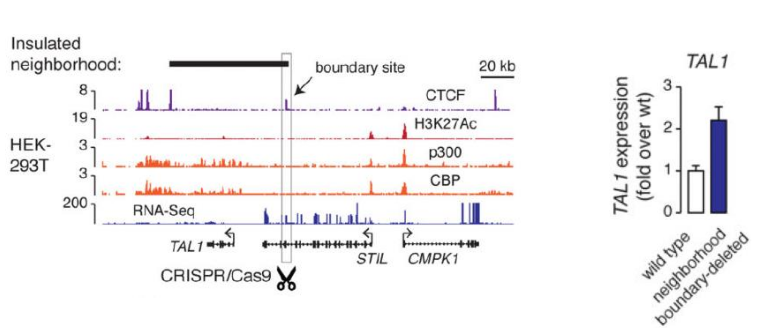
\includegraphics[width=0.5\textwidth]{../_resources/bf32b9679af0fb7fcba57b9f87bb4207.png}
\caption{Hnisz et al., Cell, 2016}
\label{fig:cas}
   \end{minipage}\hfill
   \begin{minipage}{0.48\textwidth}
     \centering
    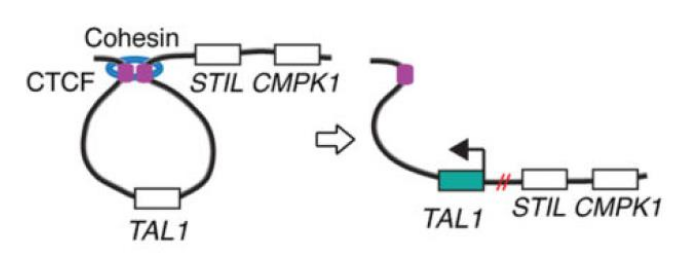
\includegraphics[width=0.5\textwidth]{../_resources/3d83d920d425aa5f76bdbb127596c02b.png}
\caption{Hnisz et al., Cell, 2016}\label{fig:tal1}
   \end{minipage}
\end{figure}

They tried to do the same on another locus, without the mediation of enhancer or promoters. Even in this case,  the disruption of DNA loop allows for the transcription of proto oncogenes.

CTCF in constitutive neighborhoods (present in all cell lines) has a somatic mutation in this cancer, but not the ones in non-boundary CTCF sites (specific to the cell lines). It becomes clear that somatic mutations of insulated neighborhood boundaries occur in the genomes of many different cancers.

\textbf{Main conclusions of the article:}
\begin{itemize}
\item Disruption of insulated neighborhood boundaries, marked by the presence of CTCF and cohesins,
can cause oncogene activation in cancer cells
\item Recurrent perturbations of boundary elements may impact expression of genes with roles in
tumor biology
\end{itemize}

\hypertarget{super-enhancers}{%
\section{Super-enhancers}\label{super-enhancers}}

Super-enhancers regulate genes involved in cell identity: they are bound by tissue-specific TFs and pioneer transcription factors such as OCT4, SOX2, NANOG. They generally activate a self-regulatory circuit: most SE produce promoters, which in turn regulate their own SE and other gene products that they lead.

TAL1 forms transcriptional regulatory networks with other transcription factors in hematopoietic stem cells (Figure \ref{fig:hema}).

\begin{figure}[!htb]
   \begin{minipage}{0.48\textwidth}
     \centering
     \includegraphics[width=0.3\textwidth]{../_resources/99fbd93b812d482263d53c442698a36a.png}
\caption{}
\label{fig:hema}
   \end{minipage}\hfill
   \begin{minipage}{0.48\textwidth}
     \centering
     \includegraphics[width=0.3\textwidth]{../_resources/c099d4a9ad4bba13e7839f48fd831265.png}
\caption{}
\label{fig:talju}
   \end{minipage}
\end{figure}

These circuits underline the tissue-specificity of most cancers. TAL1 requires a SE, a transcriptional re-wiring.
\begin{itemize}
\item The expression of TAL1 is downregulated during normal T-cell development, while GATA3 and RUNX1 are expressed in T cells
\item  Re-expression of TAL1 in T cells dictates a transcriptional circuitry inducing tumorigenesis
\item TAL1, GATA3, RUNX1 and MYB gene loci are associated with super-enhancers in T-ALL cells
\end{itemize}

\hypertarget{how-is-a-se-generated-during-tumorigenesis}{%
\subsection{How is a SE generated during tumorigenesis?}\label{how-is-a-se-generated-during-tumorigenesis}}

Even SNPs can generate super-enhancers! TAL1 SE was not found in T cells, or hematopoietic stem and progenitor cells (HSPCs). 3C experiments identified a looping interaction within the SE (red arrow), not anymore an insulated neighborhood in this particular site (Figure \ref{fig:talju}).

When investigating the reason for this difference, they found out that some nucleotide addition (but not much). Small insertion leads to a TFBS in T-ALL cancer cell lines. Only transcription factors expressed in T-ALL cells are involved in the activation of the mutant enhancer.

BUT a mutation on the promoter of TAL1 is not enough. We need all the transcription circuit of the actors that co-regulate each-other. The Mediator binding pattern stretching for 20kb, overlapping with the H2K27ac mark (seen in previous ChIP), indicates the presence of a super-enhancer. Not observed in HPSCs or T-ALL cells devoid of the mutated TAL1 enhancer site: it is the de novo MYB site to promote TAL1 complex formation and induce TAL1 expression.

ChIP seq revealed the presence of a TAL1 complex, including MYB, at the TAL1 mutated enhancer.
Targeted deletion of the TAL1 enhancer mutation collapses the TAL1 super-enhancer (Figure \ref{fig:deltal}).

This results in a gain of function even in heterozygosity. A SE can be generated by a single transcription factor biding site and can extend to hundred of bases. They are very sensitive to mutations.

Finally, there's mainly two ways to activate proto-oncogenes (Figure \ref{fig:sup}). Both can be triggered by very short deletions/mutations that happen in regulatory regions.

\begin{figure}[!htb]
   \begin{minipage}{0.48\textwidth}
     \centering
    \includegraphics[width=0.7\textwidth]{../_resources/dfb8371fc17e078308c3d5aa247ebcbf.png}
\caption{}
\label{fig:deltal}
   \end{minipage}\hfill
   \begin{minipage}{0.48\textwidth}
     \centering
     \includegraphics[width=0.7\textwidth]{../_resources/8bd5f4820c364c35b02c35eb0e48f464.png}
\caption{}
\label{fig:sup}
   \end{minipage}
\end{figure}

More recent genomic insertions form enhancers that misregulate oncogenes; this hypothesis was tested in different cancer cell lines.

\hypertarget{how-cancer-cells-take-advantage-of-super-enhancers}{%
\subsection{How cancer cells take advantage of super-enhancers}\label{how-cancer-cells-take-advantage-of-super-enhancers}}

In the study \textbf{Identification of focally amplified lineage-specific super-enhancers in human epithelial cancers} scientists interrogated a dataset of 10k tumors and found recurrent focal amplifications. They found 25 peaks which correspond to super-enhancers. They also found that six different cancer cell types had some common recurrent focal amplification in the same spot (Figure \ref{fig:study}).

\begin{figure}
\centering
\includegraphics[width=0.5\textwidth]{../_resources/796c982294bedb0a7994a942aa5ff2a5.png}
\caption{}
\label{fig:study}
\end{figure}

\begin{itemize}
\item UCEC, uterine corpus endometrial carcinoma; 
\item HNSC, head and neck squamous cell carcinoma; 
\item LUAD, lung adenocarcinoma; 
\item CRC, colorectal carcinoma; 
\item LIHC, liver hepatocellular carcinoma; 
\item CESC, cervical squamous cell carcinoma; 
\item ESCA, esophageal carcinoma.
\end{itemize}

\textbf{KLF5} is a putative oncogene that can be upregulated in tumors by super-enhancer amplification.
For the \textbf{MYC} genes, they found data in two different cancer lines. Selectivity of amplification depending on the cell line.
Tumors with amplification of MYC alone or MYC-LASE or MYC-ECSE alone express higher levels of MYC than tumors lacking either amplification (meaning, there's no need for the tumor to evolve a over-expression of MYC).

NFE2L2 and CEBPB transcription factors regulate the e3 enhancer: so to study it, we can downregulate these two factors.

\textbf{Conclusion: MYC regulation changes based on the tumor and tissue type.}
If we are in a cancer setting we can target a super-enhancer and we impact the expression of the target gene. However, there are several onco-genes in a cancer setting.

\hypertarget{the-role-of-myc-in-cancer-cells}{%
\section{The role of MYC in cancer cells}\label{the-role-of-myc-in-cancer-cells}}

In cancer, MYC is always the most amplified gene. MYC is the downstream target of so many pro-proliferation pathways, these cells are not even under selective pressure to activate the pathways.
It has a great impact on cells!

\begin{figure}
\centering
\includegraphics[width=0.5\textwidth]{../_resources/641af477cb65d73954e1ae24aab9a2ed.png}
\caption{Deletion of both Myc and APC from small intenstine cells}
\label{fig:inhi}
\end{figure}

The inhibition of MYC and APC rescues or prevent tumorigenesis. By removing one single target gene we can have drastic results and MYC is capable of driving tumorigenesis on its own (Figure \ref{fig:inhi}).

In most human tumour types, the expression of MYC proteins is deregulated and enhanced relative to the corresponding normal tissue, and high MYC expression often correlates with poor prognosis. \textbf{MYC induces cell proliferation and growth} in the absence of external growth factors. Conversely, inhibition of MYC almost invariably suppresses cell proliferation.
Transgenic mouse studies provided the evidence that deregulated expression of MYC is sufficient to drive tumorigenesis in a number of transgenic mouse tissue.

\hypertarget{key-aspect-of-myc-in-tumorigenesis}{%
\subsection{Key aspects of MYC in tumorigenesis}\label{key-aspect-of-myc-in-tumorigenesis}}

\begin{figure}
\centering
\includegraphics[width=0.5\textwidth]{../_resources/18345a0e70ca9e50883ca61f93ad3405.png}
\caption{Gabai et al., CSHL 2014}
\label{fig:key}
\end{figure}

Cells become addicted to a single oncogene! (and to transcription in general). The key aspects of MYC are recapitulated in Figure \ref{fig:key}.

\hypertarget{myc-transcription-factor-forms-a-heterodimer-with-max}{%
\subsubsection{MYC transcription factor forms a heterodimer with MAX}\label{myc-transcription-factor-forms-a-heterodimer-with-max}}

MYC is quite an unstable protein, even its mRNA has a very short life. It has an one-of-a-kind binding domain, it is a very special protein.

\begin{figure}
\centering
\includegraphics[width=0.5\textwidth]{../_resources/01adbb32a69ee3baec1bf9bddd890f52.png}
\caption{ MYC is a transcription factor forming a heterodimer with MAX}
\label{fig:myc}
\end{figure}

MYC, MAX and MXDI all recognise the same site (Figure \ref{fig:myc}).
MXD and MYC act as antagonists. MXD proteins can recruit histone deacetylases and repress transcription while MYC proteins recruit complexes that promote transcription (not always the case\ldots). MYC stimulates cell growth and proliferation, while MXD inhibits cell growth and proliferation and blocks MYC effects.
MYC-MAX bind to thousands of genes whose identity depends on the cellular transcriptome and the abundance of MYC protein (Figure \ref{fig:maxmyc}).


Studying MYC is very difficult. What we know is that if we do a chIP for MYC we have an extreme range of possible results, result is basically random. For RNA-seq: regulation of genes from MYC is also very subtle, with down-up regualted genes changing like 20\%, but also transcribe for TF that regulate their own site.

\begin{figure}[!htb]
   \begin{minipage}{0.48\textwidth}
     \centering
    \includegraphics[width=0.5\textwidth]{../_resources/017e543a7782177edd93188be60ae382.png}
	\caption{Carroll et al., Front.Med. 2018}
	\label{fig:maxmyc}
   \end{minipage}\hfill
   \begin{minipage}{0.48\textwidth}
     \centering
     \includegraphics[width=0.7\textwidth]{../_resources/e218faf59750ef1a90a9e45629f08973.png}
	\caption{Lourenco et al., Nature Reviews Cancer, 2021}
	\label{fig:regmyc}
   \end{minipage}
\end{figure}

Trunk sustains the outcome of MYC, but the net outcome of MYC interaction and transcription we have epigenetic regulation, pre initiation complex assembly, pause-release behaviour\ldots. 

\begin{figure}
\centering
\includegraphics[width=0.7\textwidth]{../_resources/10a2ad3114504053030a1071443aabd7.png}
\caption{Lourenco et al., Nature Reviews Cancer, 2021}
\label{fig:ppmyc}
\end{figure}

MYC is not a pioneer TF! So important interaction with proteins recruited on the chromatin.
With open chromatin state, we have un-specific transcription. In addition to regulate its own target genes, MYC can `\textbf{amplify}' the transcriptional program already active in a cell, leading to a signature which is cell type-specific. MYC increases the expression of (already poised) thousands of genes (Figure \ref{fig:ppmyc}).

It depends a lot on the level of MYC2: since there are low affinity and high affinity binding sites, the more the MYC the higher the probability of MYC binding the low-affinity regions. Genes can be either down or up regulated.

BUT tumorigenesis is not only about proliferation: we need proteins, membranes,\ldots{} obviously MYC is also involved in anti-apoptosis behaviour, energy metabolism etc.

\begin{figure}
\centering
\includegraphics[width=0.7\textwidth]{../_resources/cdb9692b7dd2ca7bcfae696cd1b1ce36.png}
\caption{Kress et al, NatureRevCancer-2015}
\label{fig:ppmyc}
\end{figure}

\hypertarget{by-which-major-mechanism-or-pathway-myc-proteins-promote-tumorigenesis}{%
\subsection{By which major mechanism or pathway do MYC proteins promote tumorigenesis?}\label{by-which-major-mechanism-or-pathway-myc-proteins-promote-tumorigenesis}}

The final outcome of MYC gene regulation depends on the network of MYC interactions, in particular MYC-MAX
and MAX-MXD and by the transcriptional program of the cells.
MYC is a mild transcriptional modulator, inducing moderate changes in mRNA levels.
It is able to regulate the expression of several other transcription factors and cofactors, including E2F proteins,
Polycomb group repressive complex 2 (PRC2) components, along with microRNAs (miRNAs), thus orchestrating
complex networks of gene regulation.
MYC dependent gene regulation has been shown to be dependent on: cell type, experimental conditions (stress),
levels of MYC.

In conclusion, MYC activation contributes to several hallmarks of cancer:
\begin{enumerate}
\item autonomous proliferation and growth
\item sustained DNA replication
\item increased protein biogenesis
\item global changes in cellular metabolism
\item activation of the angiogenic switch
\item suppression of the response to autocrine and paracrine regulatory programs
\item restraint of host immune responses
\item The transcription rewiring induced by oncogenic Myc levels also renders cancer cells addicted to this particular oncogene
\end{enumerate}

    \graphicspath{{chapters/_resources/}}

\chapter{TCIC}


\hypertarget{transcriptional-control-in-cancer}{%
\section{13- Transcriptional Control in Cancer}\label{transcriptional-control-in-cancer}}

\hypertarget{targeting-transcription-in-cancer}{%
\section{Targeting transcription in cancer}\label{targeting-transcription-in-cancer}}

In order to perform transcription targeting in cancer, we first need to understand which genes are driving tumorigenesis.

\hypertarget{age-related-remodellling-of-oesophageal-epithelia-by-mutated-cancer-drivers}{%
\subsubsection{\texorpdfstring{Age-related remodellling of \textbf{oesophageal epithelia by mutated cancer drivers}}{Age-related remodellling of oesophageal epithelia by mutated cancer drivers}}\label{age-related-remodellling-of-oesophageal-epithelia-by-mutated-cancer-drivers}}

Biopsies from cancer (red) and non-cancer (green) sites from 58 y.o. male with risk for esophagus cancer (smoking and drinking heavily). By looking at the mutational burden, cancer samples has a higher MCF (mutant cell fraction). The normal biopsies showed several mutations too. If we look closer, mutations are hitting driver genes e.g.~NOTCH, TP53. Cancer samples' mutations are overlapping to a good extent and are present at a higher degree. In normal tissues we have \emph{independent mutations,} which suggests that independent clones are present in a normal epithelium.

\begin{figure}
\centering
\includegraphics{../_resources/Screen_Shot_2022-11-04_at_10-50-01.png}
\caption{Yokoyama et al., Nature 2019}
\end{figure}

Yokoyama et al., Nature 2019

Divide patient samples in low and high risk, in normal tissues. The number of mutations per sample increases with risk and over time. By analyzing the mutation, 4 mutational signatures were identified: e.g.~APOBEC is responsible for globulin production, should be restricted to lymphocytes , C→T mutation.

\begin{figure}
\centering
\includegraphics{../_resources/Screen_Shot_2022-11-04_at_10-51-30.png}
\caption{Yokoyama et al., Nature 2019}
\end{figure}

Yokoyama et al., Nature 2019

Normal tissues can accumulate mutations to an extent dependent on lifestyle and age.

Single cell sequencing analysis: the mutation number in colonies from low-risk individuals linearly increases with age with an annual increase of 41.5 mutations per genome per year.

\textbf{\emph{Driver genes}} are mutated in PNE although with different frequencies as compared with
cancer samples and there are substantial differences in the major drivers between PNE and ESCC. Most of the PNE samples from high-risk individuals (62 out of 64, 97\%) contained one or more driver mutations. The positivity of driver mutations was 74\% (69 out of 93) of all samples from low-risk individuals.

\textbf{Spatial distribution and mutational composition of clones within the same biopsy:}

\begin{itemize}
\tightlist
\item
  Young individuals: small number of shared mutations with small MCF. Limited number of driver-mutant clones. During development to early adult life stem cells and their progenies spread giving rise to \textbf{\emph{somatic mosaicism}} more than positive selection.
\item
  Elderly individuals: shared mutations and MCF markedly increase. Driver-mutant clones increase in number and size, a trend which is enhanced with lifestyle ESCC risk. Positive selection may be ongoing.
\end{itemize}

In young individuals we observe a mosaicism of small mutations, while advancing with age we can acquire more mutations which might lead to cell proliferation increase and higher probability of new mutations.

\begin{figure}
\centering
\includegraphics{../_resources/Screen_Shot_2022-11-04_at_10-59-51.png}
\caption{Yokoyama et al., Nature 2019}
\end{figure}

Yokoyama et al., Nature 2019

Some mutations can occur early on in life and they accumulate on specific proliferative pathway they might lead to cancer or not.

80-year-old high-risk man: Divergent clones populating a small epithelial region originated from a single stem cell with a NOTCH1 mutation almost 80 years previously. Positive selection lead to the fixation of 4 driver mutations and subclones formation.
70-year-old high-risk man: Clonal evolution initiated in a stem cell with a TP53 mutation at the age of about 13 years which persisted without evolving to cancer. Meanwhile other driver mutations were acquired.

\textbf{Conclusions}

Mutations inevitably occur in normal cells and accumulate during aging, their frequency depends on lifestyle risks. Such mutations may be positively selected (driver mutations), favoring changes that are beneficial to the individual cells, generating clones. These clones must acquire a number of specific driver mutations to transform generating cancer cells. Normal cells can become cancerous when the `'right'' combination of driver genes has been mutated and/or deregulated. Somatic evolution is not a linear road towards cancer, the clone size, the specific mutations and the tissue context may slow down the tumorigenic process or boost it. Tissues differ substantially in their susceptibility to specific oncogenic events and barriers to tumor formation are tissue specific due to a number of variables, including:

\begin{itemize}
\tightlist
\item
  Tissue-specific oncogenic function of a cancer drivers
\item
  Cell-extrinsic factors such as cell--cell signaling
\item
  The cell of origin and its differentiation status
\end{itemize}

With age, the spreading of mutant clones within tissues may progressively compromise the tissue contributing to aging, cancer and other diseases.

The same pattern was observed in colorectal tissue and especially skin, which has a high burden of somatic mutations.

Standard chemotherapy relies on targeting proliferating cells with alkylating agents. We can also apply precision therapy to certain oncogenes, but this approach should take into account that multiple mutations are present. Over the years, it was observed that if the expression of a target oncogene is repressed, we observe growth inhibition and tumor regression.

Cancer cells can become addicted to the expression of specific oncogenes

Important bias: we are inducing tumorigenesis by inducing overexpression of a single gene, which is not what happens physiologically. However, we know have in clinics drugs targeting different proteins and able to induce tumor regression. One of the first compounds developed was Imatinib, meant to target a kinase fused in CML. Roughly 53 out of 54 patients were cured in phase I clinical trial. All the targets hit by target therapy drugs are enzymes, most of them kinases.

Cancer cells tend to lose cellular functions which are not essential to cell viability or do not increase cellular fitness. This is due to the \emph{genetic drift} determined by the mutational burden, epigenetic modifications, and tumor microenvironment. The silencing of redundant functions and pathways can render cancer cells more susceptible to perturbations. If we hit a particular pathway in a cell, we can impair a function which was previously regulated by multiple pathways → synthetic lethality.

If the domain changes e.g.~accumulation of mutations on oncogene, cancer cells can develop resistance to target therapies. The same happens with new mutations on alternative pathways.

\begin{figure}
\centering
\includegraphics{../_resources/Screen_Shot_2022-11-04_at_11-25-54.png}
\caption{Screen Shot 2022-11-04 at 11.25.54.png}
\end{figure}

 Targeted therapeutics generally lead to resistance

Transcriptional regulators are essential effectors of the transcriptional program imposed by oncogenic drivers, also called transcriptional drivers.

RTK growth factor, frequently hit by mutations in cancer. Resistance can arouse through the persistence of downstream pathway or parallel signaling transduction. This occurs as pathways converge to the same effectors, which are either co-factors regulating transcription or transcription factors. E.g. MYC or beta-catenin, which are also called \emph{transcriptional drivers}.

Example: MYC inhibition eradicates K-RAS (driver oncogene) driven lung cancers in mice.

The consequences of oncogene inactivation for the reversal of tumorigenesis depend on the type of tumor and the genetic context. E.g. if we remove MYC from MYC driven lymphoma, we observe apoptosis of lymphoma cells. In hepatocellular carcinoma, the re-expression of MYC leads to restoring cancer. Cancer cells can escape dependence on oncogenes by acquiring other genetic events.

\hypertarget{key-points}{%
\subsubsection{Key points}\label{key-points}}

Cancer is caused primarily by genetic mutations and is initiated and maintained by recurrent driver mutations. Cancer cells genome undergoes a constant genetic drift. Transcription deregulation is a hallmark of cancer, as cancer cells inevitably undergo transcription rewiring. Dysregulated transcriptional programs fuel tumorigenesis. Cancers can remain addicted to the oncogenes that have driven tumorigenesis and/or to the transcriptional drivers (definitive cancer drivers). Dysregulated transcription also creates transcriptional dependencies which are not typically identified by cancer genome sequencing. \textbf{Transcriptional addiction} in cancer can be harnessed for therapeutic intervention.

Resistance to targeted therapy can occur by activating \emph{alternative signaling molecules} and pathways converging on the same transcriptional regulators or by \emph{acquiring mutations} on the targeted gene.

Transcriptional regulators act as effectors of the oncogenic drivers. Cancer cells can become as `'addicted'' to these effectors as they are to the oncogenic drivers.

The complexity of TFs networks renders resistance mechanisms difficult to be developed.

Transcription factors interact in complex networks, also involving other transcription regulators. It is unlikely that any TF, or non-TFs transcriptional regulators such as CBP-p300, BRD4, can be completely replaced by another. It is more difficult to bypass this particular targeting.

\begin{figure}
\centering
\includegraphics{../_resources/Screen_Shot_2022-11-04_at_11-51-12.png}
\caption{Gonda and Ramsay, \emph{Nature Review Mol Cell Biology}, 2015}
\end{figure}

Gonda and Ramsay, \emph{Nature Review Mol Cell Biology}, 2015

Targeting transcription regulators will have a lower likelihood of emergence of resistance than targeting intracellular signaling pathways, also because multiple pathways can converge on the same transcription regulator. Inhibiting a specific transcriptional program may impact more than one oncogenic signal. The main issue is to identify transcriptional drivers, which might not be affected by mutations; it is required to perform wet lab experiments. Furthermore, target mutations can still emerge as resistance mechanism.

\hypertarget{target-transcription-in-cancer}{%
\subsection{Target transcription in cancer}\label{target-transcription-in-cancer}}

There exist numerous ways to target transcription in cancer:

\begin{itemize}
\tightlist
\item
  interaction with co-factor
\item
  interaction with ligand → most effective mechanism, clinical trials
\item
  PTM
\item
  TF-TF interaction
\item
  impairing recruitment to responsive elements
\end{itemize}

The mechanism of action can be PROTAC or monomeric degradation: they bind their own target and promote degradation. The \textbf{monomeric degrader} can alter 3D structure to make accessible to proteosomal degradation. \textbf{PROTAC} has a domain for E3 ligase, which leads to the recruitment of protease. In principle these molecules can interact with any region of the protein e.g.~epitope, AA sequence (not necessarily domain). Once the protein is degraded, the molecule is still around and can be recycled to degrade other proteins (1:1 stoichiometry is not required).

\begin{figure}
\centering
\includegraphics{../_resources/Screen_Shot_2022-11-04_at_11-55-34.png}
\caption{Bywater \emph{et al., Nature Review Cancer-} 2013}
\end{figure}

Bywater \emph{et al., Nature Review Cancer-} 2013

The Mediator and other complexes are controlled by kinases, so we can foster their inhibition.

THZ1 interacts with the ATP binding pocket of CDK-7, covalent bond with Cys321. In the study the THZ1-R,R was used as a control, as it should not achieve Cys binding.

By pulling down THZ1, we can visualize CDK7 activity: by increasing the amount of THZ1, the competition with bio-THZ1 is overcome and CDK7 expression is inhibited. RNAPII phosphorylation is impaired in vitro with high amounts of THZ1. If the experiment is performed with mutated C312S, phosphorylation of Pol II is not inhibited anymore.

Washout experiment: treat compound, wash and let cells grow without the compound. In this case CDK7 inhibition persists, since it is irreversible thanks to covalent binding.

THZ1 treatment shows broad antiproliferative activity in cancer cell lines by modulation of transcription.

High throughput screening of cell lines in micro plates to test cell proliferation shows that T-ALL cells are particularly sensitive to small perturbations in transcription and CDK7 kinase function. Instead BJ fibroblasts and RPE-1 were not affected.

Bioluminescent xenografted mouse model confirmed efficacy of THZ1 in blocking tumorigenesis of the human T-ALL cell-line KOPTK1. No toxicity of the compound was observed in mice. High doses of THZ1 were required to impair proliferation of non transformed cells.

\emph{Why do cancer cells and in particular T-ALL cells are more sensitive to CDK7 inhibition than non cancer cells?} By applying 250 nM of THZ1 we observe the reduction of transcription of all genes. If we lower the concentration at 50 nM, only a subset of genes will be impacted e.g.~TAL1, GATA3, RUNx1 → super enhancer region, these factors autoregulate their own gene expression while simultaneously regulating many other genes.

 RUNX1 forms a core regulatory circuitry with TAL1 and GATA3 transcription factors that have prominent roles in leukaemia biology

\textbf{Takehome message:}

Targeting transcription is a promising anticancer approach which can be achieved by CDK7 inhibition. Transcription rewiring of cancer cells can be triggered by acquisition of super-enhancers driving oncogene expression and tumorigenesis. Super-enhancer driven oncogenes lead to transcription addiction generating transcriptional dependencies which can be used for therapeutic intervention. Cancer cells require continuous active transcription which renders them more sensitive to transcription targeting therapeutics. In particular oncogenic drivers like MYC and RUNX1 have short mRNA and protein half-lives and depends on continuous transcription. Genomic sequences may not suffice to identify driver oncogenes and cancer vulnerabilities.

\hypertarget{transcriptional-control-in-cancer}{%
\section{15- Transcriptional Control in Cancer}\label{transcriptional-control-in-cancer}}

\hypertarget{brd4}{%
\section{BRD4}\label{brd4}}

BRD4 is a member of the Bromodomain and Extraterminal (BET) family along
with BRD2, BRD3 and BRDT. It is a histone acetyltransferase that evicts nucleosomes from chromatin. In particular, BET inhibitors impair super-enhancer driven oncogene expression.
****

\begin{figure}
\centering
\includegraphics{../_resources/Screen_Shot_2022-11-13_at_19-35-28.png}
\caption{Screen Shot 2022-11-13 at 19-35-28.png}
\end{figure}

\hypertarget{selective-inhibition-of-tumor-oncogenes-by-disruption-of-super-enhancers}{%
\subsubsection{Selective inhibition of Tumor Oncogenes by Disruption of Super-Enhancers}\label{selective-inhibition-of-tumor-oncogenes-by-disruption-of-super-enhancers}}

Super-enhancers associated genes were expressed at higher levels than enhancer-driven genes and specifically in mieloma cell line. The majority of super enhancer associated genes were previously shown to be involved in mieloma tumorigenesis e.g.~MYC, CCND2. Treatment of MM1 cells with Brd4 inhibitor JQ1 resulted in reduced levels of BRD4 at enhancers and promoters.

JQ1 treatment lead to more pronounced reduction of BRD4 enrichment at super- enhancers showing almost complete loss of BRD4; in particular, super-enhancers are more sensitive to BRD4 inhibition than regular enhancers. MYC is among the most rapidly depleted genes upon BRD4 inhibition.

Genes associated with super-enhancers showed greater decrease in RNApol II at gene body than the ones associated with enhancers.

\begin{itemize}
\tightlist
\item
  Cancer cells can acquire super-enhancers (SE) as mechanism to drive oncogene expression
\item
  SE are characterized by disproportionately high levels of BRD4 and Mediator, interacting with each other and with multiple cofactors
\item
  SE are highly reliant on cooperatively interacting factors and lose activity more rapidly (than enhancers) when the levels of SE-bound factors are reduced
\item
  BRD4 inhibition leads to preferential disruption of SE driving critical oncogenes in cancer cells
\end{itemize}

The molecular details underlining cancer cells addiction to BRD4 are being unveiled.

\hypertarget{yaptaz}{%
\section{YAP/TAZ}\label{yaptaz}}

The transcriptional coactivators YAP (Yes-associated protein)/ TAZ (transcriptional coactivator with PDZ-binding motif) and their interactors.

\begin{figure}
\centering
\includegraphics{../_resources/Screen_Shot_2022-11-13_at_19-40-17.png}
\caption{Screen Shot 2022-11-13 at 19-40-17.png}
\end{figure}

The \textbf{HIPPO signalling} regulates YAP/TAZ and epithelial architecture and cell polarity are inhibitors of YAP/TAZ → EMT triggers inactivation of the Hippo cascade and YAP/TAZ activation.

\begin{figure}
\centering
\includegraphics{../_resources/Screen_Shot_2022-11-13_at_19-41-35.png}
\caption{Screen Shot 2022-11-13 at 19-41-35.png}
\end{figure}

Mechanical signals are ubiquitous, targeting every cell in every tissue. Mechanotransduction converge on YAP/TAZ in multiple cellular contexts.

YAP and TAZ are nuclear effectors of mechanical signals exerted by ECM and cell shape:

\begin{figure}
\centering
\includegraphics{../_resources/Screen_Shot_2022-11-13_at_19-43-07.png}
\caption{Dupont et al., Nature 2011}
\end{figure}

Dupont et al., Nature 2011

The process of tumorigenesis is accompanied by collagen crosslinking, ECM stiffening, and increased focal adhesions. YAP/TAZ activity is controlled by cell shape and polarity through the cytoscheletal structure which also senses the topology and the rigidity of the extracellular matrix.

Cells probe the physical features of the microenvironment through integrins and adesive proteins responding to extracellular forces by adjusting their tensional state through the cytoscheleton activity. Physical and mechanical cues transmitted by the extracellular environment (i.e.: stiffness of the ECM) reach the nucleus at least in part by YAP/TAZ activation.

YAP/TAZ interact with the TEAD transcription factors to regulate gene expression.

\hypertarget{tead}{%
\section{TEAD}\label{tead}}

\begin{figure}
\centering
\includegraphics{../_resources/Screen_Shot_2022-11-13_at_19-48-01.png}
\caption{Screen Shot 2022-11-13 at 19-48-01.png}
\end{figure}

TEAD is regulated by Hippo, Wnt, TGF-beta and EGFR pathway and is responsible for controlling drug resistance, metastasis, EMT and cancer stem cells. TEAD-driven transcriptional targets include well-established genes that are involved in cell growth, proliferation, and tissue homeostasis. YAP/TAZ drive several key attributes of cancer cells.

\hypertarget{yaptaztead}{%
\subsection{YAP/TAZ/TEAD}\label{yaptaztead}}

Mapping YAP/TAZ/TEAD associations with chromatin in breast cancer cells reveals that these regulators associate with active enhancers. Hi-C analyses predict about 3000 genes regulated by YAP/TAZ/TEAD. 3C analyses confirmed YAP/TAZ/TEAD binding to MYC and TOP2A enhancers.

YAP/TAZ are required for activation of MYC and TOP2A enhancers.

YAP/TAZ-depleted cells stop proliferating and accumulate in G1.

TEAD depletion phenocopies YAP/TAZ depletion → TEAD is determinant for YAP/TAZ induced proliferation. Most YAP/TAZ motifs contained both TEAD and AP-1 motif.

Requirement of AP-1 for YAP/TAZ/TEAD induced transcription program tumorigenesis.

YAP/TAZ interact with the TEAD transcription factors to regulate gene expression. AP-1 enhances YAP/TAZ/TEAD transcription program and tumorigenesis

BRD4 inhibition impacts the YAP/TAZ transcriptional program in the MDA-MB-231 breast cancer cell line → \textbf{Brd4 is required for YAP/TAZ-mediated transcriptional regulation}. In addition YAP/TAZ are required for BRD4 recruitment to chromatin.

Conclusions:

\begin{itemize}
\tightlist
\item
  YAP/TAZ and BRD4 associate physically and functionally in breast cancer cell lines
\item
  YAP/TAZ-BRD4 complex confers a transcriptional advantage to a broad YAP/TAZ targets the expression of these genes can be targeted by BET inhibitors
\item
  Super-enhancers consist of YAP/TAZ-occupied enhancers showing strong enrichment of BRD4, high expression levels of regulated genes and higher sensitivity to BET inhibitors than average
\item
  Oncogenic effect of BRD4 in association to YAP/TAZ offers a new perspective:
  to stratify patients which are more likely to benefit from BET inhibitors, alone or in combination with other drugs
\item
  Development of new therapeutic approach around YAP/TAZ-BET interaction surfaces
\end{itemize}

→ YAP/TAZ represent ideal candidates to mediate cancer-specific transcriptional addictions
and potential drug targets
****

\hypertarget{transcriptional-control-in-cancer}{%
\section{17- Transcriptional Control in Cancer}\label{transcriptional-control-in-cancer}}

Recap

{[}\ldots{]} copy from slides

The inhibition of BRD4 could represent an important mechanism to target.

If we analyze tumorigenic mechanisms in vivo and in vitro we will observe different results: processes dictated by the microenvironment will significantly impact on the tumorigenic potential of cancer cells.

Binary pan-cancer: YAP/TAZ are upregulated oncogenes. Cancers that do not express YAP/TAZ can silence its expression, as it will lead to cell death and differentiation. The effect of YAP/TAZ all depends on the transcriptional program. It is possible to impair YAP/TAZ through targeted therapies e.g.~Tyr kinase inhibitors or Ser/Thr kinase inhibitors; however we must be careful, as resistance can arise. When the transcriptional program is inhibited, tumor suppression is observed. In the case of YAPoff cancers we observe the expression of MYC, which could be targeted. If we manage to re-express YAP/TAZ, they will bind to TEAD and bHLH activating genes promoting adhesion and cell differentiation, always resulting in tumor suppression.

\begin{figure}
\centering
\includegraphics{../_resources/Screen_Shot_2022-11-18_at_11-11-12.png}
\caption{Screen Shot 2022-11-18 at 11-11-12.png}
\end{figure}

\hypertarget{nuclear-receptors}{%
\section{Nuclear receptors}\label{nuclear-receptors}}

Nuclear receptors are transcription factors which mediate transcription regulation upon receptor-specific ligand binding. Usually NR are found bound to DNA in the nucleus or to other proteins in the cytoplasm. In most of the cases they are hetero or homodimers. Nuclear receptors share a common architecture - very conserved modular structure composed by 2 transactivator domains, DNA binding domain and C terminus ligand binding domain (11 helices forming a pocket, 12th helix outside acting as a pocket closure) - and functional behavior. NR are involved in many processes and in different forms of cancer e.g.~estrogen receptor alpha ((ER$\alpha$)).

ER$\alpha$ is associated with proliferation and development and cells for the formation of tissues and organs in women. ER$\beta$ has the opposite function, it is repressing proliferation. ER$\alpha$ is expressed in mammary glands and uterus., ER$\beta$ colon or immune system cells. It is still unclear how the two behave so differently, probably specific TF interaction.

\hypertarget{estrogen-receptor-alpha}{%
\subsection{\texorpdfstring{Estrogen receptor \(\alpha\)}{Estrogen receptor \textbackslash alpha}}\label{estrogen-receptor-alpha}}

Estradiol induces dimerization of ER and binding of the dimer to ER response elements (EREs). ER$\alpha$ binds to HSPs and when estradiol is met we observe the conformational change leading to ERE binding. For achieving a complete activation of the NR, PTMs are required e.g.~Cdk7 targets S118 for phosphorylation.

The main antagonists of ER are known as \textbf{SERM} and \textbf{SERD}. The first target therapy for ER, \emph{Tamoxifen}, was developed in the late 60s. Tamoxifen belongs to SERM, modulator interacting with ER, impairing the ability to interact with the binding site. Once ER binds it cannot recruit co-regulators, its transcriptional action is shut down. Short term Tamoxifen treatment does not show high survival rates, but longer times expose patients to side effects e.g.~acts as agonist for ER in endometrial cells. Other drugs from SERM family act similarly e.g.~Raloxifene and Bazedoxifene. In addition to SERM, we have ER degraders from SERD family → through degradation PTMs e.g.~sumoylation. Fulvestrant is a steroid derivative molecule (quite different from Tamoxifen), not water soluble so needs to be injected in muscles.

\begin{figure}
\centering
\includegraphics[width=0.5\textwidth]{../_resources/Screen_Shot_2022-11-18_at_11-06-54.png}
\caption{Screen Shot 2022-11-18 at 11-06-54.png}
\end{figure}

The two major strategies for therapeutic targeting of hormonal signaling in breast cancer are \emph{direct antagonism} of the ER and \emph{estrogen deprivation}. Aromatase inhibitors can avoid estradiol production in order to deactivate ER activation.

\begin{figure}
\centering
\includegraphics[width=0.5\textwidth]{../_resources/Screen_Shot_2022-11-18_at_11-14-09.png}
\caption{Screen Shot 2022-11-18 at 11-14-09.png}
\end{figure}


\subsection{ER$\alpha$) in breast cancer}

\begin{itemize}
\tightlist
\item
  Nearly 75\% of breast cancers are driven by ER$\alpha$-mediated transcriptional activity
\item
  Estrogen deprivation and direct antagonism of ER represent the two major strategies for therapeutic targeting of ER+ breast cancers
\item
  More than 20\% of patients develop resistance to anti-estrogens and relapse with metastatic disease
\end{itemize}

\hypertarget{mechanisms-provoking-breast-cancer-drug-resistance}{%
\subsubsection{Mechanisms provoking breast cancer drug resistance}\label{mechanisms-provoking-breast-cancer-drug-resistance}}

Clinical sequencing of 11 metastatic ER-positive breast cancer cases before and after therapy showed that \textbf{ESR1 mutations} were not present at an earlier stage, indicating that they were acquired after endocrine therapy. Tumors had survived estrogen targeting or deprivation treatments by acquiring ESR1 mutations.

ESR1 alterations are focused on H12 of the LBD. Analyses of 390 ER-positive breast cancers (primary tumors, before hormonal treatment) from the TCGA revealed no LBD-disrupting mutations of ESR1.

ESR1 with acquired mutations encode constitutively active proteins functioning in the absence of ligand → resistance mechanism. The mutated ESR1 variants are active in the absence of estrogen and continue to be responsive to direct ER antagonists. These mutations might not have been arisen under selective pressure of anti-estrogen treatment but rather in the context of an estrogen deprivation setting, such as treatment with aromatase inhibitors and/or oophorectomy. 67.4\% of the ESR1-mutant metastatic patients had prior exposure to an aromatase inhibitors.

The presence of a somatic mutation in the LBD of ESR1 does not necessarily imply constitutive activity. The most frequent mutation is D538G. Most mutations were activating ER in the absence of estradiol. ER mutants show increased S118 and S167 steady state phosphorylation.

Fulvestrant (ICI) was able to inhibit the activity of all of the mutants which however showed significant differences in sensitivity to the drug. Y537S mutants displayed 70-fold higher IC99 than WT ER, while E380Q and S463P showed 2-fold higher IC99. Fulvestrant fully inhibited the growth of the WT-, E380Q-, and S463P expressing tumors while nearly completely inhibiting the growth of D538G tumors. The Y537S-expressing tumors, however, continued to grow in the presence of fulvestrant, albeit more slowly than in untreated controls, AZD9496 was able to completely inhibit their growth.

These findings are consistent with results from a subsequent clinical trial identifying the ER$\alpha$ Y537S as an acquired mutation promoting resistance to fulvestrant treatment.
Patients previously progressing on endocrine therapy were enrolled for either palbociclib plus fulvestrant or placebo plus fulvestrant treatment, demonstrating an improvement in median PFS from 4.6 to 11.2 months with the addition of palbociclib to fulvestrant. Acquisition of new PIK3CA and ESR1 mutations, in particular the ESR1 Y537S mutation, in both treatment arms implicates these changes in the development of parallel mechanisms of resistance and suggest potential new avenues for treatment.

\hypertarget{summary}{%
\subsubsection{Summary}\label{summary}}

\begin{itemize}
\tightlist
\item
  \emph{ESR1 gene mutations} are found in about \textbf{14\% of breast cancer metastasis}
\item
  Most ER mutations promote an activated conformation in the absence of ligand which remains
  permissive for ligand binding, thus a direct antagonism may be a strategy for these mutants
\item
  Mutations behave differently in terms of ER activity and sensitivity to drugs
\item
  Mutated-ER proteins can be inhibited by \emph{fulvestrant} and \emph{AZD9496,} Y537Y mutation is more resistant to fulvestrant
\item
  Mutation of Y537 site to cysteine (C), aspartic acid (D), and asparagine (N) caused receptor
  activation, but to a lesser degree than did the S mutant. Hence, the level of ER activation depends on both the site of mutation and the nature of the mutant residue
\item
  Tumor genotyping of \emph{ESR1} mutant breast cancers also revealed recurrent alterations in the
  PI3K/AKT pathway, cyclin D1, and FGF receptors which will likely influence the tumor addiction to ER. Combinations of antiestrogens with inhibitors of PI3K, AKT, CDK4/6, and FGFRs or other chemotherapeutic agents can represent the best treatment
\end{itemize}

\hypertarget{ertranscriptional-program}{%
\subsubsection{\texorpdfstring{ER$\alpha$ transcriptional program}{ERtranscriptional program}}\label{ertranscriptional-program}}

Multiple growth factor and cytokine signaling pathways can induce phosphorylation of ER activating the receptor in the absence of estradiol, thereby promoting cell proliferation. The independence from ER is due to over activation in downstream pathway effectors.

\begin{figure}
\centering
\includegraphics[width=0.5\textwidth]{../_resources/Screen_Shot_2022-11-18_at_11-59-02.png}
\caption{Screen Shot 2022-11-18 at 11-59-02.png}
\end{figure}

ER$\alpha$ ChIP-seq analyses of tumor samples revealed 484 ER common binding regions. ER$\alpha$-chromatin binding signal intensity is higher in tumors that progress towards a poorer prognosis and ultimately metastasize. The genes within 20 kilobases from the 484 ER-binding events exhibited elevated expression in the ER+ tumours, as compared to all other genes and were higher in ER+ tumours relative to ER- tumours. ER$\alpha$ ChIP seq revealed differential ER-binding events between patients with good outcome and patients with poor outcome or metastases.

\textbf{FOXA1} motifs were enriched in ER$\alpha$ binding regions of tam-resistant cells while \textbf{GATA} motifs were enriched in ER-binding events of tam-responsive cells. What is driving ER reprogramming?

Mitogen treatment of MCF7 cells (EGF, IL-6, TNF-a and IGF-I) reprogrammed ER-binding events

Distinct ER-binding profiles are associated with clinical outcome of breast cancer patients. These differential ER-binding profiles are for the most part mediated by FOXA1. Upregulation of growth factor pathways (along with ESR1 mutations and changes in cofactors levels) can influence ER binding reprogramming and the consequent change in gene expression profile fuels tumorigenesis and resistance to treatment of breast cancer cells. Since ER binding to DNA is for a good part dependent on FOXA1, targeting FOXA1, instead of ER might provide an opportunity for blocking ER transcriptional activity.

Half of all ER-binding regions overlap with a FoxA1-binding region. FOXA1 can open chromatin to ER. In addition, numerous ER-binding partners regulate ER transcriptional activity.

It was observed that transcriptional reprograming is present in Y537S and D538G mutants. Y537S and D538G mutants promote the transcription of a unique set of genes not induced by WT ER upon estrogen stimulation.

The FOXA1 motif was not significantly enriched in the mutant-selective binding sites, suggesting that FOXA1 may be less essential for mutant-specific ER DNA binding. E2-independent ER recruitment in the presence of the Y537S and D538G mutations, with a redistribution of 39\% and 49\% of the ER binding events for the Y537S and D538G mutations, respectively. CDK7 silencing impacted proliferation of both WT-ER and Y537S expressing cells.

In principle, if we find ER enhancer RNA promoting specific cancer genes, we can target it and selectively inhibiting it.

    \graphicspath{{chapters/_resources/}}

\chapter{Genome instability and DNA damage response and repair}


\hypertarget{r-loops}{%
\section{R-loops}\label{r-loops}}

RNA is quickly displaced as soon as it emerges from Pol II; during transcription RNA-DNA hybrid structure is required, but it is \emph{transient}. It has been observed that RNA can re-hybridize with the template DNA forming \textbf{RNA:DNA hybrid} and \textbf{R-loop structures} (Figure \ref{fig:hybrid}). R-loop formation results from a competition between the nascent RNA and the non-template DNA strand to hybridize with the template strand.

\begin{figure}
\centering
\includegraphics[width=0.5\textwidth]{../_resources/Screen_Shot_2022-11-23_at_09-53-33.png}
\caption{Hamperl and Cimprich, DNA Repair, 2014}
\label{fig:hybrid}
\end{figure}

High G density in the non-template DNA strand promotes R-loops formation. RNA:DNA hybrids rich in RNA-G/DNA-C ratio are more stable than DNA:DNA duplex of the same sequence.

Transcription unwinding results in topological stress and generation of DNA supercoils.
\begin{itemize}
\tightlist
\item
  Positive toroidal supercoils: dsDNA is tightly packed
\item
  Negative toroidal supercoils: loose DNA, predisposition to RNA insertion
\end{itemize}

Superhelical stress can favor, and be mitigated by, R-loops formation.In highly transcribed genes we witness histone turnover, which is favored by negative supercoiling. R-loops formation inhibits nucleosomes redeposition weakening surrounding nucleosome-DNA contacts.

G-rich sequences and negative supercoiling can promote the formation of R-loops. In addition, to win competition with the non-template strand, the stability of the sequence is important $\rightarrow$ G-quadruplexes highly increase stability.

\textbf{G-quadruplexes:} 4 guanines interacting by hydrogen bonds (Hoogsteen) on the same plane (planar quartet). We can find parallel G4 or antiparallel G4 (based on the orientation of guanines).

R-loops are typically formed co-transcriptionally (cis) but formation in trans has been reported and expected e.g.~Cas9 pathway or ncRNA with unwinding promotion.

\hypertarget{r-loop-degradation}{%
\subsection{R-loop degradation}\label{r-loop-degradation}}

TREX complex: mediates transcript export for splicing and translation. If we remove THO subunit, we impair trex and formation of R-loops $\rightarrow$ limiting the amount of naked RNA in the cells prevents R-loops accumulation.

R-loops are also actively eliminated by specific enzymes:
\begin{itemize}
\tightlist
\item
  RNAse H1/2 recognize and degrade R-loops
\item
  RNA:DNA helicases e.g.~Sen1/SETX
\end{itemize}

\hypertarget{r-loop-recognition-and-distribution}{%
\subsection{R-loop recognition and distribution}\label{r-loop-recognition-and-distribution}}

\textbf{DRIP-seq:} The monoclonal S9.6 antibody revealed thousands of R-loop hotspots in human genome. R-loops can be found in:
\begin{itemize}
\tightlist
\item
  highly transcribed genes (as rate of transcription can influence loop formation for negative torsional stress)
\item
  telomeres: G-rich non-template strand, C-rich template strand
\item
  ORF: proposed function at termination sites for termination factor recruitment e.g.~chromatin remodeling.
\end{itemize}

! Pull down is performed after sonication, mechanic stress on DNA $\rightarrow$ bias. A good part of the signal could be coming from dsDNA. Over the years, improvements to the method were achieved e.g.~bisulphide for T$\rightarrow$U, only finds RNA.

Endogenous R-loop structures are also detected by \textbf{R-ChIP}: a catalytically dead RNASEH enzyme can be expressed in cells, able to recognize but not degrade. We visualize R-loops endogenously. Bias: RNASE can be recruited on paused sites, the technique can only applied in cell lines.

R-ChIP and DRIP-seq experiments reveal R-loops enrichment at promoter regions and TSS. Approximately 60\% human promoters are associated with a CGI - CGI methylation, which generally associates with gene silencing.

R-loops form in human CpG island promoters with G-rich sequence at the non-template strand (GC skew) regulate DNA methylation.

\hypertarget{vim-antisense1}{%
\subsection{VIM-antisense1}\label{vim-antisense1}}

VIM is an intermediate filament in mesenchymal cells (EMT process). There is a presence of a CpG island. Usually with antisense the transcription of the sense collides due to sterical hindrance (overlapping). In this case, the antisense is polyadenylated and nuclear, while the sense is cytoplasmic. The expression of the antisense is associated with down-regulation of the sense gene. Depletion of VIM-AS1 causes downregulation of the VIM gene expression provoked by methylation (Figure \ref{fig:vim}).

\begin{figure}
\centering
\includegraphics[width=0.5\textwidth]{../_resources/Screen_Shot_2022-11-23_at_10-18-00.png}
\caption{}
\label{fig:vim}
\end{figure}

The two transcripts can be visualized through FISH with different fluorophores. By combining this technique with the inhibition of transcription VIM disappears, while VIM-AS1 is more stable. This could be due to the fact that it is engaged with a R-loop structure. The genomic region between the two TSSs shows GC skew sequences.

R-loop formation is dependent on the antisense transcript. RNaseH1 overexpression inhibits VIM and VIM-AS1 expression. R-loop structures promote VIM expression by impairing nucleosome occupancy and favoring the binding of transcription factors.

Expression of antisense and R-loop associate with open chromatin. By blocking R-loops or inhibiting VIM-AS1 at FNkB TF binding sites accessibility is reduced and the recruitment of the TF at the locus is impaired.

\textbf{Main findings:}
\begin{itemize}
\tightlist
\item
  loop formation by antisense RNAs at CpG island containing promoters can impair DNA methylation at these promoter sequences
\item
  decrease nucleosome occupancy and favor binding of the transcription factor NF-kB to the promoter of Vimentin gene promoting transcription of the sense gene
\end{itemize}

R-loops can regulate gene expression by multiple mechanisms: repressing chromatin modifiers, activating chromatin modifiers and chromatin regulating complexes. They arise naturally and have multiple physiological effects e.g.~DNA repair, replication and gene expression, and are therefore tightly regulated. R-loops are generally transient and regulated by enzymatic activity; under certain conditions, R-loops become de-regulated and accumulate in cells.

\hypertarget{hottip-dependent-r-loop-formation-regulates-ctcf-boundary-activity-and-tad-integrity-in-leukemia}{%
\subsection{HOTTIP-dependent R-loop formation regulates CTCF boundary activity and TAD integrity in leukemia}\label{hottip-dependent-r-loop-formation-regulates-ctcf-boundary-activity-and-tad-integrity-in-leukemia}}

In vertebrates the Hox genes are located contiguously in clusters. Hox genes are expressed in a tightly regulated spatio-temporal manner during embriogenesis. They posses the homeobox domain and are divided into 4 clusters. The spatio-temporal expression is also observed in human primary fibroblast from different sites. 5C chromosome interaction highlights the presence of the \emph{posterior domain}. Differentiated cells (distal cells from limbs) have a distinct pattern with respect to proximal cells (from lung): in distal Pol II signal and H3K4me is observed in the first HOTTIP region, while the opposite patterns is present in proximal cells (HOTAIRM1 region at 3' $\rightarrow$ lncRNA interacting with chromatin remodelling complex).

HOTTIP stands for HOXA transcript at the distal tip. HOTTIP lncRNA stimulates the transcription of HoxA genes by enforcing H3K4me3 chromatin modification (Figure \ref{fig:hottip}).

\begin{figure}
\centering
\includegraphics[width=0.5\textwidth]{../_resources/Screen_Shot_2022-11-25_at_11-49-03.png}
\caption{}
\label{fig:hottip}
\end{figure}

Chromosomal looping brings HOTTIP RNA in close proximity to the HOXA genes. HOTTIP lincRNA binds to and targets WDR5--MLL complexes to the HOXA locus, leading to transcription activation. The mutual interdependence between HOTTIP RNA and WDR5-MLL creates a positive feedback loop that maintains the ON state of the locus.

HOX genes are mutated or deregulated in different cancers and play active roles in tumorigenesis. HOXA genes are expressed in hematopoietic stem cells and progenitor cells while downregulated during differentiation. Abnormal HOXA gene activation is a common feature of acute myeloid leukemia (AML). HOXA9 and HOXA10 genes are frequently aberrantly activated in AML patients. Dysregulation of HOXA genes (e.g., HOXA9) is a driving mechanism for hematopoietic deregulation and leukemogenesis. Overexpression of HOXA9 is a poor prognostic marker in leukemia patients while its downregulation is a favorable predictor of AML patient outcome. The mechanisms regulating HOXA genes expression in AML patients is under investigation.

A transition from repressive to active chromatin is detected within the HOXA locus in AML patients. Among A7 and A9 we observe a sort of boundary, mainly regulated by insulator sequences $\rightarrow$ the CTCF binding site located between HOXA7 and HOXA9 genes may regulate the aberrant activation of the HOXA9-13 genes in AML cells.

Deletion of the CTCF binding site between HOXA7/9 genes (CBS7/9+/-) alters HOXA gene expression in AML cell lines. The homozygous deletion was incompatible with cell survival, so heterozygous was used. ChIP-seq analyses of CBS7/9+/- cells show altered chromatin structure in the HOXA9-13 domain but not in the HOXA1-7 locus, consistent with a loss of boundary function. 4C-seq data indicate decreased HOXA9 interaction with proximal genomic sites.

\textbf{CBS7/9+/- is important to regulate the chromatin structure and the expression of HOXA9-13 genes in AML cells.}

Dysregulation of CBS7/9 boundary inhibits leukemic cell proliferation and prolongs survival time of transplanted NSG mice. In addition to the local effect on chromatin marks and structure, a significant number of dysregulated genes was observed e.g.~oncogenic pathways RUNX1, SOX involved in myeloid activation.

Attenuation of the chromatin boundary disrupts the active chromatin domain and perturbs oncogenic gene expression in AML, in part by disrupting the HOXA9 oncogenic pathway. The CBS7/9 boundary located at the edge of the TAD encompassing the posterior HOXA genes establishes and maintains aberrant chromatin signatures and expression of the posterior HOXA genes to facilitate myeloid leukemogenesis. The elimination of CTCF fosters the formation of aberrant protein.

\emph{Can a normal CTCF boundary be hijacked to control oncogenic chromatin domain and transcription profiles for leukemic transformation and progression?}

HOTTIP--/-- perturbs HOXA gene-mediated oncogenic transcription program, we observe oncogene downregulation. The KO is able to recapitulate the effect of CBS7/9 on HOXA. In wt AML cells we can identify the anterior and posterior domain, in KO cells we observe a change in the posterior domain.

HOTTIP lncRNA is aberrantly expressed in a subset of AML patients and cells. NPM1-mutated (NPM1C+)or MLL-rearranged (MLLr+) AML cases (n = 76) exhibited elevated levels of HOTTIP expression. Survival rate was inversely correlated with HOTTIP expression.

Activation of HOTTIP rescues the HOXA gene chromatin defects in the CBS7/9+/-- AML cells. HOTTIP transgenic expression in hematopoiesis leads to AML-like disease and promotes hematopoietic transcription programs.

\textbf{Conclusions}
\begin{itemize}
\tightlist
\item
  HOTTIP expression alters HOXA genes containing TADs and HOXA genes expression
\item
  HOTTIP KO affects leukemic transcription program while HOTTIP overexpression leads to AML-like disease
\item
  HOTTIP is aberrantly expressed in AML patients
\end{itemize}

\hypertarget{hottip-lncrna-promotes-hematopoietic-stem-cells-self-renewal-leading-to-aml-like-disease-in-mice}{%
\subsection{HOTTIP lncRNA Promotes Hematopoietic Stem Cells Self-Renewal Leading to AML-like Disease in Mice}\label{hottip-lncrna-promotes-hematopoietic-stem-cells-self-renewal-leading-to-aml-like-disease-in-mice}}

CHIRP: reminds us of ChIP for crosslinking and sonication. Instead of using antibodies, they use specific probes for the RNA of interest with tilling oligos (bp with different regions of the RNA, increased yield of the pull down). At the end of the protocol we obtain RNA.

HOTTIP interactome isolated from AML cells contains CTCF/cohesin complex and R-loop- associated proteins.

HOTTIP KO resulted in a significant reduction of R loops and HOTTIP binding sites, especially when cobound to CTCF.

No signal from GRO-Seq $\rightarrow$ HOTTIP KO disrupted CTCF and cohesin TAD boundaries containing AML oncogenes such as $\beta$-catenin (CTNNB1). At these boundary sites HOTTIP RNAs form R-loops in trans,  directly contributing to CTCF boundary activity.

R-loops disruption at the CBS-u2 boundary site impairs proliferation of AML cells.

\hypertarget{dna-damage}{%
\section{DNA damage}\label{dna-damage}}

Single stranded DNAs are more susceptible to chemical modifications, strand breaks, mutagen sensitivity and secondary structure than dsDNAs. Also dsDNA is undergoing spontaneous chemical modifications. Basically, any covalent bond in DNA molecule can be attacked by a water molecule. It has been estimated that there are thousands of spontaneous lesions in our cells e.g.~depurination (G$\rightarrow$sugar phosphate) or deamination (C$\rightarrow$U). Spurious methylation can occur in bases different from cytosine; when a RNA pol II passes through modified bases, we can observe a stall or the insertion of an erroneous base, leading to mutations. The addition of chemical groups occurs when bases react with oxygen species e.g.~guanine + adduct radical gives 8-hydroxyguanine.

\textbf{Base excision repair} (BER) pathway eliminates modified bases or depurinated nucleotides (Figure \ref{fig:ber}).

\begin{figure}
\centering
\includegraphics[width=0.5\textwidth]{../_resources/Screen_Shot_2022-11-30_at_08-49-05.png}
\caption{Base excision repair}
\label{fig:ber}
\end{figure}

The chemical modification rate in oligonucleotides depends on cation concentration, pH, and other experimental conditions. Roughly 5\% of the genome can be occupied by R-loops.

\hypertarget{r-loop-modified-bases}{%
\section{R loop modified bases}\label{r-loop-modified-bases}}

Modified bases within R-loops that are not properly repaired form nicks and breaks (this step requires dsDNA) $\rightarrow$ replication and transcription stops. R-loops accumulation associates with genome instability due to the spontaneous base modifications occurring at ssDNA and the ensuing processing events leading to nicks and breaks.

\begin{figure}
\centering
\includegraphics[width=0.3\textwidth]{../_resources/Screen_Shot_2022-11-30_at_08-51-07.png}
\caption{R loop repair}
\label{fig:rrep}
\end{figure}

Thanks to R-loop displacement, BER can excite modified bases; this provokes a misaligned dsDNA, leading to breakages - especially if loops are hit by modifications - and genome instability (Figure \ref{fig:rrep}).

R-loops can lead to nicks and breaks (DSBs) also due to the activity of the AID/APOBEC cytidine deaminases (catalyzed modifications). \textbf{Activation-induced cytidine deaminase} (AID) promotes somatic hypermutation and class switch recombination of immunoglobulin (Ig) genes in germinal center (GC) B cells. AID off-target activity has been implicated in malignant transformation of GC-derived B cell lymphomas.

C$\rightarrow$U is meant to be, as cells want to induce mutation in a random manner to achieve hypervariability. In particular, several cancers are characterized by APOBEC signatures, which are a key source of mutation e.g.~chromosome instability in early breast and lung cancer evolution. Not only \emph{spontaneous} base modifications but also cytosine deamination catalyzed by \textbf{APOBECs} can lead to nicks and breaks within R-loops structures leading to genome instability.

\hypertarget{apical-kinases}{%
\subsection{Apical kinases}\label{apical-kinases}}

Cells have evolved the \textbf{DNA damage response} (DDR) in order to combat threats
posed by DNA damage. Breaks are sensed by apical kinases: \textbf{ATM}, \textbf{ATR} and \textbf{DNA-PKcs} (Figure \ref{fig:apical}). Phosphorylated serine or threonine residues followed by glutamine (S/T-Q) S/T-Q sites are present in ATM, ATR and DNA-PKcs for autophosphorylation. They all contain a kinase domain at the C-terminal. Cancer cells and immunodeficient cells (mutated in these genes) are more susceptible to radiation, since the recognition of ds breaks is impaired $\rightarrow$ radiotherapy would result in important side effects.

Apical kinases require specific co-factors for their recruitment to
damaged DNA:
\begin{itemize}
\tightlist
\item ATM is linked to a trimeric complex (MRN), where MRE11 is the endo/exo nuclease, RAD50 recognizes dsDNA and NBS1 is full of PPinteracting domain (ATM recruitment). 
\item ATR is recruited to dsbreaks when they are processed, so ssDNA bound by RPA (aspecific marker), bound by ATRIP co-factor.
\item DNA-PKcs can bind through Ku
\end{itemize}

\begin{figure}
\centering
\includegraphics[width=0.5\textwidth]{../_resources/Screen_Shot_2022-11-30_at_09-11-05.png}
\caption{Apical kinases}
\label{fig:apical}
\end{figure}

They are also involved in cell cycle control, DNA replication, transcriptional regulation and RNA metabolism. It orchestrates real cell response.

\textbf{DNA-PKcs} promotes NHEJ of DSBs: DNA-PKcs phosphorylation allows the recruitment of downstream NHEJ core factors, leading to DNA-end ligation by LIG4. This pathway is fast and can be used in all cell cycle phases.

ATM activation promotes a signaling cascade on damaged chromatin. MRN recruits ATM, which can phosphorylate hundreds of different targets, which are themselves kinases $\rightarrow$ kinase cascade. The first event is the phosphorylation of H2AX, leading to $\gamma$H2AX marker for DNA damage. MDC1 is recruited and phosphorylation, additional MRN recruitment and feed-forward mechanism. $\gamma$H2AX can spread megabases, self sustaining cycle enhancing the reaction to ds break. TIP60 activates ATM through acetylation.

\textbf{53BP1} is an effector of DNA damage response (reaction of the cell to ds break, enabling sensing) and DNA repair mechanism (fix the break) $\rightarrow$ NHEJ activation. Among the ATM targets we have BRCA1 (scaffold molecule and ubiquitinligase) and CtIP (endonuclease), which are phosphorylated $\rightarrow$ signal for the cell to activate homologous recombination (requires the sister chromatid, S phase only).

\begin{figure}
\centering
\includegraphics[width=0.6\textwidth]{../_resources/Screen_Shot_2022-11-30_at_09-16-55.png}
\caption{Blackford and Jackson, \emph{Mol Cell}, 2017}
\end{figure}

\textbf{BRCA1 and 53BP1 determine the choice of repair mechanism between NHEJ
and HR.} The decision between NHEJ and HR is also determined by several factors including cell cycle phase, chromatin state, genetics. NHEJ is ``error prone'' (but not in the classic pathway, alternative one), while homologous recombination is error free.

\begin{figure}
\centering
\includegraphics[width=0.7\textwidth]{../_resources/Picture1.jpg}
\caption{Trenner and Satori, Frontiers in Oncology 2019}
\end{figure}

DNA damage response integrates regulation of the cell cycle, which is blocked in order to prevent mitosis. It is necessary to allow repair mechanism to act before resuming the cell cycle. Cell cycle is regulated by CHK2 (kinase phosphorylating CDK29) and p53.

The key signal for the cell in the context of repair comes from DNA ends; telomere mask chromosome ends from being recognized as double-strand breaks.

DNA damage response (DDR) involves DNA lesion recognition followed by a signaling cascade to promote DNA repair. The effectors lead to transient checkpoint, cellular senescence and apoptosis.

The roles of\textbf{PARP1} (poly(ADP-ribose) polymerase 1) in detection and repair of DNA double-strand breaks are several. It is recruited to ds break and adds poly(ADP-ribose) chains. The recruitment of covalently and non-covalently modified proteins to site of DNA damage allows for repair of ssDNA nicks and breaks, sd breaks and chromatin modifications. PARP is also associated with ATM itself and is involved in HR, cNHEJ and aNHEJ. Although it is not the only activating mechanism of BRCA, it supports it to the break and lead to strand invasion and resolution.

Summarizing, defects in DSB repair e.g.~loss or Xrcc4, LIG4, BRCA1 lead to chromosome instability and accumulation of mutation $\rightarrow$ defective checkpoints, cancer.

\hypertarget{topoisomerases}{%
\subsection{Topoisomerases}\label{topoisomerases}}

Programmed ssDNA and dsDNA breaks occur during transcription. As we have mentioned, positive and negative torsional stress generate forces opposing the direction of pol II. \textbf{Topoisomerase cleavage complexes} (TOPcc) assemble at sites of topological stress. They are tightly regulated to minimize deleterious cleavage complexes - their activity is impeded by nucleosomes. They are recruited to chromatin via interaction with chromatin remodelling complexes (SWI/SNF), histone chaperones (FACT) and helicase enzymes (WRN).

TOP1 triggers SSBs or nicks, TOP2 induces DSBs. Both perform breakage in a controlled manner and once torsion is released they can exert ligation activity. During transcription TOP1 and TOP2 enzymes relieve positive supercoils, while TOP1 and TOP3 counteract negative supercoils.

\hypertarget{a-topoisomerase-iib-mediated-dsdna-break-required-for-regulated-transcription}{%
\subsubsection{A topoisomerase IIb-mediated dsDNA break required for Regulated Transcription}\label{a-topoisomerase-iib-mediated-dsdna-break-required-for-regulated-transcription}}

Biotin-dUTP labelying by terminal deoxy $\rightarrow$ identify breaks. Amplification of the promoter region and not of the ORF, signaling the presence of a break in the promoter leading to the recruitment of PARP. However the break is transient, after 10 minutes it disappears (Figure \ref{fig:biot}).

\begin{figure}
\centering
\includegraphics[width=0.5\textwidth]{../_resources/Screen_Shot_2022-11-30_at_10-03-17.png}
\caption{Screen Shot 2022-11-30 at 10-03-17.png}
\label{fig:biot}
\end{figure}

DSBs are induced transiently on the pS2 promoter upon estrogen treatment. Transcriptional activation associates with transient and local formation of DNA double strand breaks. TopoII$\beta$-mediated DSBs at the pS2 promoter is required for pS2 transcription. If we block topoisomerases, machinery for transcription is not recruited. The presence of DNAPK persists for a while after the resolution of the break, this does only mean that the signal is spreading.

TopoIIb/PARP-1 complex in nuclear receptor-mediated gene regulation TopoII mediated DSB and in PARP-1 activity serves as mechanism for gene transcription upon ligand or signal- dependent stimulation. PARP1 activity promotes removal of histone H1 from the ERE-containing nucleosome supporting transcription initiation.

\hypertarget{brca1}{%
\subsubsection{BRCA1}\label{brca1}}

Sometimes, pathological topoisomerase 2 sites are observed. TOP2 is required for ER-medited transcription. Occasional estrogen-induced pathological TOP2 occur with DSBs covalently associated with the enzyme. BRCA1 participates in resolving these structures promoting genome integrity. In the absence of BRCA1, estrogen exerts a genotoxic effect with accumulation of DSBs during cell divisions.

The roles of BRCA1 in the maintenance of genome integrity and regulation of transcription may be the key of its tissue specific tumor suppressor function.BRCA1 has an ubiquitinylase domain (RING) and a huge number of interacting proteins. BRCA1 drives a transcriptional program supporting differentiation of luminal progenitors to mature luminal cells. BRCA1 interaction inhibits ER$\alpha$ activity directly and by promoting mono-ubiquitination of ER$\alpha$. BRCA1 mutant progenitors are aberrantly proliferative and defective in differentiation giving rise to tumors of luminal origin. Cells with LOH in BRCA1 usually show basal-like tumor activity.

\hypertarget{stark-et-al.}{%
\subsubsection{24h estrogen treatment activates DNA damage response pathways and associates with DSBs in MCF7 cells}\label{stark-et-al.}}

\textbf{Comet assay:} cells are lysate, nuclei as inserted in an agarose pad and placed under an electrophoretic chamber (no fragmentation). If there are ds breaks it will move a little bit, we will observe a ``comet'' signal. In 24 hours cells can cycle and perhaps this is not the same break as topoisomerase II. Long term estrogen treatment results in greater DDR activation than short term treatments.

DNA damage induced by long term estrogen treatment is replication dependent, the more the cell proliferate, the more the DNA damage response is activated. If we add a Cdk7 inhibitor, DNA damage response activation is impacted. Flavopiridol (inhibits Cdk9) results in Pol II elongation impairment, but does not affect replication.

Estrogen induces R-loops formation at ER responsive genes. The induction of R loop was depending on ER target genes. Gene responsive to estrogen are enriched in genomic rearrangements in breast tumors. 

Proximity ligation assays suggest that estrogen induced R-loops occur on chromatin marked by DNA damage.

RNaseH expression reduces estrogen induced DNA damage. RNaseH expression reduces estrogen induced DSBs. R-loops may be involved in DNA damage induction DSBs formation in breast cancer cells upon estrogen treatment.

\textbf{Summary}
\begin{itemize}
\tightlist
\item
  Estrogen treatment induces replication and transcription dependent DNA damage
\item
  DNA damage and DSBs induced by estrogen stimulation are linked to R-loop formation at ER responsive genes
\item
  Breast cancer rearrangements are enriched at estrogen responsive loci where R-loops are detected upon estrogen treatment
\item
  Many DSBs that accumulate upon estrogen treatment are R-loops dependent
\item
  Estrogen stimulation leads to genome instability through R-loops formation and in a DNA
  replication dependent manner
\item
  Also highlights an «alternative» mechanism by which a transcriptional program plays a role in genome stability in cancer
\end{itemize}

\hypertarget{dna-damage-signaling-activation-during-tumorigenesis}{%
\section{DNA damage signaling activation during
tumorigenesis}\label{dna-damage-signaling-activation-during-tumorigenesis}}

One of the hallmarks of cancer is gene instability (chromosome re-arrangement). The more aggressive is the cancer, the lest the response of DNA repair genes. 

\begin{figure}
\centering
\includegraphics[width=0.4\textwidth]{../_resources/b6767c28ca4d9960f33b0d725382b694.png}
\caption{Difference in response of DNA repair genes based on the aggressiveness of the cancer.}
\label{fig:repair}
\end{figure}

Increased recruitment of DNA repair increases gene instability. pT-Chk2 detection: absent (white), detected at low (light grey), medium (dark grey) or high (black) levels (figure \ref{fig:pT-Chk2}):

\begin{figure}
\centering
\includegraphics[width=0.35\textwidth]{../_resources/168deb888ea330cd5cfa4cd813e7260d.png}
\caption{Levels of pT-Chk2}
\label{fig:pT-Chk2}
\end{figure}

However, the DDR in pathways are impaired (Figure \ref{fig:DDR}).

\begin{figure}
\centering
\includegraphics[width=0.5\textwidth]{../_resources/eca41a16e9bce1f13534cbefd1902bbe.png}
\caption{DDR in pathways are impaired}
\label{fig:DDR}
\end{figure}

\hypertarget{which-tumorigenic-events-trigger-activation-ddr-very-early-in-tumorigenesis}{%
\subsection{Which tumorigenic events trigger activation DDR?}\label{which-tumorigenic-events-trigger-activation-ddr-very-early-in-tumorigenesis}}

There are different ways to induce oncogenes, what we know is that upon activation cell proliferate until they reach a plateau (oncogene
induced senescence: persistent activation of DDR pathways.) 
Different form of replicative senescence (telomers). There is no way to recover from it (both oncogenic or replicative), unless we act \emph{genetically} (figure \ref{fig:activation}).

\begin{figure}[h!]
\centering
\includegraphics[width=0.5\textwidth]{../_resources/e5bec01cb6c2d9a42b67721810b931fb.png}
\caption{Oncogenes}
\label{fig:activation}
\end{figure}

Main features of senescent cells: 
\begin{itemize}
\tightlist
\item Permanent growth arrest 
\item Persistent DNA damage response signaling (DDR) 
\item Increase in size (even of two
fold)
\item Expression of $\beta$-galactosidase ($\beta$-gal) 
\item Formation of
senescence-associated heterochromatin foci (SAHF) 
\item Secretion of growth factors, proteases, cytokines (senescence-associated secretory phenotype: SASP, underlying the fact that they can promote inflammation. Cytokines are pro-proliferative messages.)
\end{itemize}

\hypertarget{oncogene-induced-senescence-cells}{%
\subsection{Oncogene induced senescence}\label{oncogene-induced-senescence-cells}}

%\begin{figure}[h!]
%\centering
%\includegraphics[width=0.6\textwidth]{../_resources/76f900cd20da07b3fcbf3ae29e21596b.png} 
%\label{fig:senescence1}
%\end{figure}
%\includegraphics{../_resources/76f900cd20da07b3fcbf3ae29e21596b.png} 

DDR induced by oncogene expression acts as a barrier to cell proliferation.
We can bypass this barrier by over expressing genes like RAS, or
downregulating genes like p53 (Figure \ref{fig:senescence2}):

\begin{figure}[h!]
\centering
\includegraphics[width=0.5\textwidth]{../_resources/b0a12e30eb68712a5f227c5bff2c9424.png} 
\label{fig:senescence2}
\end{figure}
%\includegraphics{../_resources/b0a12e30eb68712a5f227c5bff2c9424.png}

But what is triggering DDR upon oncogene expression?

Experiment: two cell lines (one with RAS). Black bars: transduction
efficiency; grey bars: BrdU; red bars: pS/TQ (Figure \ref{fig:gfp}).

\begin{figure}[h!]
\centering
\includegraphics[width=0.5\textwidth]{../_resources/f78ec4683d1e9e77bb74c4f6a372ac8b.png}  
\label{fig:gfp}
\end{figure}
%\includegraphics{../_resources/f78ec4683d1e9e77bb74c4f6a372ac8b.png} 

In pBABE (Figure \ref{fig:senescence}): normal signals, one for each probe. In treated fibroblasts, we
see something strange. Many sites of transcription, even if the
centromeres are stile two (no anaeuploidy).

\begin{figure}[h!]
\centering
\includegraphics[width=0.5\textwidth]{../_resources/b399b9d2beb17cee2a4d602739e97b08.png} 
\label{fig:senescence}
\end{figure}
%\includegraphics{../_resources/b399b9d2beb17cee2a4d602739e97b08.png}

The link between activation of oncogenes and senescence has something to
do with DNA replication stress. In precancerous lesions that typically
retain wild-type p53 function, the oncogene induced DNA damage elicits
p53- dependent apoptosis and/or senescence, which limits growth of the
lesion. When the function of p53 is lost, cells can escape its apoptotic
and/or senescence effects, and the precancerous lesions can become
cancerous.

\begin{figure}[h!]
\centering
\includegraphics[width=0.5\textwidth]{../_resources/504253851a3ef8203e6353a576814cc4.png} 
\label{fig:senescence}
\end{figure}
%\includegraphics{../_resources/504253851a3ef8203e6353a576814cc4.png}

\hypertarget{replication-stress}{%
\subsubsection{Replication stress}\label{replication-stress}}

Replication start is tightly regulated in time and space.
Two main steps: licensing and origin finding. The input for initiation
is phosphorilation, mediated by a bunch of kinases (figure \ref{fig:rep}).

\begin{figure}[H]
\centering
\includegraphics[width=0.2\textwidth]{../_resources/cf33180a017e8d51c049566410ac8b20.png}
\caption{Normal replication start}
\label{fig:rep}
\end{figure}
%\includegraphics{../_resources/cf33180a017e8d51c049566410ac8b20.png}

There are many more licensed origins than the ones that are actually
used. Some are used early, some later, some never at all and are used as
backup if something goes wrong.
If an oncogene is to induce proliferation, it has to induce these steps.
MYC, but also RAS and MAP kinases promote proliferation (Figure \ref{fig:origins}).

\begin{figure}[H]
\centering
\includegraphics[width=0.5\textwidth]{../_resources/a78ad57bf8373a5417b0ddce30b8ed72.png}
\caption{}
\label{fig:origins}
\end{figure}
%\includegraphics{../_resources/a78ad57bf8373a5417b0ddce30b8ed72.png}

Oncogene expression leads to transient upregulation of CDK6, and to altered replication timing. At the end, oncogenes all push the cell to enter phase S (Figure \ref{fig:sphase}).

\begin{figure}[H]
\centering
\includegraphics[width=0.4\textwidth]{../_resources/32b183547f544448275d6f43d7693d7e.png} 
\caption{}
\label{fig:sphase}
\end{figure}
%\includegraphics{../_resources/32b183547f544448275d6f43d7693d7e.png}

We end up with premature origin activation: maybe this is the reason why in
the previous FISH experiment we see many dots of replication, but a
diploid state is maintained.

\textbf{Oncogene activation induces replication stress.} All the conditions in the first part of the picture (basically the premature of firing of all replicative factors, without the licensed origins, limited dNTPs) lead to some aberration on the chromosomes (Figure \ref{fig:aber}).

\begin{figure}[H]
\centering
\includegraphics[width=0.6\textwidth]{../_resources/212276fa882f51c9df6ee225d31e5bae.png} 
\caption{Examples of chromosome abnormalities given by oncogene activation.}
\label{fig:aber}
\end{figure}
%\includegraphics{../_resources/212276fa882f51c9df6ee225d31e5bae.png}

RPA binds to the lagging single strand left behind. 
ATR tries to fix the problem by blocking late origin firing and stabilizes (prevents collapse) of the replication fork. Also a DSB can recruit ATR (Figure \ref{fig:bartkova}).

We now have a system that wants to push to the S phase, unleashing oncogenic
products.

\begin{figure}[!htb]
   \begin{minipage}{0.48\textwidth}
     \centering
    \includegraphics[width=0.8\textwidth]{../_resources/13c8849fd53903e2747fc9cc1a31fa57.png}  
\caption{Bartkova et al., Nature 2005}
\label{fig:bartkova}
   \end{minipage}\hfill
   \begin{minipage}{0.48\textwidth}
     \centering
    \includegraphics[width=0.8\textwidth]{../_resources/0a2601fb2d9e7056294ad4c26f178951.png}  
\caption{}
\label{fig:defects}
   \end{minipage}
\end{figure}

\hypertarget{chromosome-abnormalities-due-to-pre-mitotic-defects-are-frequently-found-in-tumors}{%
\subsubsection{Chromosome abnormalities due to pre-mitotic defects are
frequently found in
tumors}\label{chromosome-abnormalities-due-to-pre-mitotic-defects-are-frequently-found-in-tumors}}

In pre-mitotic defects (the majority of the cases),  we will find acentric chromosomes or the presence of bridges (Figure \ref{fig:defects}).

Pharmacological induction of replication stress in HCT116 (CIN-) results
in \textbf{structural chromosome aberrations and segregation errors}.
Aphridicolin simulates stalled replication, by treating cells with no
defects we see the emergence of new defects, proving once again that
replication stress is the driving factor for DNA defects. Stress can be
found both in the chromosomes, but also at the end of the chromosomes.
However, nucleosides supplementation in CIN+ cell lines reduces DNA damage
and segregation error frequency.

A few key points: 
\begin{itemize}
\tightlist
\item Activated oncogenes cause replicative stress
characterized by increased numbers of stalled and collapsed replication
forks, accounting for early DNA damage
\item Under physiologic conditions,
DDR induced by stalled replication forks triggers a cell cycle arrest
and promotes replication fork restart or activation of dormant origins
of replication and DNA repair
\item Stalled replication forks induced by
activated oncogenes are not able to restart, due to the constitutive
insult. Under these conditions, the induced DDR triggers a persistent
state of growth arrest known as oncogeneinduced senescence
\item In the
early stages of cancer, replicative stress which may be able to promote
genome instability, induces a DNA damage response acting as an
anticancer barrier inducing senescence or apoptosis
\item When further
genetic or epigenetic changes down-regulate or impair the DDR signaling
(i.e ATM, ATR pathway) tumorigenesis can proceed
\end{itemize}

\hypertarget{transcription-replication-conflicts}{%
\subsubsection{Transcription replication
conflicts}\label{transcription-replication-conflicts}}

The problem is when oncogenes become aberrant: in a normal situation we
need them to be functional.

\begin{figure}[H]
\centering
\includegraphics[width=0.5\textwidth]{../_resources/61c42671b1b95714d2335e1c23a75024.png} 
\label{fig:senescence}
\end{figure}
%\includegraphics{../_resources/61c42671b1b95714d2335e1c23a75024.png}

Transcription is a natural obstacle to replication fork progression. In
aberrant replication, DNA will be broken in different sites. 
Transcription replication conflicts can induce replication stress
threatening genome stability and
occur head-on or co-directional (Figure \ref{fig:conflict}). There's a reason why the OR is close to
the gene promoter:

\begin{figure}[h!]
\centering
\includegraphics[width=0.4\textwidth]{../_resources/7e83b9f1b770e9e66657e633c833c9a4.png}
\label{fig:conflict}
\end{figure}
%\includegraphics{../_resources/7e83b9f1b770e9e66657e633c833c9a4.png}

\begin{enumerate}
\def\labelenumi{\arabic{enumi}.}
\tightlist
\item
  HO stalling mechanisms: either conflict, generations of
  positive supercoiling (additional helicases needed to solve the coil)
  or RNAPolII is paused by G4.
\item
  In CD stalling mechanisms: no positive supercoiling building up
  (backtracking: RNAPollII moves back because the nucleotides are not
  properly base-paired, R-loop-induced Pausing).
\item
  CD restart mechanisms:

  \begin{enumerate}
  \def\labelenumii{\arabic{enumii}.}
  \tightlist
  \item
    Naked R-loop with some RNA primer on it (hybrid bypass)
  \item
    Same thing, but instead of bypassed by catpitalizing on the existing
    primer, the hybrid is unwound and resolved
  \item
    HO restart mechanisms

    \begin{enumerate}
    \def\labelenumiii{\arabic{enumiii}.}
    \tightlist
    \item
      the messiest is the presence of the superhelical, since it needs
      either homologous recombination or ligation through the use of other
      enzymes.
     
    \end{enumerate}
  \end{enumerate}
\end{enumerate}


\begin{figure}[H]
		\centering
 		\includegraphics[scale = 0.4]{../_resources/78ecdeb0787ab87f0b7124de9a54c389.png}
        \includegraphics[scale = 0.4]{../_resources/5b8301b5dc4e4bdae69a035b325c110d.png}
        \includegraphics[scale = 0.4]{../_resources/7488f37079b01dd2811223bd1a82f7fb.png}
		\label{fig:senescence}
	\end{figure}
	
	
\textbf{Common fragile sites (CFS)} are loci prone to form breaks upon
replication stress and associate with recurrent rearrangements in
cancer. Indeed, there is evidence that oncogene-induced replication
stress preferentially targets common fragile sites in preneoplastic
lesions (Figure \ref{fig:CFS}).

\begin{figure}
\centering
\includegraphics[width=0.5\textwidth]{../_resources/c0296c07042a0397b2b5c43d74b2f158.png}
\caption{Common fragile sites (CFS)}
\label{fig:CFS}
\end{figure}
%\includegraphics{../_resources/c0296c07042a0397b2b5c43d74b2f158.png}

\hypertarget{increased-global-transcription-activity-as-a-mechanism-of-replication-stress-in-cancer}{%
\subsubsection{Increased global transcription activity as a mechanism of
replication stress in
cancer}\label{increased-global-transcription-activity-as-a-mechanism-of-replication-stress-in-cancer}}

To study the increased activity, H-RAS is tracked, as its expression
associates with increased overall transcription. H-RAS expression also
associates with increased R-loops formation. Interestingly, \textbf{RAS
expression induces replication stress} (Figure \ref{fig:RAS}).

\begin{figure}[h!]
\centering
\includegraphics[width=0.5\textwidth]{../_resources/74f971d93ec73bb49f66e1c9f6c16c26.png}
\caption{RAS expression induces replication stress}
\label{fig:RAS}
\end{figure}
%\includegraphics{../_resources/74f971d93ec73bb49f66e1c9f6c16c26.png}

Transcription inhibitor is added to the system, then the replication is
partially rescued $\rightarrow$ RAS-induced replication stress is
promoted by ongoing transcription. In the paper they also proposed a
model based on the fact that TBP is induces by RAS singalling. More TBP
$\rightarrow$ more promoters activated. Its depletion decreases the
production of mRNA. Increased transcription activity is a mechanism
contributing to (a more direct) replication stress in cancer.

\begin{figure}[H]
\centering
\includegraphics[width=0.5\textwidth]{../_resources/44bcc98a5cf90e0a6c62c0c54ac18ec8.png}
\label{fig:senescence}
\end{figure}
%\includegraphics{../_resources/44bcc98a5cf90e0a6c62c0c54ac18ec8.png}

\begin{figure}[H]
\centering
\includegraphics[width=0.5\textwidth]{../_resources/a522e1eccf4aff0b733df053f8ae4a38.png}
\caption{Oncogenes overview}
\end{figure}

\textbf{Main points:} 
\begin{itemize}
\tightlist
\item Oncogene expression/activation boosts
replication, transcription, R-loops formation leading to replicative
stress and activation of DDR 
\item DDR activation signals cell cycle block,
senescence or apoptosis, acting as tumor suppressor pathway
\item Impaired
DNA repair mechanisms allow accumulation of mutations
\item If mutations in
DDR pathways occur cells can bypass replicative stress, continuing
proliferating despite accumulating DNA lesions with consequent genome
instability
\end{itemize}


The source of activation of DDR pathway is replicative stress i.e.~dysregulation of replication machinery and involvement of transcription, which can collide with DNA replication processes, in particular when R-loops are present. Cells need to react quickly to this source of instability, as DNA damage can lead to single or double DNA breakage.

Until recently, only proteins were presumed to be involved in this signalling cascade.

In Figure \ref{fig:hnf} we visualize human normal fibroblasts (HNF) hit by an ionizing radiation - reproducing X-ray diagnostic procedure. This leads to DNA break and activation of DDR. The experiment was performed with siDICER (targeting and degrading dsDNA) $\rightarrow$ impaired activity apart from \(\gamma\)H2AX, which is phosphorylated quickly. siDROSHA also shows a similar pattern.

\begin{figure}
\centering
\includegraphics[width=0.5\textwidth]{Screen_Shot_2022-12-07_at_08-58-00.png}
\caption{Francia \emph{et al., Nature} 2012}
\label{fig:hnf}
\end{figure}

\hypertarget{biogenesis-of-canonical-mirna}{%
\section{Biogenesis of canonical miRNA}\label{biogenesis-of-canonical-mirna}}

These enzymes are involved in the maturation process of miRNAs. The pri-miRNA is shaped in a loop structure, DROSHA binds and then pre-miRNA is bound to exportin for the export in the cytoplasm. Once outside, DICER recognizes the stem loop and cuts RNA right at the loop to obtain a 20-25 nt sequence.

DICER and DROSHA inactivation impairs DDR loci formation in irradiated cells. The same occurs in mutant DICER (DICERexon5) DDR positive cells.

RFP 5' UTR for endogenously expressed RNA. Under normal condition the fluorescence is not seen (Figure \ref{fig:si}); if we keep the cells under the X-ray, we observe miR126 staining. If DICER is depleted, siDICER will exhibit increased signal. No 53BP1 is observed as the pathway is impaired. Lastly, they deplete proteins involved in transcription inhibition. 53BP1 is detected if cells are irradiated.

\begin{figure}
\centering
\includegraphics[width=0.5\textwidth]{Screen_Shot_2022-12-07_at_08-59-12.png}
\caption{Francia \emph{et al., Nature} 2012}
\label{fig:si}
\end{figure}

This suggests that the effect of DICER and DROSHA is independent from the canonical miRNA-mediated translational repression mechanisms. The knockdown impairs G1/S checkpoint; OIS (oncogene induced senescence) cells further supports that these enzymes are important for DDR.

\hypertarget{dicer-and-drosh-regulation-of-ddr-and-checkpoint-enforcement}{%
\section{DICER and DROSHA regulation of DDR and checkpoint enforcement}\label{dicer-and-drosh-regulation-of-ddr-and-checkpoint-enforcement}}

Cells treated with mild detergent promoting permeabilization of the membrane; add RNAse to degrade RNAs, marker of DDR will not be detected. When irradiating cells, this leads to DDR inhibition. If before fixing cells we introduce RNA after degradation, this enables the rescue of the effect. DDR activation is controlled by small RNA species of 20-35 nt.

Since irradiation leads to ds break in a random fashion, to gain more insight in the nature of RNAs and in the nature of the breaks they used NIH 2/4 cells, which have a construct containing Lac repeats and IScell1 restriction enzyme binding site. (Figure \ref{fig:lac}).  IS1 cuts 18 nt binding sites - the binding site does not contain this site. A DDR focus generated on a defined DSB can disassemble and reassemble in an RNA-dependent manner.

Site-specific DDR focus formation is RNase A sensitive. Only RNA from the cut NIH2/4 cells can reassemble DDR focus formation. Is the RNA generated from the LacO-SceI cassette upon cut responsible to DDR foci formation?

\begin{figure}
\centering
\includegraphics[width=0.5\textwidth]{Screen_Shot_2022-12-07_at_09-03-41.png}
\caption{Francia \emph{et al., Nature} 2012}
\label{fig:lac}
\end{figure}

Deep-sequencing of libraries generated from short \textless200 nucleotides nuclear RNAs revealed short transcripts arising from the exogenous locus (LacO-Scel cassette).

Chemically synthesized small RNAs are sufficient to restore DDR focus formation in RNase A-treated cells in a sequence-specific manner.

\hypertarget{ddrnas}{%
\section{DDRNAs}\label{ddrnas}}

DDRNAs are DICER- and DROSHA-dependent products with the sequence of the damaged site. DDRNAs act differently from canonical miRNAs. For instance, microinjected DDRNAs (with complementary sequence to I-Scel binding site) localize to the DNA damage site. Lac+Tet are used as are repetitive elements, but in principle any sequence is fine.

Sequence-specific localization of DDRNAs at DNA damage sites is functional and transcription-dependent. The RNAs co-localize by the ds-breaks complementary to their sequence and manage to do so even in the absence of DROSHA and DICER $\rightarrow$ transcription-dependent manner, PolII transcription at DSBs is required for DDRNAs localization to DSBs and DDR foci formation (Figure \ref{fig:dd1}).

\begin{figure}
\centering
\includegraphics[width=0.5\textwidth]{Screen_Shot_2022-12-07_at_09-15-58.png}
\caption{Michelini \emph{et al., Nature Cell Biology} 2017}
\label{fig:dd1}
\end{figure}

DDRNAs localize to their homologous damaged site where they stimulate DDR focus formation in an RNA polII-dependent manner.

The investigation of transcription around DSB by RNA-FISH and RT-qPCR analysis allows us to understand the direction in which transcription is occurring. Once there is a cut, mainly \emph{from} (outward) transcripts are visualized, but also some \emph{to} (inward) transcript. (Figure \ref{fig:dd2}).

\begin{figure}
\centering
\includegraphics[width=0.5\textwidth]{Screen_Shot_2022-12-07_at_09-23-19.png}
\caption{Michelini \emph{et al., Nature Cell Biology} 2017}
\label{fig:dd2}
\end{figure}

dilncRNAs (damage induced lncRNAs) are transcribed by polII from DSBs, localize at DSBs where they are processed by DROSHA and DICER to generate DDRNAs. dilncRNA and DDRNAs induction are early DSB signals that together with \(\gamma\)H2AX may nucleate DDR focus formation.

ChIP revealed that RNAPII, RNAPII pSer5 and RNAPII pSer2 are enriched at the DSB following cut induction. It was observed that the transcription starts exactly from the extremity of the DSB, somehow Pol II must find the exact site $\rightarrow$ we said that it must be recruited at the promoter, how is it activating transcription at this site?

The MRN complex might lead to the recruitment of RNA PolII. Indeed, the MRN complex binds to RNAPII following irradiation (DNA damage) and is necessary for RNAPII transcription at DSBs. RNAPII transcription is further necessary for DDR focus formation and DNA repair.

\hypertarget{ddrnas-and-dilncrnas-regulate-ddr-and-dna-repair}{%
\subsection{DDRNAs and dilncRNAs regulate DDR and DNA repair}\label{ddrnas-and-dilncrnas-regulate-ddr-and-dna-repair}}

53BP1 interacts with DDRNAs and dilncRNAs. DDRNAs and dilncRNAs might act as scaffolds and stabilizers of the complex in DDR and DNA repair.

\textbf{Antisense oligonucletide gene knock-down:} no phosphodiesteric bond, posphotionate bond. This chemistry allows a stabler interaction and avoids endogenous enzyme degradation. 

ASOs prevents dilncRNA--DDRNA interaction, which affects 53BP1 focus formation.

\begin{figure}
\centering
\includegraphics[width=0.5\textwidth]{Screen_Shot_2022-12-07_at_09-50-28.png}
\caption{Michelini \emph{et al., Nature Cell Biology} 2017}
\end{figure}

\begin{figure}
\centering
\includegraphics[width=0.4\textwidth]{Screen_Shot_2022-12-07_at_09-51-02.png}
\caption{Michelini \emph{et al., Nature Cell Biology} 2017}
\end{figure}

The extremities of DSBs act as transcriptional promoters regardless of the genomic location through MRN-PolII interaction. Damage-induced transcription represents one of the earliest events following DSBs generation, together with \(\gamma\)HSAX. DSBs-induced transcription nucleates DDR foci formation at least in part due to DDRNAs-53BP1 interaction and is important to DSBs repair.

\hypertarget{rna-pol-ii-recruitment-at-dsbs}{%
\section{RNA Pol II recruitment at DSBs}\label{rna-pol-ii-recruitment-at-dsbs}}

ChIP shows that 2,000 bp or more downstream we do not have a signal from relevant TFs in RNAPolII recruitment.

Stochastic optical reconstruction microscopy (STORM) reveals colocalization between transcription effectors and \(\gamma\)H2AX in NCS treated cells. NCS is a drug promoting DNA breaks randomly.

Enrichment of the indicated transcription effectors and MRN at a site-specific DSB in the indicated HeLa Kd cells. Transcription repression by multiple means reduces DDR signaling.

\textbf{Main findings of the study:}

\begin{itemize}
\tightlist
\item
  The MRN complex recognizes the extremities of DSBs and recruits the PIC, Mediator and CDK9 to promote RNA polII transcription
\item
  Inactivation of PIC and inhibition of transcription impair DDR signaling and repair
\item
  DSBs act as sites of sequence- and promoter- independent recruitment of the transcriptional machinery
\item
  The function of transcription in the DDR signaling is dependent on dilncRNA synthesis
\item
  \(\gamma\)H2AX acts as docking site for the recruitment of DDR factors at DSBs, dilncRNAs and DDRNAs can act in promoting and stabilizing these complexes at DSBs
\end{itemize}

     \graphicspath{{chapters/_resources/}}

\chapter{Role of transcription in DNA damage response and repair}

The source of activation of DDR pathway is replicative stress i.e.~dysregulation of replication machinery and involvement of transcription, which can collide with DNA replication processes, in particular when R-loops are present. Cells need to react quickly to this source of instability, as DNA damage can lead to single or double DNA breakage.

Until recently, only proteins were presumed to be involved in this signalling cascade.

In the figure we visualize human normal fibroblasts (HNF) hit by an ionizing radiation - reproducing X-ray diagnostic procedure. This leads to DNA break and activation of DDR. The experiment was performed with siDICER (targeting and degrading dsDNA) $\rightarrow$ impaired activity apart from \(\gamma\)H2AX, which is phosphorylated quickly. siDROSHA also shows a similar pattern.

\begin{figure}
\centering
\includegraphics[width=0.5\textwidth]{Screen_Shot_2022-12-07_at_08-58-00.png}
\caption{Francia \emph{et al., Nature} 2012}
\end{figure}

\hypertarget{biogenesis-of-canonical-mirna}{%
\section{Biogenesis of canonical miRNA}\label{biogenesis-of-canonical-mirna}}

These enzymes are involved in the maturation process of miRNAs. The pri-miRNA is shaped in a loop structure, Drosha binds and then pre-miRNA is bound to exportin for the export in the cytoplasm. Once outside, Dicer recognized the stem loop and cuts RNA right at the loop to obtain 20-25 nt sequence.

DICER and DROSHA inactivation impairs DDR loci formation in irradiated cells. The same occurs in mutant Dicer (DICERexon5) DDR positive cells.

RFP 5' UTR for endogenously expressed RNA. Under normal condition the fluorescence is not seen; if we keep the cells under the x-ray, we observe miR126 staining. If Dicer is depleted, siDICER will exhibit increased signal. No 53BP1 as the pathway is impaired. Lastly, they deplete proteins involved in transcription inhibition. 53Bp1 is detected if cells are irradiated.

\begin{figure}
\centering
\includegraphics[width=0.5\textwidth]{Screen_Shot_2022-12-07_at_08-59-12.png}
\caption{Francia \emph{et al., Nature} 2012}
\end{figure}

This suggests that the effect of DICER and DROSHA is independent from the canonical miRNA-mediated translational repression mechanisms. The knockdown impairs G1/S checkpoint; OIS (oncogene induced senescence) cells further supports that these enzymes are important for DDR.

\hypertarget{dicer-and-drosh-regulation-of-ddr-and-checkpoint-enforcement}{%
\section{DICER and DROSH regulation of DDR and checkpoint enforcement}\label{dicer-and-drosh-regulation-of-ddr-and-checkpoint-enforcement}}

Cells treated with mild detergent promoting permeabilization of the membrane; add RNAse to degrade RNAs, marker of DDR will not be detected. When irradiating cells, this leads to DDR inhibition. If before fixing cells introduce RNA after degradation, this enables the rescue of the effect. DDR activation is controlled by small RNA species of 20-35 nt.

Since irradiation leads to ds break in a random fashion, to gain more insight in the nature of RNAs and the nature of the breaks they used NIH 2/4 cells, which have a construct containing Lac repeats and IScell1 restriction enzyme binding site. IS1 cuts 18 nt binding sites - the binding site does not contain this site. A DDR focus generated on a defined DSB can disassemble and reassemble in an RNA-dependent manner.

Site-specific DDR focus formation is RNase A sensitive. Only RNA from the cut NIH2/4 cells can reassemble DDR focus formation. Is the RNA generated from the LacO-SceI cassette upon cut responsible to DDR foci formation?

\begin{figure}
\centering
\includegraphics[width=0.5\textwidth]{Screen_Shot_2022-12-07_at_09-03-41.png}
\caption{Francia \emph{et al., Nature} 2012}
\end{figure}

Francia \emph{et al., Nature} 2012

Deep-sequencing of libraries generated from short \textless200 nucleotides nuclear RNAs revealed short transcripts arising from the exogenous locus (LacO-Scel cassette).

Chemically synthesized small RNAs are sufficient to restore DDR focus formation in RNase A-treated cells in a sequence-specific manner

\hypertarget{ddrnas}{%
\section{DDRNAs}\label{ddrnas}}

DDRNAs are DICER- and DROSHA-dependent products with the sequence of the damaged site. DDRNAs act differently from canonical miRNAs. For instance, microinjected DDRNAs (with complementary sequence to I-Scel binding site) localize to the DNA damage site. Lac+Tet are used as are repetitive elements, but in principle any sequence is fine.

Sequence-specific localization of DDRNAs at DNA damage sites is functional and transcription-dependent. The RNAs co-localize by the ds-breaks complementary to their sequence and manage to do so even in the absence of Drosha and DICER $\rightarrow$ transcription-dependent manner, PolII transcription at DSBs is require for DDRNAs localization to DSBs and DDR foci formation.

\begin{figure}
\centering
\includegraphics[width=0.5\textwidth]{Screen_Shot_2022-12-07_at_09-15-58.png}
\caption{Michelini \emph{et al., Nature Cell Biology} 2017}
\end{figure}

DDRNAs localize to their homologous damaged site where they stimulate DDR focus formation in an RNA polII-dependent manner.

The investigation of transcription around DSB by RNA-FISH and RT-qPCR analysis allows us to understand the direction in which transcription is occurring. Once there is a cut, mainly \emph{from} (outward) transcripts are visualized, but also some \emph{to} (inward) transcript. RT-qPCR requires an amplicon of ?

\begin{figure}
\centering
\includegraphics[width=0.5\textwidth]{Screen_Shot_2022-12-07_at_09-23-19.png}
\caption{Michelini \emph{et al., Nature Cell Biology} 2017}
\end{figure}


dilncRNAs (damage induced lncRNAs) are transcribed by polII from DSBs, localize at DSBs where they are processed by Drosha and Dicer to generate DDRNAs. dilncRNA and DDRNAs induction are early DSB signals that together with \(\gamma\)H2AX may nucleate DDR focus formation.

ChIP revealed that RNAPII, RNAPII pSer5 and RNAPII pSer2 are enriched at the DSB following cut induction. It was observed that the transcription starts exactly from the extremity of the DSB, somehow Pol II must find the exact site $\rightarrow$ we said that it must be recruited at the promoter, how the hell is it activating transcription at this site?

The MRN complex might lead to the recruitment of RNA PII. Indeed, the MRN complex binds to RNAPII following irradiation (DNA damage) and is necessary for RNAPII transcription at DSBs.

RNAPII transcription is further necessary for DDR focus formation and DNA repair.

\hypertarget{ddrnas-and-dilncrnas-regulate-ddr-and-dna-repair}{%
\subsection{DDRNAs and dilncRNAs regulate DDR and DNA repair}\label{ddrnas-and-dilncrnas-regulate-ddr-and-dna-repair}}

53BP1 interacts with DDRNAs and dilncRNAs. DDRNAs and dilncRNAs might act as scaffolds and stabilizers of the complex in DDR and DNA repair.

\textbf{Antisense oligonucletide gene knock-down:} no phosphodiesteric bond, posphotionate bond. This chemistry allows a stabler interaction and avoids endogenous enzyme degradation. Cannot be used with mutated ?.

ASOs prevents dilncRNA--DDRNA interaction, which affects 53BP1 focus formation.

\begin{figure}
\centering
\includegraphics[width=0.5\textwidth]{Screen_Shot_2022-12-07_at_09-50-28.png}
\caption{Michelini \emph{et al., Nature Cell Biology} 2017}
\end{figure}

\begin{figure}
\centering
\includegraphics[width=0.5\textwidth]{Screen_Shot_2022-12-07_at_09-51-02.png}
\caption{Michelini \emph{et al., Nature Cell Biology} 2017}
\end{figure}

The extremities of DSBs act as transcriptional promoters regardless of the genomic location, through MRN-PolII interaction. Damage-induced transcription represents one of the earliest events following DSBs generation, together with \(\gamma\)HSAX. DSBs-induced transcription nucleates DDR foci formation at least in part due to DDRNAs-53BP1 interaction and is important to DSBs repair.

\hypertarget{rna-pol-ii-recruitment-at-dsbs}{%
\section{RNA Pol II recruitment at DSBs}\label{rna-pol-ii-recruitment-at-dsbs}}

ChIP shows that 2,000 bp or more downstream we do not have a signal from relevant TFs in RNAPolII recruitment.

Stochastic optical reconstruction microscopy (STORM) reveals colocalization between transcription effectors and \(\gamma\)H2AX in NCS treated cells. NCS is a drug promoting DNA breaks randomly.

Enrichment of the indicated transcription effectors and MRN at a site-specific DSB in the indicated HeLa Kd cells. Transcription repression by multiple means reduces DDR signaling.

\textbf{Main findings of the study}

\begin{itemize}
\tightlist
\item
  The MRN complex recognizes the extremities of DSBs and recruits the PIC, Mediator and CDK9 to promote RNA polII transcription
\item
  Inactivation of PIC and inhibition of transcription impair DDR signaling and repair
\item
  DSBs act as sites of sequence- and promoter- independent recruitment of the transcriptional machinery
\item
  The function of transcription in the DDR signaling is dependent on dilncRNA synthesis
\item
  \(\gamma\)H2AX acts as docking site for the recruitment of DDR factors at DSBs, dilncRNAs and DDRNAs can act in promoting and stabilizing these complexes at DSBs.
\end{itemize}

     \graphicspath{{chapters/_resources/}}

\chapter{Telomeres and telomere transcription in cancer}

\hypertarget{what-are-telomeres}{%
\subsection{What are telomeres?}\label{what-are-telomeres}}

A DNA double strand break (DSB) generates new chromosome ends, which are
structurally similar to a telomere. But what is so special about the
extremities of our chromosomes?

Telomeric DNA is made of \emph{telomeric repeats}, 2-20kb in length and
forming GC rich sequences (seen when talking about R-loops). They depend
on the current cell cycle phase. A few nucleotides before telomeres we
find \emph{subtelomeric repeats} (''patchwork'' sequences duplicated
during evolution, devoid of genes and less conserved).

\textbf{Study from Barbara McClintock}: she treated chromosomes with
X-Rays and she observed large chromosomal aberrations, since breaks can
be repaired by the fusion among different chromosomes. However, she
noticed that such fusions never occurred between extremities. Somehow
the physiologic ends of chromosomes were protected from these fusions.
Even if chromosomes end with the exact same sequence, there are no
identical extremities, as the t-loop can invade in different positions.

\hypertarget{telomeres-mask-chromosome-ends-from-being-recognized-as-double-strand-breaks}{%
\subsubsection{Telomeres mask chromosome ends from being recognized as
double-strand
breaks}\label{telomeres-mask-chromosome-ends-from-being-recognized-as-double-strand-breaks}}

Telomeres form t-loops: mammalian telomeres end in a large loop. A
T-loop does not form by itself, but some proteins are involved. In
particular, TRF2 dimer facilitates the strand invasion - in fact
telomeres t-loops are TRF2 dependent.

Telomeric DNA is coated with telomere binding proteins → \emph{shelterin
complex}: It contains: TRF1 and TRF2 (dsBP), POT1 (ssBP), RAP1, TIN2 and
TPP1 (bridging). The complex allows dsbp and ssbp to interact. We know
that there are also subcomplexes on telomeres.

\begin{figure}
\centering
\includegraphics[width=0.5\textwidth]{../_resources/Screen_Shot_2022-12-15_at_17-43-24.png}
\caption{Lim and Cech, Nature Reviews Mol Cell Biol, 2021}
\end{figure}

Lim and Cech, Nature Reviews Mol Cell Biol, 2021

What is the function of this complex? Expression of a dominant negative
form of TRF2 (TRF2 B M), which is unable to bind telomeres, destabilizes
the shelterin complex. By removing the basic and main domain of the
stabilizing complex, the complex is disassembled. Telomere dysfunction
results in activation of DNA damage response at telomeres. Cells stop
dividing with this treatment, if the DDR pathway works correctly. The
impaired telomere structure induces DDR at chromosome ends leading to
dysfunctional telomeres.

TRF2 inhibits the recruitment of ATM through the formation of the t-loop
and then there's POT1, which represses the ATR pathway. POT1 can
displace RPA, which is not recruited and cannot interact with ssDNA.

\hypertarget{telomere-dysfunction-in-a-p53-and-rb-mutant-setting-does-not-induce-cell-cycle-block}{%
\subsection{Telomere dysfunction in a p53 and Rb mutant setting does not
induce cell cycle
block}\label{telomere-dysfunction-in-a-p53-and-rb-mutant-setting-does-not-induce-cell-cycle-block}}

Dysfunction of telomeres induces cell apoptosis through the usual P53-
and ATM Dependent pathways. Problem: in cancer the apoptosis pathways
are often impaired.

IMR90 (Human Lung fibroblast), cell line HT1080 (sarcoma cell line) →
repress Cdk6, activate Cdk1. P53/Rb mutant cells continue dividing
despite the presence of dysfunctional telomeres! (gammaH2X)

Telomeres detected by DNA FISH on chromosome spread nicely co-localize
at chromosome ends in untreated IMR90 E6E7 cells. If we apply TRF2
depletion, we observe something different.

\begin{figure}
\centering
\includegraphics[width=0.5\textwidth]{../_resources/Screen_Shot_2022-12-15_at_17-54-31.png}
\caption{Cesare \emph{et al., Mol Cell} 2013}
\end{figure}

Cesare \emph{et al., Mol Cell} 2013

While the DNA damage response is not active, DNA repair pathways are
still active: cells continue proliferating and activating repair
mechanisms (in particular NHEJ) for what is perceived as a DSB. This
results in the fusion of chromosome ends → source of massive
\emph{genome instability}.

Dysfunctional telomeres in a p53/Rb mutant background associate with
genome instability.

\begin{figure}
\centering
\includegraphics[width=0.5\textwidth]{../_resources/Screen_Shot_2022-12-15_at_17-49-51.png}
\caption{Screen Shot 2022-12-15 at 17-49-51.png}
\end{figure}

The shelterin proteins inhibit DNA damage response and DNA repair
mechanisms at chromosome ends. A key function of telomeres is to inhibit
DDR and DNA repair pathways at chromosome ends. By blocking shelterin
proteins, we reach \emph{senescence} (does not allow cell division,
incompatible with survival) or apoptosis, or chromosome fusions.

\begin{figure}
\centering
\includegraphics[width=0.5\textwidth]{../_resources/Screen_Shot_2022-12-15_at_17-49-02.png}
\caption{Doksani \& de Lange. \emph{Cold Spring Harbor Press.} 2014
Nature Reviews Cancer, 2008}
\end{figure}

Doksani \& de Lange. \emph{Cold Spring Harbor Press.} 2014 Nature
Reviews Cancer, 2008

A few points to remember:

\begin{enumerate}
\def\labelenumi{\arabic{enumi}.}
\tightlist
\item
  Chromosome ends are capped by structures called telomeres
\item
  Telomeres are nucleoprotein complexes protecting the extremities of
  chromosomes from being recognized as DSBs (\textbf{The end protection
  problem})
\item
  Telomere function depends on the proper telomere structure and
  telomere binding proteins
\item
  Altered telomere structure leads to dysfunctional telomeres which are
  recognized as DSBs and trigger a DDR leading to senescence or
  apoptosis
\item
  If DDR pathway is impaired now genome instability arises
\end{enumerate}

\hypertarget{end-of-replication-problem}{%
\subsection{End of replication
problem}\label{end-of-replication-problem}}

``The end replication problem'' (eukaryotes have linear chromosomes) :
chromosome ends are not fully copied during DNA replication . Also, the
5' end is shorter than the lagging strand (because the template is
short). In addition, in the lagging strand, the RNA primers do not
anneal exactly at the last nucleosome, leading to uncertainty.

\begin{figure}
\centering
\includegraphics[width=0.5\textwidth]{../_resources/Screen_Shot_2022-12-15_at_18-00-30.png}
\caption{Screen Shot 2022-12-15 at 18-00-30.png}
\end{figure}

Chromosome ends shorten at every cell division: ****the souther it
replicates, the shorter the chromosome end will become, due to an
intrinsic limitation of the DNA replication machinery.

Experimentally, we can check telomere length with:

\begin{itemize}
\tightlist
\item
  \textbf{Southern blot} analyses: genomic DNA is digested with capping
  enzymes, which do not cut inside telomeric repeats → full length
  telomeric sequences. Due to the fact that they are repetitive and
  replication is not complete, the first thing that we can observe is
  that telomere lengths are heterogenous, every telomere has a different
  length (stochastic).
\item
  \textbf{DNA-FISH}: usage of fluorescent probes binding is a sequence
  specific manner, the intensity of the signal is proportional on the
  quantity. The technique is usually applied during metaphase. If we
  were to do this on a population of fibroblasts, we could appreciate
  also the fact that different cells have different telomeres lengths.
\end{itemize}

\textbf{Telomere repeats are lost with age in human leukocytes}: we are
born with a pool of telomeres of a specific size, which will shorten
over time. But the shortening is not linear: 0-1 shortening of 400-500
hundred of bases per year and slows down. The shortening rates are not
even the same for every cells! There's also a sex bias: females have on
average longer telomeres both at birth and throughout life.

Telomeres shorten at each replication cycle up until a threshold, when
DNA breaks are introduced. In human stem cells, this results in a low
self-renewal capacity.

\hypertarget{hayflick-limit}{%
\subsubsection{Hayflick limit}\label{hayflick-limit}}

Discovery by Hayflick in 1961 (Hayflick limit): after a logarithmic
growth, cells reach a plateau. There exists a limited population number
that human cells can go through. The experiment involved fetal stem
cells, with lung cells being the best ones at diving. Inverse
correlation of age of the donor with max population doubling was
observed. \textbf{Telomere shortening associates with decreased
proliferative capacity of cells.}

\begin{itemize}
\tightlist
\item
  Telomere length correlates with the proliferative capacity of cells =
  our biological clock.
\item
  Cells with short telomeres enter senescence earlier than cells with
  longer telomeres.
\end{itemize}

Subsequent ChIP-on-chip experiments confirmed the presence of DNA damage
at the ends of chromosomes in senescent cells. Also, by removing
repairing pathways, it was found that cell cycle arrest in senescent
cells depends on DNA damage response pathways.

\hypertarget{triggering-senescence}{%
\subsubsection{Triggering senescence}\label{triggering-senescence}}

It's not actually the length of the telomeres that induces
\emph{senescence}, but their \emph{structure}. If we find a way to
promote t-loop formation, we can postpone senescence.

Study: TRF2 increased expression on telomeres promotes telomeres
shortening with a higher shortening rate - probably because of a more
stable t-loop, which impairs replication. Since telomeres are shorter,
we expect that they enter early senescence, but this is not observed →
senescence entrance does not depend on telomere length. It is the
altered structure triggering the activation.

Somatic cells will normally grow and reach the Hayflick limit,
triggering senescence. However, if we remove p53/Rb, we reach a M2
crisis, with increased genetic instability. The cells cannot sustain so
much genome instability, so they die because of the crisis. Replicative
senescence and crisis are two proliferative barriers controlled by
telomere deprotection.

It is thought that there are intermediate states of telomere length,
long enough to activate DNA damage response (sensed by cells) but not to
fusion (not short enough to cause disruptive events, uncapped).
Intermediate states are still kind of able to recruit the sheltering
complex.

\begin{figure}
\centering
\includegraphics[width=0.5\textwidth]{../_resources/Screen_Shot_2022-12-15_at_22-39-00.png}
\caption{Stewart \& Weinberg. Ann Rev Cell Dev Biol, 2006}
\end{figure}

Stewart \& Weinberg. Ann Rev Cell Dev Biol, 2006

Replicative senescence and crisis are independent cellular programs
induced by distinct telomere states and associated with distinct
biological outcomes.

\hypertarget{cell-crisis}{%
\subsection{Cell crisis}\label{cell-crisis}}

It is not yet clear how a cell crisis occurs (no p53 dependent death).
When cells approach crisis, by bypassing senescence, the time of mitosis
is extremely elongated: \emph{mitotic arrest} (from 30mins to hours).

During the \textbf{mitotic arrest,} we are at the spindle assembly
checkpoint, chromosomes are not properly attached by the two opposite
spindles. Due to the genomic instability provoked by short telomeres,
mitotic arrest amplifies telomeric deprotection, fostering the crisis.

The way cells die is only now being discovered: during the prolonged
mitotic arrest exposed DNA activates DNA sensing mechanisms, triggering
a particular kind of \textbf{autophagic cell death}. Telomeric DNA
damage generates cytosolic DNA species with a fragile nuclear envelopes
that undergo spontaneous disruption. The cytosolic chromatin fragments
activate the cGAS-STING pathway and engage the autophagy machinery,
which is an integral component of the tumor suppressive crisis
mechanism.

\hypertarget{telomerase-enzyme}{%
\subsection{Telomerase enzyme}\label{telomerase-enzyme}}

Stem cells need to undergo hundreds of cell divisions without stressing
out. How can they do it?

In 1995, Greider and Blackburn managed to identify a specific telomere
terminal transferase activity in Teatrahymena (thermophile). In
thermophiles, there are a lot of very little chromosomes, with many
telomeres. When they incubated oligonucleotides with the sequence of the
telomeres, they observed elongated. An enzyme goes and duplicates it
also adding six more nucleotides. This could not be done with a regular
RNA polymerase, there is no template: the enzyme is perceiving and
elongating the sequence.

They found out that there exists an enzyme which also provides for the
template.

\begin{figure}
\centering
\includegraphics[width=0.5\textwidth]{../_resources/Screen_Shot_2022-12-15_at_22-58-03.png}
\caption{Screen Shot 2022-12-15 at 22-58-03.png}
\end{figure}

In addition to the shelterin complex, also telomerase enzyme is
recruited on telomeric DNA. The telomerase RNA (TR) acts as a scaffold
module for telomerase assembly. The template is 11 bases long. The RNA
feature the presence of H-box domain, aiding in the recruitment of
TCAB1.

\begin{figure}
\centering
\includegraphics[width=0.5\textwidth]{../_resources/Screen_Shot_2022-12-15_at_22-58-28.png}
\caption{Screen Shot 2022-12-15 at 22-58-28.png}
\end{figure}


Just after birth, telomerase activity drops. Some telomerase activity
can only be found in germ cell production (testicles). Telomerase
elongates telomeres in a stepwise manner, processive enzyme. Once it is
recruited, it is able to add 6-mers (not only 6 nts).

We also need to generate the second strand of telomeric DNA, since the
sheltering complex is recruited on dbDNA. Almost all eukaryotes use
telomerase to elongate telomeres.

\hypertarget{usage-of-telomerase}{%
\subsubsection{Usage of telomerase}\label{usage-of-telomerase}}

``Creation of human tumor cells with defined genetic elements'':
overexpressed hTERT to make up for telomere shortening, immortalization
(inhibition of p53 and Rb).

Mutations in TERT promoter represent the most frequent noncoding
mutations in cancer.

A DNA double strand break (DSB) generates new chromosome ends
structurally similar to a telomere.

     \graphicspath{{chapters/_resources/}}

\chapter{Journal Clubs}

\section{Mechansims of transcription regulation}
\subsection{Enhancers are activated by p300/CBP activity-dependent PIC assembly, RNAPII recruitment, and pause release}

E1A binding protein p300/CREB-binding protein is a \emph{transcriptional co-activator} and \emph{histone acetyltransferase}. p300/CBP activity has been directly implicated in enhancer activation through acetylation (H3K27ac hallmark). p300/CBP-catalyzed acetylation promotes the recruitment of BRD4, and therefore the release of promoter-proximal-paused RNAPII. p300/CBP can regulate pro-proliferative pathways.

The aim of this article is to investigate the function and mechanisms of p300/CBP-catalyzed acetylation in dynamic enhancer activation.

To investigate the effects of p300/CBP inhibition on enhancers, SILAC (Stable isotope labeling by amino acids in cell culture) can be performed to obtain a relative quantification of A-485-induced acetylome and proteome changes. A-485 is a highly selective inhibitor of p300/CBP catalytic activity. 

Time-resolved nascent transcription analyses in A-485-treated ESCs [5-ethynyluridine sequencing (EU-Seq)] revealed that p300/CBP inhibition causes rapid enhancer deactivation. In addition, p300/CBP inhibition selectively downregulates cell-type-specific (CTS) genes.

TSA, a KDAC inhibitor, is able to fully recover acetylation levels after inhibition. TSA-induced transcription changes are not affected by A-485 co-treatment.

p300/CBP inhibition does not impair TF and p300 binding:
\begin{itemize}
\tightlist
\item increased p300 binding at TSS inversely correlates with reduced expression of downstream genes
\item p300/CBP activity appears to contribute to its dynamic dissociation from chromatin
\item chromatin binding of TFs and p300/CBP per se is not sufficient to activate enhancers
\end{itemize}

To investigate whether A-485-induced transcription inhibition results from a change in chromatin accessibility, ATAC-Seq can be applied to detect chromatin accessibility levels. It was observed that p300/CBP inhibition reduces chromatin accessibility, hence p300/CBP-catalyzed acetylation and/or ongoing transcription likely contributes to chromatin accessibility and rapid transcription inhibition by A-485 is unlikely due to a direct consequence of altered chromatin accessibility.

p300/CBP functions through BET-BRD-dependent and -independent mechanisms, BET inhibitors e.g. JQ1 slightly downregulate A-485 genes, but not as much as A-485. Indeed, p300/CBP activity promotes RNAPII recruitment independently of promoting pause release independently from BRD4.

p300/CBP-catalyzed acetylation promotes TFIID binding and PIC assembly:
\begin{itemize}
\tightlist
\item genes showing a slow TBP and RNAPII dissociation kinetics, such as Scl2a3 and Tfcp2l1, contain
TATA-box
\item genes displaying rapid TBP and RNAPII dissociation such as Nanog, Zfp42 and Esrrb, lack
canonical TATA-box
\item p300/CBP activity regulates the PIC assembly of enhancer-regulated, but not housekeeping genes.
\item reduction in TAF1, TBP and RNAPII binding is positively correlated
\end{itemize}

p300/CBP-catalyzed acetylation is crucial for TFIID anchoring, and, consequently, for PIC assembly and transcription initiation at enhancers and enhancer-regulated genes.

\textbf{Conclusions}
\begin{itemize}
\tightlist
\item p300/CBP and deacetylase activities regulate dynamic (de) activation of enhancers
\item p300/CBP-catalyzed acetylation promotes PIC assembly and RNAPII recruitment
\item BRD4 acts as a p300/CBP downstream effector to promote RNAPII pause release
\item Coupling of RNAPII recruitment and pause release enables rapid enhancer activation
\end{itemize}

\begin{figure}
\centering
\includegraphics[width=0.3\textwidth]{../_resources/Screenshot_2022-12-19_at_16-39-14.png}
\caption{(A) Schematic depiction of the key steps in the transcription cycle.
(B) Proposed hypothetical model of p300/CBP-activity-dependent dynamic enhancer activation. }
\end{figure}

\subsection{SPT5 stabilization of promoter - proximal RNA polymerase II}
Aoi et al. find that the conserved transcription elongation factor SPT5 stabilizes RNA polymerase II (RNA Pol II) in yeast and human
cells. SPT5 loss triggers degradation of a RNA Pol II subunit through CUL3, VCP, and CDK9. Stabilizing RNA Pol II may be a SPT5’s primary function to safeguard accurate gene expression.

Acute depletion studies: RNAPolII undergoes a 2-step pausing at NELF and at the +1 nucleosome: a depletion of NELF causes the RNAPolII to still be paused at the +1 nucleosome. Additional regulatory mechanism for the release of RNAPolII into the gene body.

SPT5 is an evolutionarily conserved and essential elongation factor. It forms the DSIF complex with SPT4. It interacts with RNAPolII throughout the elongation phase, probably active as a positive elongation factor, but impossible to knock-out.

Depletion of SPT5 through the generation of auxin-inducible degron (AID) avoids effects of long-term depletion and leads to an RBP1 degradation (the largest subunit of Pol II). 

SPT5 physically localizes with RNAPolII at most transcriptionally active genes on chromatin.Therefore, SPT5 depletion may affect the protein-protein interaction properties/composition of RNAPolII transcription units. \textbf{CUL3} is one of the human Cullin family proteins that serve as scaffolds of Cullin-RING E3 ubiquitin ligase complexes. Cul3 knockdown partially stabilized RBP1 upon SPT5 depletion, but did not affect SPT5-AID degradation. Recent studies showed how DNA damage causes RBP1 degradation by NEDD4 or CUL5, but upon SPT5 degradation they did not show any stabilization ability. CUL3- RNAPolII association on chromatin is triggered by SPT5-AID degradation.

\textbf{VPC} is known to mediate the unfolding of ubiquitylated proteins through its ATPase activity leading to efficient protein degradation.
VCP inhibition did not stabilize RBP1 when inhibiting initiation by triptolide (TPL).
There are (at least) two distinct pathways:
\begin{enumerate}
\tightlist
\item VCP-dependent degradation induced by SPT5 depletion
\item VCP-independent degradation induced by a TPL-stimulated initiation effect
\end{enumerate}
RBP1 is degraded either during the early elongation stage at promoter-proximal region, or during the productive elongation stage, in absence of SPT5.

To determine how SPT5 depletion and VCP inhibition affect the steady state of transcription by RNA Pol II, SPT5-AID cells were treated with the VCP inhibitor, followed by auxin, and then ChIP-seq for RNA Pol II was performed. RPB1 degradation induced by SPT5 loss occurs during the early stages of elongation. RNAPolII was able to travel substantial distances when SPT5 was depleted (although the distance was shorter than the control). RNAPolII at the elongation stage is unlikely to be degraded in the absence of SPT5. Even when RNAPolII is stabilized a the promoter-proximal region, it still needs SPT5 for the elongation stage in the body of the gene.

NELF regulates the transition of pausing states. Upon NELF loss, RNAPolII travels from a first pause region to a second pause region corresponding to the +1 nucleosome dyad. The SPT5 depletion system, coupled with the VCP inhibition described earlier, may allow us to precisely
investigate the SPT5 function in promoter-proximal pause/release. They performed precision run-on sequencing (PRO-seq) to map the RNA Pol II positions at base-pair resolution. RNA Pol II was paused at the second pause regions when depleting SPT5 and inhibiting VCP, which resembles NELF depletion.

\textbf{Conclusions}
SPT5 regulates promoter-proximal pausing at the first pause region, likely through its interaction with NELF, and that the transition to the second pause region upon SPT5 depletion is through NELF dissociating from RNA Pol II.
Two possible roles for SPT5:
\begin{enumerate}
\tightlist
\item SPT5 loss leads to unproductive elongation on nucleosomes, which may trigger RPB1 destabilization.
\item This raises another possibility: that SPT5 may regulate RPB1 stability and
proper elongation (pausing and velocity) independently.
\end{enumerate}

\begin{figure}
\centering
\includegraphics[width=0.8\textwidth]{../_resources/Screen_Shot_2022-12-19_at_17-00-41.png}
\caption{(A) SPT5 stabilizes RNA Pol II during the early elongation stage. With the SPT5 protein (upper panel), once RNA Pol II is initiated and escapes from the promoter, RNA Pol II undergoes productive elongation until termination. Without SPT5 (lower panel), early-elongating RNA Pol II undergoes RPB1 degradation that is mediated by the CUL3 ubiquitin ligase, the VCP unfoldase, and a novel form of the P-TEFb component CDK9. Late-elongating RNA Pol II without SPT5 can persist in transcription at a slower speed.
(B) Failure in RNA Pol II passage on the +1 nucleosome leads to 2 distinct pathways to eliminate RNA Pol II from chromatin.}
\end{figure}

\section{Mechanisms of transcription regulation in cancer}

\subsection{MYC Recruits SPT5 to RNA Polymerase II to Promote Processive Transcription Elongation}

MYC encodes for a nuclear phosphoprotein and is involved in cell cycle progression, apoptosis and cellular transformation. It forms heterodimers with MAX and binds to E-box containing DNA and regulates expression of non-coding transcripts and mRNA expression by RNA pol II.

\begin{figure}
\centering
\includegraphics[width=0.3\textwidth]{../_resources/Screenshot_2022-10-28_at_10-37-23.png}
\caption{}
\end{figure}

ChiP-seq analysis revealed that MYC binds at the majority of open promoters. MYC is able to modulate the transcriptional cycle, and two mechanism are
proposed:
\begin{itemize}
\tightlist
\item
  MYC can recruit CDK9 to mediate pause release
\item
  MYC transfers Pol II associated factor PAF1 complex onto Pol II
\end{itemize}

Through the analysis of Tet-Off/On system, it was seen that MYC controls the assembly of transcriptionally engaged pol II complexes.
\begin{itemize}
\tightlist
\item
  6 common proteins in pol II and MYC interactome, but only SPT5 and SPT6 changed their association with Pol II upon MYC depletion
\item
  upon MYC depletion, read distribution at all expressed genes showed a
  global reduction of SPT5 binding → chromatin- associated Pol II binds
  to less SPT5 in the absence of MYC
\end{itemize}

By performing In situ Proximity Ligation Assay (PLA), we can achieve the detection of individual proteins or protein complexes using antibodies attached by DNA strands. PLA between SPT5 and pS2-Pol II shows clear reduction in nuclear proximity pair in absence of MYC in both U2OS and HMLE cells, meaning that upon MYC depletion we observe less interaction among SPT5 and Pol II. 

MYC recruits SPT5 by binding to its N-Terminal region.

CDK7 Activity is Required for Transfer of SPT5 from MYC to Pol II, as MYC facilitates the CDK7-dependent assembly of Pol II-SPT5 complexes.
In addition, MYC Influences Processivity and Directionality of Pol II after pause release:

\begin{itemize}
\tightlist
\item
  Reduced processivity and directionality upon MYC depletion
\item
  MYC Maintains High Pol II Elongation Rates
\item
  Overexpression of MYC has an inhibitory effect on Pol II elongation
  rate. SPT4 is sequestered by MYC, and therefore its binding with Pol
  II is decreased. Certain genes lose processivity and directionality at
  oncogenic levels of MYC → MYC dependent sequestration of SPT5 might
  repress tumor-suppressive genes.
\end{itemize}

MYC is not a pioneer TF, it only binds to accessible binding sites. MYC is able to bind low-affinity binding sites in a scenario of MYC overexpression.


\subsection{BRD4-directed super-enhancer organization of transcription repression programs links to chemotherapeutic efficacy in breast cancer}

BET are epigenetic leaders, they can recognize marks through
bromodomain. \textbf{BRD4} is a positive regulator of transcription. It
is involved in some disorders, as inflammation, obesity and cancer, as
it can enhance the transcription of oncogenes. JQ1 inhibits BET4 and is
a promising antitumor drug, but a resistance can be developed.

\textbf{Super-enhancers} are clusters of enhancers occupied by master
regulators e.g.~BRD4 or Mediator, which control the expression of
lineage-specific genes.
\begin{itemize}
\tightlist
\item
  NuRD complex: multi-subunit, repressor. Acts as chromatin remodeling
  complex and histone deacetylase.
\item
  LSD1: histone demethylase
\item
  Pellino (PEL1): E3 ubiquitin ligase
\end{itemize}

Thanks to MF we can identify interactors: all the components of LSD1/NuRD complex, confirmed
by Western Blotting and coIP assays.BRD4 is directly interacting with LSD1 through the C-terminus.

Interaction with factors known to reside in super-enhancer regions
e.g.~MED-1 was consolidated with ChIP-seq, almost 23000 targets in common.
The sequences bound are enriched in H3Kme1 and H3k27ac.

SE control genes in important signalling pathways and drug resistance e.g.~PDPK1.

After 4 weeks cancer resistant cells emerge. BRD4 is quickly inhibited,
while LSD1 or MTA3 in the early phase of treatment maintain chromatin
contact, which is exactly lost at 4 weeks.
\begin{enumerate}
\tightlist
\item
  removal of LSD1
\item
  increase of target genes expression
\item
  emergence of drug resistance
\end{enumerate}

BRD4 is required for LSD1/NuRD recruitment at super-enhancers

Reduced occupancy could be due to the lower protein levels: LSD1 mRNA
expression level is table upon JQ1 inhibition, but protein levels are
lower → proteosome action degrades the protein.

Elimination of PELI1 Improves the Therapeutic Efficacy of JQ1 in Breast Cancer Cells:
\begin{itemize}
\tightlist
\item
  Of 6 E3 ligases candidates, only PELI1 knockdown results in a strong
  increase of LSD1
\item
  PELI1 inhibition improves JQ1 therapeutic efficacy
\item
  the removal of BRD4/LSD1/NuRD complex from chromatin allows cancer
  cells to evade the selective pressure induced by JQ1 or other anti
  tumor drugs.
\end{itemize}

The Clinicopathological Significance of the
PELI1-LSD1-BRD4/LSD1/ NuRD Axis in Breast
Cancer:

\begin{itemize}
\tightlist
\item
  PELI1 mRNA levels are up-regulated when at least chemotherapy are
  applied
\item
  high expression of PELI1 leads to a worse survival rate
\end{itemize}

\begin{figure}
\centering
\includegraphics[width=0.4\textwidth]{../_resources/Screenshot_2022-10-28_at_11-55-04.png}
\caption{}
\end{figure}

Proposal: combined targeting of BRD4 and PELI1 as therapeutic for breast
cancer

\subsection{HSF2 cooperates with HSF1 to drive a transcriptional program critical for the malignant state}

Heat shock factor 1 (HSF1) is the master regulator of the heat shock response (HSR), a cytoprotective mechanism that induces expression of
molecular chaperones (HSPs), in response to multiple cues: environmental stresses, pathophysiological states, cell growth and development and
protein misfolding diseases.

In the context of cancer, HSF1 promotes gene expression of both canonical HSP target genes and of many non-canonical target genes with roles in diverse biological processes, beyond protein folding and stress responses, including include cell cycle and energy metabolism. In multiple types of cancer, HSF1 transcriptional program is associated with metastasis and a worst prognosis. HSF1 interacts with its paralog HSF2, physiologically involved in development, spermatogenesis and in the modulation of responses to select proteotoxic stresses, including proteasome inhibition, ethanol, and febrile-range thermal stress, rather than HSR. It is suggested that HSF2 can both promote and suppress cancer cell growth.

HSF2 strongly interacts with HSF1 in each of the four cell lines tested. \textbf{LUMIER assay} is a quantitative, high-throughput protein-protein assay able to capture transient interaction with high sensitivity in native conditions. LUMIER assay confirmed that HSF2 is the top HSF1-interacting transcription factor. Co-IP of endogenous HSF1 and immunoblot analysis of endogenous HSF2 were performed in a panel of cancer cell lines including breast, prostate, and lung cancer. Hence, \underline{HSF1 and HSF2 physically interact in cancer cells}. To explore the functional significance of this protein interaction in cancer cells, they performed an electrophoretic mobility shift assay (EMSA) to test whether HSF2 and HSF1 can each bind the canonical HSE in the promoter of HSPA8, bound by HSF1 with high affinity in cancer cells. HSF2 forms an active complex with HSF1, capable of binding DNA in proliferating cancer cells.

In addition, ChIP-seq analyses revealed that HSF2 shares chromatin occupancy sites with HSF1 in cancer cells, HSF2 is dispensable for HSF1 binding and HSF1 can promote HSF2 chromatin occupancy.

To investigate how HSF2 affects cancer cell gene expression and how this relates to HSF1 activity, they performed an RNA-seq on 11 aggressive
cell lines treated with siRNA for HSF1 or HSF2 or both. The analysis revealed five major clusters of differently expressed genes.

\begin{figure}
\centering
\includegraphics[width=\textwidth]{../_resources/Screen_Shot_2022-12-20_at_11-45-23.png}
\caption{}
\end{figure}

While HSF2 and HSF1 drive expression of similar genes, the magnitude of changes on transcription with HSF2 depletion observed in cancer cells
was less than that of HSF1 depletion. HSF1 and HSF2 cooperate for maximal target gene expression. The formation of an HSF1-HSF2 complex drives concordant, direct regulation of many genes critical to the cancer gene expression programs.
The loss of either HSF provokes an adaptive change that is dependent on the cellular context. Loss of either HSF has durable consequences on gene expression with concordant decreases in the proteostasis gene expression programs. Since even in cancer cells with OE of HSF2, HSF2 loss didn’t alter the HSF1-dependent HSR, there must be a role for HSF2 that is other than the dispensable one in the HSR.
It is known that HSF1 plays a role in nutrient and oxygen and other stress responses, so it was tested if also HSF2 does MDA-MB-231 cells lacking HSF2, HSF1 or both were subjected to glycolytic stress (2-DG), serum starvation or the hypoxia mimetic CoCl2 (stabilizes HIF1-$\alpha$). The loss of either or both HSFs resulted in similar and broadly dysregulated transcriptional responses to these stresses.

\textbf{Conclusions}
\begin{itemize}
\tightlist
\item HSF1 supports the malignant state by directing a transcriptional program of genes involved in many facets of tumorigenesis
\item HSF1 and HSF2 physically interact in cancer cells and HSF1 can promote HSF2 chromatin occupancy, abundance
and activity.
\item There is a strong pattern of chromatin co-occupancy, so phenotypes previously attributed solely to HSF1 may
reflect the effect of loss of both HSFs.
\item HSF1 loss reducing HSF2 expression and chromatin occupancy may contribute to the greater suppression of cell
cycle and proliferation-associated gene expression.
\item HSF2 loss alone could fall below a threshold of cytotoxicity that fails to result in severe growth arrest because of the
intact function of HSF1
\item HSF2 activates many of HSF1 targets in cancer to support the malignant state, associated with a worst prognosis, making HSF2, and HSF1-HSF2 complex, significant contributors in supporting cancer cell gene expression programs
\item The loss of either HSF provokes an adaptive change that is dependent on the cellular context, still, it was identified a core module of genes
with persistent reduced expression following HSF-KO across cell lines, comprising protein folding, DNA biosynthesis and stress response genes
\item The loss of either or both HSFs resulted in similar and broadly dysregulated transcriptional
responses to nutrient and oxygen stresses.
\item There is a critical role for HSF2 in directly regulating cancer response to metabolic stresses and tumor progression in cooperation with HSF1
\end{itemize}

This study has documented a significant role for HSF2 in supporting malignancy. Cancer-relevant stresses such as nutrient
deprivation or in vivo tumorigenesis invoke an HSF2-driven gene expression program, which parallels that driven by HSF1.
Thus, HSF2 is a critical HSF1 accomplice, promoting a gene expression program that supports the anabolic malignant state
and fuels cancer progression.

\subsection{Oncogenic lncRNAs alter epigenetic memory at a fragile chromosomal site in human cancer cells}
MANCA PRES SU DRIVE

Chromosome instability is a critical event in cancer progression. Histone H3 variant CENP-A plays a fundamental role in defining centromere identity, structure, and function but is innately overexpressed in several types of solid cancers. In the cancer background, excess CENP-A is deposited ectopically on chromosome arms, including 8q24/ cMYC locus, by invading transcription-coupled H3.3 chaperone pathways. Up-regulation of lncRNAs in many cancers correlates with poor prognosis and recurrence in patients. We report that transcription of 8q24-derived oncogenic lncRNAs plays an unanticipated role in altering the 8q24 chromatin landscape by H3.3 chaperone–mediated deposition of CENP-A–associated complexes. Furthermore, a transgene cassette carrying specific 8q24-derived lncRNA integrated into a naïve chromosome locus recruits CENP-A to the new location in a cis-acting manner. These data provide a plausible mechanistic link between locus-specific oncogenic lncRNAs, aberrant local chro- matin structure, and the generation of new epigenetic memory at a fragile site in human cancer cells.

\begin{figure}
\centering
\includegraphics[width=0.7\textwidth]{../_resources/cenp.png}
\caption{Usually, CENP-A associates with its chaperone HJURP to deposit at centromeres. Overexpressed CENP-A in cancer cells possibly form hybrid nucleosomes with H3.3 and hijacks the H3.3 chaperone pathways to deposit ectopically, thus invading regions such as the 8q24 locus and altering the local chromatin landscape. The 8q24-derived oncogenic lncRNAs could serve as a recruitment signal for incorrect chaperone- histone variant complexes. The CENP-A at ectopic sites promotes active transcription of the local chromatin as a feedback mechanism, leading to a higher R-loop level. The R-loop tethered lncRNAs, in turn, could help CENP-A ectopic deposition. Further, the unresolved R-loop configuration with the ectopic CENP-A nucleosomes may impair DNA replication efficiency, resulting in an under-replicated DNA with stalled replication forks. When the cells enter mitosis amid chromosomes with decondensed chro- matin regions, with R-loops and ectopic CENP-A presence, these regions can build a weak ectopic kinetochore, resulting in chromosome breaks during segregation.}
\end{figure}

\section{Targeting transcription in cancer}
\subsection{Targeting histone acetylation dynamics and oncogenic transcription by catalytic p300/CBP inhibition}
P300/CBP are a transcriptional co-activators with lysine acetyltransferase. It localise to cis-regulatory elements in association with transcription factors. P300/CBP activity is linked to the physiological control of cell identity. Histone deacetylases have opposing enzymatic activity to P300/CBP, ensuring appropriate gene expression levels.
Some histone residue exhibit an acetylation-methylation equilibrium to fine-tune gene expression.
Unmodified H3K27  can be acetylated by P300/CBP or methylated by PCR2 repressor complex. The lysine is returned to its unmodified state by histone deacetylases or demethylases.

\textbf{Aim of the study:} use of catalytic inhibitors of P300/CBP to characterise the temporal epigenetic, transcriptional, and biological consequences of acute and sustained histone hypoacetylation.

P300/CBP inhibition showed rapid transcriptional modulation, with predominant downregulation of differentially expressed genes and significant preferential deacetylation of cis-regulatory enhancer elements. Chromatin accessibility remained unaffected following inhibition of P300/CBP using A-485 for 2 and 6h, despite transcriptional modulation and global histone hypoacetylation. 

Loss of H3K27ac and BRD4 binding at promoter regions predicted transcriptional sensitivity to P300/CBP inhibition and was associated with loss of RNA Pol II occupancy at gene promoters.

HDAC3-selective inhibitor RGFP966 mitigated histone hypoacetylation, but had limited effects on the acetylation of non-histone proteins.
Sustained H3K27 hypoacetylation is necessary to accumulate significant trimethylation levels. Acute and intermediate P300/CBP inhibition led to rapid reversion to an acetylated state. Histone methylation kinetics can augment p300/CBP.

\textbf{Conclusions}
\begin{itemize}
\tightlist
\item Perturbation of the histone acetylation equilibrium resulted in transcriptional changes.
\item The reversibility of acute exposure to catalytic P300/CBP inhibition may increase the therapeutic index of non-covalent catalytic P300/CBP inhibitors in vivo
\item They demonstrated specificity of HDAC3 for the functional opposition of P300/CBP acetyltransferase activity.
\item Sustained histone hypoacetylation provides the nucleation point for the conversion to a stable trimethylated lysine.
\item KDM6A inhibition sensitise tumour cells to apoptosis mediated by P300/CBP inhibition.
\end{itemize}

\begin{figure}
\centering
\includegraphics[width=\textwidth]{../_resources/Screen_Shot_2022-12-20_at_12-01-08.png}
\caption{Model for the temporal regulation of gene expression by the histone acetylation-methylation equilibrium and the consequences of KAT inhibition on cellular transcription independent of changes in 3D chromatin configuration.}
\end{figure}

\subsection{Super Elongation Complex as a Targetable Dependency in Diffuse Midline Glioma}
Soon after RNA Pol2 transcription starts it will recruit the
pausing factor DSIF and NELF, causing its pause.
The Super Elongation complex (SEC) or BRD4 complex acts as
a positive regulator of the release of RNA Pol2 from
promoter proximal pausing, allowing the productive
transcriptional elongation.

SEC complex is formed by:
\begin{itemize}
\tightlist
\item P-TEFb (CycT1-CDK9) → Catalytic subunit.
\item AFF4 → Scaffold Protein.
\item AF9/ENL → Interact with co-activators / co-
repressor.
\item ELL2 → Elongation Factor.
\end{itemize}

P-TEFb phosphorylates DSIF, NEL RNA Pol2 CTD at the Serine 2 causing its pause release.

\textbf{Diffuse Midliine Glioma} (DMG) arises in the glial cells of the brain’s midline
structures, especially the brainstem (midbrain,
pons, and medulla).  It is predominantly a pediatric disease, but it can
also occur in adults.
Curative surgery is not possible, radiation therapy
and chemotherapy provide only temporary relief.

It is defined by the presence of the H3K27M mutation.

\textbf{Aim of the study:} Identify specific epigenetic regulators that mediate the
altered developmental phenotype in DMG H3K27M+
transformed cell state.

Short hairpin RNA (shRNA) screen targeting 408 genes classified as epigenetic or chromatin-associated
protein revealred ssential genes for DMG cells, which were shRNA depleted.  DMG cells depend on the SEC component AFF4.

AFF4 and CDK9 knockdown led to a significant
decrease in proliferation across multiple patient-
derived H3K27M+ cell cultures.
Following depletion of AFF4, a decrease (-) in Myc and Myc dependent programs, increase (+) in neuroglia differentiation program
and diminished (-) capacity for self-renewal was observed. Hence, SEC play a role in maintaining a proliferative, stem-like state. CDK9i treatment effectively phenocopied the transcriptomic effects of AFF4 shRNA knockdown on differentiation programs.

H3K27M mutation perturbs the epigenetic regulation of AFF4 and may allow the aberrantly expressed SEC to contribute to DMG stem-like state maintenance.

Atuveciclib treatment on processive transcriptional
elongation induce targeting of pausing release
without targeting transcription initiation. ChiP-Seq of RNA pol2 upon atuveciclib treatment.
Clustering of genes by distribution of RNA pol2
occupancy:
\begin{itemize}
\tightlist
\item Absence of RNA pol2.
\item RNA po2 without downstream elongation.
\item Active RNA pol2 procession in the gene body
\end{itemize}
→ Genes involved in essential cellular
processes and neuroglia cell lineage.
In DMG, disordered SEC-mediated signaling may disrupt the context-dependent activation under which
pausing-regulated expression of neuroglial morphogenesis programs are regulated. This might be
reversed through CDK9i treatment.

Xenograft cohort receiving atuveciclib therapy
showed only modest survival benefit in
comparison to those receiving vehicle control.
Xenograft cohort treated with AZD4573
exhibited a more dramatic benefit to overall
survival and decreased tumor growth.
Anti-tumor activity demonstrated in orthotopic xenograft models of DMG using clinically relevant CDK9 inhibitors.

\textbf{Conclusions:}
RNAi screening approach to epigenetic regulation in
H3K27M mutant DMG to identify the SEC as a
targetable dependency.
SEC-mediated signaling appears to drive a
transcriptional program that contributes to DMG stem
cell maintenance and self-renewal.
Inhibition of this pro-oncogenic signaling via CDK9i
treatment restores promoter-proximal pausing of RNA
Pol2, promotes cellular differentiation programs and
prolongs survival in patient-derived xenograft models.

\begin{figure}
\centering
\includegraphics[width=0.4\textwidth]{../_resources/Screen_Shot_2022-12-20_at_12-43-26.png}
\caption{}
\end{figure}

\subsection{Transcription elongation factors represent in vivo cancer dependencies in glioblastoma}
Glioblastoma is the most common of all primary malignant central nervous system (CNS) tumors. Standard-of-care therapies consist of surgery, RT, and Temozolomide chemotherapy, but none of these are curative. It is thought to arise from neuroglial stem or progenitor cells and characterized by molecular heterogeneity. There are 3 main subgroups: proneural, mesenchymal and classic.

Pol II is initiated at the TSS and remains in the paused state until further stimulation ; p300/CBP is recruited and generates H3ac and/or H4ac. H3ac and/or H4ac recruits BRD4, which associates with 7SK snRNP/P-TEFb complex and JMJD6. \textbf{JMJD6} digests MePCE to disrupt the 7SK snRNP complex to release P-TEFb (CDK9). CDK9 phosphorylates Ser2 motifs on CTD of Pol II,  releasing it.

In vivo RNAi screening strategy was performed to enable the identification of chromatin regulators that are crucial for the survival of glioblastoma cells within a functional tumour microenvironment. Genes that caused cell depletion in both screens were restricted to the positive-control gene RPA3 and two genes essential for transcription and maintenance of DNA methylation, POLR2B and DNMT1. In vitro-specific hits were enriched for genes that promote cellular metabolism and macromolecule biogenesis, while in vivo-specific hits were enriched for genes controlling transcriptional elongation.

Gene expression profiles were markedly different when cells were grown in an intracranial xenograft model as compared to cell culture conditions. Cancer cells cultures were enriched for transcriptional programs of proliferation, whereas intracranial tumors were enriched for transcriptional programs of stress response, signalling response and other stimulus response pathways. Many upregulated genes in tumour cells grown intracranially were important transcription factors and signalling molecules regulated by polymerase II (Pol II) pausing. The upregulated genes were also highly expressed in tumours from patients with primary glioblastoma. The upregulated pause-controlled gene programs that occur in vivo may allow the tumour cells to interact with and adapt to their ­complex microenvironment, supporting their increased dependency on transcription pause–release and elongation factors for in vivo survival.

ChIP-Seq analysis of the enhancer mark H3K27ac revealed that the expression of the enhancers target genes corresponds to the condition-dependent changes in the enhancer signal, hence the microenvironment regulates the epigenome to transform the glioblastoma cell state by differentially activating enhancers and their target genes.

JMJD6 regulates many of the genes that are important for the survival of glioblastoma cells in vivo and may control transcriptional pause–release in primary glioblastoma tumours. Therefore, JMJD6 constitutes a strong lead target for further evaluation. JMJD6 may regulate the expression of genes targeted by JMJD6-bound enhancers through enhancer-mediated pause–release, both in the intracranial tumour environment as well as in patient tumours. JMJD6 binding is associated with increased enhancer activity and promotes pause–release in human glioblastoma cells within the tumour microenvironment.

Targeting of JMJD6 with an inducible shRNA distinct from the primary screen in vivo extended cell survival, so achieving sustained JMJD6 inhibition may provide a notable therapeutic benefit.

\textbf{Conclusions:}
\begin{itemize}
\tightlist
\item Developing and validation of a new in vivo functional screening strategy for glioblastoma that recapitulates most stressors and ­stimuli of the tumour microenvironment
\item Glioblastoma cells in vivo were dependent on Pol II pause–release and transcription elongation machinery for survival
\item Identification of several in vivo-specific biological targets for glioblastoma, including JMJD6
\item In the primary tumour, targeting the microenvironment-induced stress response mechanisms of the cancer cell may be a more effective therapeutic strategy than targeting cell growth
\end{itemize}

\begin{figure}
\centering
\includegraphics[width=0.6\textwidth]{../_resources/RNAi.png}
\caption{}
\end{figure}

\section{Nuclear receptors in cancer}
\subsection{ER$\alpha$ is an RNA-binding protein sustaining tumor cell survival and drug resistance}
Nuclear receptors are a family of 48 TFs expressed along the body. Most of them bind lipophilic ligands.
Structural changes enable their transcriptional activity, allowing a rapid respond to environmental stimuli.
The estrogen receptor is codified by ESR1 gene. 15-20\% of breast tissue cells are ER+ and  ~75\% of breast cancer are ER+ 

ER$\alpha$ protein interactome was analysed through IP followed by MS; RNA binding proteins was the most enriched category. By performing CLIP (Cross-linking and IP) method, ER$\alpha$ was found to be RBP associated with multiple oncogenic mRNAs.  ER$\alpha$ directly binds RNA
Binding occurs preferentially at 3’UTR region for genes involved in cancer progression events, apoptosis, cell growth and motility.

RNABindRPlus tool was used to predict RBD binding sequence, which was identified between 255-272aa within the \emph{hinge domain}. RNA-binding domain mutation impairs ER$\alpha$-mRNAs association and RBDmut ER$\alpha$ can localize to the nucleus, without affecting DNA-binding ability. It was seen that ER$\alpha$ is essential for cancer cell growth.

CRISPRi screening allowed the identification of transcripts whose silencing impairs cell growth. Gene Ontology Analysis to classify these genes  adaptive response to stress. 
mRNAs bound by  ER$\alpha$ are essential for breast cancer fitness:
\begin{itemize}
\tightlist
\item MCL1: anti-apoptotic protein myeloid cell leukemia 1
\item elF4G2: eukaryotic translation initiation factor 4 gamma 2
\item XBP1: Transcription factor X-box binding protein
\end{itemize}
ER$\alpha$ RNA-binding facilitates XBP1 splicing upon stress and ER$\alpha$  modulates the translation of eIF4G2 and MCL1 mRNAs

ER$\alpha$-regulated genes are overexpressed in tumor samples with respect to adjacent tissue.
Targeting ER$\alpha$ post-transcriptional signaling abrogates cell survival and reverses tamoxifen resistance.

\textbf{Conclusions:}
\begin{itemize}
\tightlist
\item ER$\alpha$ is a master transcription factor controlling breast cancer progression
\item ER$\alpha$ role as RBP in adaptive response to stress against endocrine therapies 
\item Translational control on MCL1 and eIF4G2
\item Alternative splicing of XBP1
\item New therapeutic window for treating breast cancers, intervening on post-transcriptional regulation
\item ER$\alpha$+ breast cancers may be sensitive to therapies against stress response 
\end{itemize}

\begin{figure}
\centering
\includegraphics[width=0.3\textwidth]{../_resources/era.png}
\caption{}
\end{figure}

\subsection{Analysis of estrogen-regulated enhancer RNAs identified a functional motif required for enhancer assembly and gene expression}
Enhancers are characterized by common molecular features, such as: 
\begin{itemize}
\tightlist
\item Open or accessible chromatin environment 
\item Enrichment of a common set of histone modifications, like H3K4me and H3K27ac 
\item Binding of transcription factors, coregulators and chromatin remodelling enzymes 
\item Looping to target gene promoters  
\item Production of enhancer RNAs (eRNAs)
\end{itemize}

eRNAs are often non-polyadenylated and are sometimes capped.  They are difficult to study due to their short half-life. 
How to study eRNAs? 
\begin{itemize}
\tightlist
\item Loss of function approaches -> siRNAs 
\item Gain of function approaches -> eRNA plasmid mediated over-expression
\end{itemize}

After the creation of a RNA sequencing library using polyA depleted and polyA enriched fractions
isolated from ER+ MCF7 cells, two different approaches were exploited for eRNA annotation: StringTie followed by filtering based on the overlap of transcripts with intergenic ER$\alpha$ binding sites and PROcap approach to identify the transcription starting site of eRNAs.
1023 E2-regulated eRNAs in the polyA-depleted fraction and 213 E2-regulated
eRNAs in the polyA-enriched fraction were identified.
These eRNAs tend to be short (449nt on average) and their TSS present an enrichment for the Initiator element.

They classified ER$\alpha$ enhancers into three groups:
\begin{enumerate}
\tightlist
\item ER$\alpha$ binding without enhancer transcription
\item ER$\alpha$ binding with enhancer transcription but
no detectable eRNAs
\item ER$\alpha$ binding with both enhancer transcription
and eRNAs
\end{enumerate}

Upon targeting eRNAs to their cognate
enhancers, it is possible to observe a
shortened expression timescale and an
augmented expression of target genes in
response to E2 treatment.
This suggests a functional role for eRNAs in the context of E2 treatment.
By targeting eRNAs to non-cognate enhancers, no
increase in target gene expression is visible.
This suggests that eRNA tested are not
interchangeable and may rely on locus-specific features for their activity.

eRNAs did not exert their activating effects at enhancers in absence of E2 treatment and eRNA alone construct was insufficient to enhance target gene expression, suggesting that these.
eRNAs are unable to function outside their native genomic context and not every eRNA tested affected target gene expression.
Not all the genes sharing a TAD with the enhancer showed enhanced expression upon eRNA
targeting.

Collectively, these results demonstrate that some of the eRNAs tested act in cis at their enhancers of origin and
modulate functional outcomes, such as shortening the timescale
and increasing the magnitude of target gene expression upon E2
treatment and the eRNAs tested are not interchangeable and may rely on locus-
specific features for their activity.

ChIP qPCR revealed that kinetics of enhancer
activation vary from enhancer to
enhancer. Thus, different enhancers
behave differently. Upon p300 inhibition there is an inhibition of the eRNA mediated H3K27ac.
Together, these results demonstrate that selected eRNAs, when
recruited to their enhancer of origin, can increase the recruitment of
ER$\alpha$ in response to E2 treatment and stimulate H3K27 acetylation in
cells. These effects, however, occur in a locus-specific manner,
suggesting additional locus specific features for their activity.

MEME+FIMO-> \textbf{FERM} element, forming a hairpin structure in both PRRX2 and UBE2E. Introduction of two FERM elements on
sgRNAs of the two sistems showed enhanced target gene transcription as well as enrichemnt in ER$\alpha$ binding and H3K27ac.
FERM element is capable of stimulating target gene expression by
modulating the recruitment of ER$\alpha$ to its enhancer and stimulating
p300- catalyzed H3K27 acetylation in locus-specific assays.
While the FERM elements in tethered eRNAs may act to enhance
enhancer activity, they do not contribute the enhancer specificity of
eRNAs that we observed.

RNA-protein pulldown analysis coupled with mass spectrometry revealed 88 proteins enriched in
FERM element. Among tese proteins there is BCAS2, an RNA-binding component of the spliceosome, that
intercats with ER$\alpha$ and functions as a coregulator. \textbf{BCAS2} is an eRNA- and FERM-binding protein that plays a role in the eRNA- and
E2-mediated stimulation of target gene expression, ER$\alpha$ binding at the
enhancer, and eRNA- and FERM-mediated H3K27 acetylation.  Results suggest a role for BCAS2 in regulating ERa enhancer formation and subsequent gene expression, as well as a role for eRNAs in driving biological responses, including gene expression and
cell proliferation in breast cancer.

\textbf{Conclusions}
\begin{itemize}
\tightlist
\item Results demonstrate that eRNAs targeted to their enhancer of origin require E2 function. This can be
explained by the fact that E2 stimulates ER$\alpha$ binding to chromatin, and liganded DNA-bound ER$\alpha$
recruits coregulators and RNA pol II to initiate eRNA production. Thus, eRNAs do not function on an
empty enhancer but on liganded ER$\alpha$ –bound enhancer reinforcing ER$\alpha$ binding and coregulator
recruitment in a virtuous cycle.
\item Some of the tested eRNAs promote the recruitment of ER$\alpha$ to enhancers and stimulate p300 activity
to increase HK27ac. It has been recently demonstrated that p300 is able to bind eRNAs through its
histone acetyltransferase domain and this stimulates its catalytic activity.
\item The presence of an eRNA at the enhancer in absence of E2 is sufficient to stimulate the activity of
pre-bound p300, but it is insufficient to drive the binding of ER$\alpha$ and subsequent recruitment of
cofactors. Indeed, treatment with p300 inhibitor decreased H3K27 ac levels even without E2
stimulation, indicating that there is a basal p300 catalytic activity.
\item They discovered the presence of FERM element in the tested eRNAs, which is sufficient to drive
E2-regulated target gene expression.
\item FERM element stimulates p300 catalytic activity and mediates interactions with BCAS2. These
functions could be regulated at many enhnacers across the genome, but the specificity of eRNAs
for their cognate enhnacer suggests that the non-FERM portions of the eRNA act to direct FERM
element to specific enhnacers.
\item Data demonstrates that an eRNA can act at an oncogenic enhancer to enhance oncogene
expression in breast cancer cells to increase cell proliferation. Further studies are needed to
better characterize how eRNAs modulate target gene expression and regulate enhnacer
formation and to elucidate the tehrapeutic potential of targeting eRNAs in breast cancer.
\end{itemize}

\begin{figure}
\centering
\includegraphics[width=0.3\textwidth]{../_resources/Screen_Shot_2022-12-20_at_14-17-02.png}
\caption{}
\end{figure}






 



    
\end{document}
